\documentclass[10pt]{report}

\usepackage{stan-talks}

\begin{document}
\sf

\mypart{}{Numerical Analysis}

\sld{Floating-Point Standard: IEEE 754}
%
\begin{itemize}
\item \myemph{Finite numbers} ($s$: sign; $c$: mantissa; $q$: exponent)
{\large
\[
x = (-1)^s \times c \times 2^q
\]
}
\begin{center}
\begin{tabular}{r|c|c|cc}
{\slshape size} & $s, c$ {\slshape bits} & $q$ {\slshape bits}
& {\slshape range} & {\slshape precision}
\\ \hline
{\slshape 32-bit} & 24 & 8
& $\pm 3.4 \times 10^{38}$ & 7.2 digits
\\[4pt]
{\slshape 64-bit} & 53 & 11
& $\pm 1.8 \times 10^{308}$ & 16 digits
\end{tabular}
\end{center}
\item Quiet and signaling \myemph{not-a-number} (NaN)
\item Positive and negative \myemph{infinity} ($+\infty, -\infty$)
\item \myemph{Stan} uses 64-bit floating point
\end{itemize}


\sld{Catastrophic Cancellation}
%
\begin{itemize}
\item Subtraction risks \myemph{catastrophic cancellation}
\item Consider $0.99802 - 0.99801 = 0.00001$
\begin{subitemize}
\item input has five digits of precision
\item output has single digit of precision
\end{subitemize}
\item E.g., problem for sample variance of sequence $x$
\[
\mbox{var}(x) = \frac{1}{N - 1} \, \sum_{n = 1}^N (x_n - \overline{x})^2
\]
if elements $x_n$ close to sample mean
\[
\overline{x} = \frac{1}{N} \, \sum_{n=1}^N x_n
\]
\end{itemize}

\sld{Welford's Algorithm}
\begin{itemize}
\item \myemph{Streaming computation} uses fixed memory
\begin{stancode}
N = 0;    mean = 0;    sum_sq_err = 0

handle(y):
    N += 1
    diff = y - mean
    mean = mean + diff / N
    diff2 = y - mean
    sum_sq_err += diff * diff2

mean():  return mean

var():  return sum_sq_err / (N - 1)
\end{stancode}
\item Two stage difference is \myemph{less prone to cancellation}
\end{itemize}


\sld{Gaps Between Numbers}
%
\begin{itemize}
\item Smallest number greater than zero
\begin{subitemize}
\item single precision:  $1.4 \times 10^{-45}$
\item double precision: $4.9 \times 10^{-324}$
\end{subitemize}
\item Largest number less than one
\begin{subitemize}
\item single precision: $1 - 10^{-16}$
\item double precision: $1 - 10^{-7.2}$
\end{subitemize}
\item Gap size \myemph{depends on scale}
\end{itemize}


\sld{Lack of Transitivity}
%
\begin{itemize}
\item For real numbers $x, y, z \in \mathbb{R}$,
\[
x + (y + z) \ = \ (x + y) + z
\]
\item This can fail for floating point due to rounding
\begin{subitemize}
\item \code{(1 + 6e-17) + 6e-17 == 1}
\item \code{1 + (6e-17 + 6e-17) != 1}
\end{subitemize}
\item For square matrices $L \, L^{\top}$ is symmetric
\item This won't hold for efficient matrix multiplications
\begin{subitemize}
\item \code{(L * L')[1, 2] != (L * L')[2, 1]}
\end{subitemize}
\end{itemize}


\sld{Rounding and Equality}
%
\begin{itemize}
\item Dangerous to compare floating point numbers
\begin{subitemize}
\item they may have lost precision during calculation
\end{subitemize}
\item Rounding
\begin{subitemize}
\item default: round toward nearest
\item round toward zero, round to plus or minus infinity
\end{subitemize}
\end{itemize}


\sld{Overflow and Rounding}
%
\begin{itemize}
\item Because there is a max size, operations can overflow
\begin{subitemize}
\item e.g., \code{exp(1000)}, \code{1e200 * 1e200}, ...
\end{subitemize}
\item Because there are gaps, operations can round to zero
\begin{subitemize}
\item e.g., \code{exp(-1000)}, \code{1e-200 * 1e-200}, ...
\item e.g., evaluating $\prod_{n=1}^N p(y_n | \theta)$ underflows
for $N = 2000$ if $p(y_n | \theta) < 0.1$.
\end{subitemize}
\end{itemize}


\sld{Example: \code{log1p} and CCDFs}
%
\begin{itemize}
\item \code{log1p(x)} is for evaluating $\log$ near one
\begin{subitemize}
\item when \code{x} is near zero, \code{1 + x} catastrophically rounds
  to 1
\item this forces \code{log(1 + x)} to round to 0
\item \code{log1p(x)} avoids \code{1 + x} operation
\item \code{log1p(x)} uses Taylor series expansion of $\log(1 + x)$
\end{subitemize}
\item Complementary CDFs evaluate CDFs with values near one
\begin{subitemize}
\item $X$ is some random variable, e.g., $X \sim \mathsf{Normal}(0, 1)$
\item CDF: $F_X(x) = \mbox{Pr}[X \leq x]$
\item CCDF: $F^{\complement}_X(x) = 1 - \mbox{Pr}[X \leq x]$
\item converts range around one to range around zero
\end{subitemize}
\end{itemize}


\sld{Example: \code{log} and \code{log\_sum\_exp}}
%
\begin{itemize}
\item \myemph{Multiplication on the log scale}: \code{log}
\begin{subitemize}
\item $\log (a \times b) = \log a + \log b$
\item log converts multiplication to addition
\item $\log \prod_n x_n = \sum_n \log x_n$
\item avoids underflow and overflow even if $x_n \ll 1$ or $x_n \gg 1$
\item useful absolutely everywhere (e.g., log likelihoods)
\end{subitemize}
\item \myemph{Addition on the log scale}: \code{log\_sum\_exp}
\begin{subitemize}
\item $\log (a + b) = \log(\exp(\log a) + \exp(\log b))$
\item log converts addition to log sum of exponentials
\item avoids underflow and overflow, preserves precision
\item useful for mixtures (e.g., HMMs, zero-inflated Poisson)
\end{subitemize}
\end{itemize}


\sld{Example: \code{log\_sum\_exp}}
%
\begin{itemize}
\item Without loss of generality, assume $a > b$ (otherwise swap)
\vspace*{-8pt}
\begin{eqnarray*}
\mathrm{log\_sum\_exp}(a, b) & = & \log(\exp(a) + \exp(b))
\\[2pt]
& = & a + \log(\exp(a - a) + \exp(b - a))
\\[2pt]
& = & a + \log(1 + \exp(b - a))
\\[2pt]
& = & a + \mathrm{log1p(\exp(b - a))}
\end{eqnarray*}
\vspace*{-8pt}
\begin{subitemize}
\item \myemph{increase precision}: \ pull $a$ out of $\log()$ and
  $\exp()$
\item \myemph{increase precision}: \ use \code{log1p}
\item \myemph{prevents overflow}: \ can't overflow because $b - a \leq 0$
\end{subitemize}
\item Generalize to more than two inputs: subtract max
\end{itemize}
\end{document}

% TITLE SLIDE
%
\vspace*{-12pt}
\noindent
\spc{\LARGE\bfseries \color{MidnightBlue}{Stan:}}
\\[3pt]
\spc{\large\bfseries \color{MidnightBlue}{Probabilistic Modeling
    \& Bayesian Inference}}
\\[12pt]
\noindent
\spc{\bfseries Development Team}
  \\[2pt]
  \spc{\footnotesize Andrew Gelman, \ \myemph{Bob Carpenter}, \ Daniel
    Lee, \ Ben Goodrich, }
  \\
  \spc{\footnotesize Michael Betancourt, \ Marcus Brubaker, \ Jiqiang
    Guo, \ Allen Riddell,}
  \\
  \spc{\footnotesize Marco Inacio, \ Jeffrey Arnold, \ \myemph{Mitzi Morris}, \
    Rob Trangucci,}
  \\
  \spc{\footnotesize Rob Goedman, \ Brian Lau, \, Jonah Sol Gabry, \
    Robert L.\ Grant, \ }
  \\
  \spc{\footnotesize Krzysztof Sakrejda, \ Aki Vehtari, \ Rayleigh
    Lei, \ Sebastian Weber, }
  \\
  \spc{\footnotesize Charles Margossian, \ Vincent Picaud, \ Imad
    Ali, \ \myemph{Sean Talts},}
  \\
  \spc{\footnotesize Ben Bales, \ Ari Hartikainen, \ Matthijs
    V\`ak\`ar, \ Andrew Johnson}
\\[-8pt] \noindent
  \spc{\small Stan 2.17 \ \footnotesize (November 2017)
    \hfill \url{http://mc-stan.org}} \hfill

\includegraphics[width=0.45in]{img/new-logo.png}


\sld{Stan's Namesake}
%
\begin{itemize}
\item \myemph{Stanislaw Ulam} (1909--1984)
\item Co-inventor of the \myemph{Monte Carlo method}
\item[]
\vspace*{4pt}
  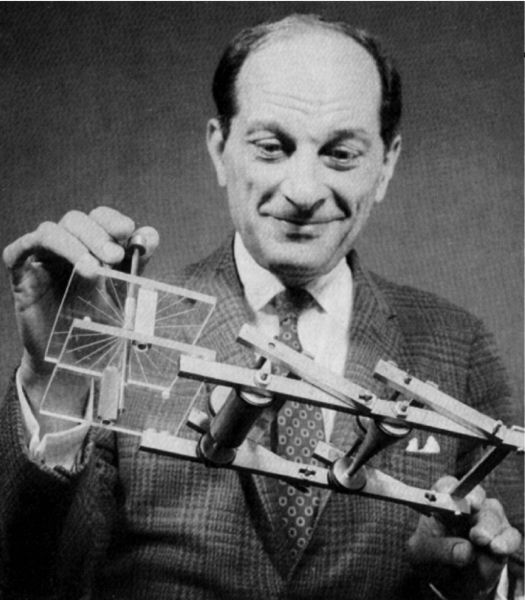
\includegraphics[width=0.25\textwidth]{img/ulam-fermiac.jpg}
\\[2pt] \footnotesize Ulam holding the Fermiac, Enrico Fermi's physical Monte Carlo simulator
  for random neutron diffusion; \hfill
\\[4pt]
{\tiny \mbox{ } \hfill image from G.~C.~Geisler (2000) Los Alamos report LA-UR-2532}
\end{itemize}


\sld{Why Stan?}
%
\begin{itemize}
\item {\slshape\bfseries Goal}: Robust, fully Bayesian inference.
\end{itemize}
%
\vspace*{2pt}
\begin{itemize}
\item {\slshape Problem}: Gibbs and Metropolis too slow (diffusive)
\item {\slshape Solution}: Hamiltonian Monte Carlo (flow)
%
\vspace*{8pt}
\item {\slshape Problem}:  Interpreters slow and unscalable
\item {\slshape Solution}: Compiled to C++
%
\vspace*{8pt}
\item {\slshape Problem}:  Need gradients of log posterior for HMC
\item {\slshape Solution}: Reverse-mode algorithmic differentation
\end{itemize}


\sld{Why Stan? (cont.)}
%
\begin{itemize}
\item {\slshape Problem}:  Existing algo-diff slow, limited, unextensible
\item {\slshape Solution}: Our own algo-diff
%
\vspace*{8pt}
\item {\slshape Problem}:  Algo-diff requires functions templated on
  all args
\item {\slshape Solution}: Our own density library, Eigen linear
 algebra
%
\vspace*{8pt}
\item {\slshape Problem}:  Need unconstrained parameters for HMC
\item {\slshape Solution}: Variable transforms w. Jacobian determinants
%
\end{itemize}


\sld{Why Stan? (cont.)}
%
\begin{itemize}
\item {\slshape Problem}:  Need ease of use of BUGS
\item {\slshape Solution}: Compile a domain-specific language
%
\vspace*{8pt}
\item {\slshape Problem}:  Pure directed graphical language inflexible
\item {\slshape Solution}: Imperative probabilistic programming
  language
\vspace*{8pt}
\item {\slshape Problem}:  Need to tune parameters for HMC
\item {\slshape Solution}: Tune step size and estimate mass matrix
  during warmup;  on-the-fly number of steps (NUTS)
%
\end{itemize}


\sld{Why Stan? (cont.)}
%
\begin{itemize}
%
\vspace*{4pt}
\item {\slshape Problem}:  Efficient up-to-proportion density calcs
\item {\slshape Solution}: Density template metaprogramming
%
\vspace*{4pt}
\item {\slshape Problem}:  Limited error checking, recovery
\item {\slshape Solution}: Static model typing, informative exceptions
%
\vspace*{4pt}
\item {\slshape Problem}:  Poor numerical stability
\item {\slshape Solutions}:
{
Taylor expansions, e.g., {\small \code{log1p()}}
\\[2pt]
compound functions, e.g., {\small \code{log\_sum\_exp()}, \
\code{BernoulliLogit()}}
\\[2pt]
limits at boundaries, e.g., {\small \code{multiply\_log()}}
}
%
\end{itemize}

\sld{Why Stan? (cont.)}
%
\begin{itemize}
\item {\slshape Problem}:  Nobody knows everything
\item {\slshape Solution}: Expand project team with specialists
\vspace*{8pt}
\item {\slshape Problem}:  Expanding code and project team
\item {\slshape Solution}: GitHub: branch, pull
  request, code review
\item {\slshape Solution}: Jenkins: continuous integration
\item {\slshape Solution}: ongoing refactoring and code simplification
%
\end{itemize}

\sld{Why Stan? (cont.)}
%
\begin{itemize}
\item {\slshape Problem}:  Heterogeneous user base
\item {\slshape Solution}: More interfaces (R, Python, MATLAB, Julia)
\item {\slshape Solution}:  domain-specific examples, tutorials
\vspace*{8pt}
\item {\slshape Problem}:  Restrictive licensing limits use
\item {\slshape Solution}: Code and doc open source
(BSD, CC-BY)
\end{itemize}



\mypart{}{MCMC}


\sld{Repeated i.i.d. Trials}
%
\noindent
\begin{minipage}[t]{0.69\textwidth}
\vspace*{-1.9in}
\begin{subitemize}
\item Suppose we repeatedly generate a random outcome from among
several potential outcomes
\item Suppose the outcome chances are the same each time
\begin{subsubitemize}
\item i.e., outcomes are independent and identically distributed (i.i.d.)
\end{subsubitemize}
\item For example, spin a fair spinner (without cheating), such as one from \emph{Family Cricket}.
\end{subitemize}
\end{minipage}
%
\begin{minipage}[t]{0.29\textwidth}
\hfill 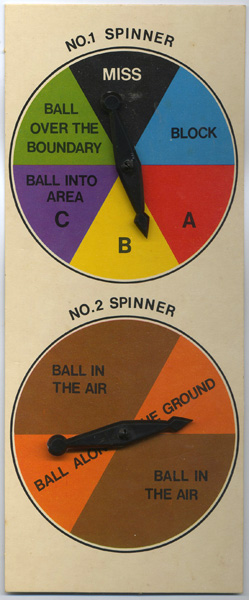
\includegraphics[height=2in]{img/family-cricket-spinner.jpg}
\end{minipage}
\vfill
\hfill {\tiny Image source: \url{http://replaycricket.com/2010/10/29/family-cricket/}}


\sld{Repeated i.i.d. Binary Trials}
%
\begin{itemize}
\item Suppose the outcome is binary and assigned to 0 or 1; e.g.,
\begin{subitemize}
\item 20\% chance of outcome 1: \emph{ball in play}
\item 80\% chance of outcome 0: \emph{ball \emph{not} in play}
\end{subitemize}
\item Consider different numbers of bowls delivered.
\item How will proportion of successes in sample differ?
\end{itemize}


\sld{Simulating i.i.d. Binary Trials}
%
\begin{itemize}
\item R Code: {\small \code{rbinom(10, N, 0.2) / N}}
\begin{subitemize}
\item {\bfseries 10 bowls} \hfill (10\% to 50\% success rate)
\\[4pt] 2 3 5 2 4 1 2 2 1 1
\vspace*{3pt}
%
\item {\bfseries 100 bowls} \hfill (16\% to 26\% success rate)
\\[4pt] 26 18 23 17 21 16 21 15 21 26
\vspace*{3pt}
%
\item {\bfseries 1000 bowls} \hfill (18\% to 22\% success rate)
\\[4pt] 181 212 175 213 216 179 223 198 188 194
\vspace*{3pt}
%
\item {\bfseries 10,000 bowls} \hfill (19.3\% to 20.3\% success rate)
\\[4pt] 2029 1955 1981 1980 2001 2014 1931 1982 1989 2020
\end{subitemize}
\end{itemize}


\sld{Simple Point Estimation}
%
\begin{itemize}
\item Estimate chance of success $\theta$ by proportion of successes:
\[
\theta^{*} = \frac{\text{successes}}{\text{attempts}}
\]
\item Simulation shows accuracy depends on the amount of data.
\item Statistics is about quantifying uncertainty.
\item Bayesian statistics is about using uncertainty in inference.
\end{itemize}


\sld{Confidence via Simulation}
%
\begin{itemize}
\item Estimator uncertainty (\emph{not} Bayesian posterior)
{\small
\begin{Verbatim}
num_sims <- 10000
N <- 100;
theta <- 0.2;
hist(rbinom(num_sims, N, theta) / N,
     main=sprintf("%d simulations",N), xlab="theta*");
\end{Verbatim}
}
\vspace*{-12pt}
\begin{center}
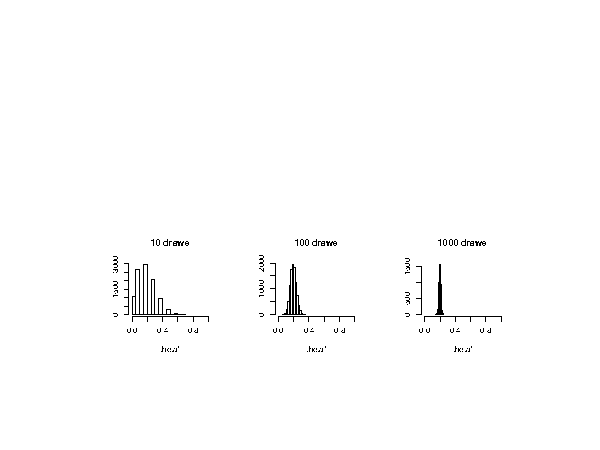
\includegraphics[width=0.8\textwidth]{img/hist-10-100-1000.pdf}
\end{center}
\end{itemize}


\sld{Example Interval Calculation}
%
\begin{itemize}
\item \emph{$P\%$ confidence interval:}  interval in which $P\%$ of the estimates are
expected to fall.
\item Simulation computes intervals to any accuracy.
\item Simulate, sort, and inspect the central empirical interval.
{\small
\begin{Verbatim}
> sims <- rbinom(10000, 1000, 0.2) / 1000
> sorted_sims <- sort(sims)
> sorted_sims[c(250, 9750)]
[1] 0.176 0.225
\end{Verbatim}
}
\item The 95\% confidence interval is thus $(0.176,0.225)$
\item i.e., if true $\theta = 0.2$, then 95\% of the samples of
  size 1000 used will produce estimates in $(0.176,0.225)$
\end{itemize}


\sld{Estimator Bias}
%
\begin{itemize}
\item {\bfseries Bias:} expected difference of estimate from true value
\item Continuing previous example
{\small
\begin{Verbatim}
> sims <- rbinom(10000, 1000, 0.2) / 1000
> mean(sims)
[1] 0.2002536
\end{Verbatim}
}
\item Value of 0.2 is estimate of expectation
\item Shows this estimator is \emph{unbiased}
\end{itemize}


\sld{Simple Point Estimation (cont.)}
%
\begin{itemize}
\item {\bfseries Central Limit Theorem:}  \emph{expected} error in $\theta^*$ goes down as
{\Large
\[
\frac{1}{\sqrt{N}}
\]
}
\item Each decimal place of accuracy requires $100 \times$ more samples.
\item Width of confidence intervals shrinks at the same rate.
\vfill
\item Can also use theory to show this estimator is unbiased.
\end{itemize}


\sld{Pop Quiz! Cancer Clusters}
%
\begin{itemize}
\item Why do lowest and highest cancer clusters look so similar?
\end{itemize}
\vspace*{1pt}
\begin{center}
\hfill
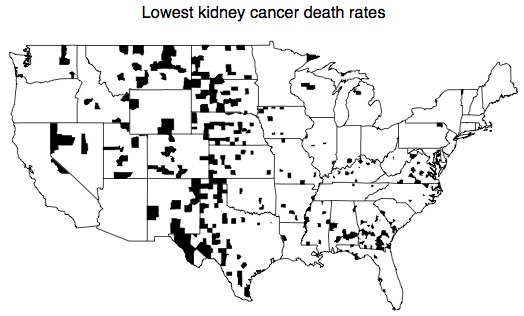
\includegraphics[width=0.45\textwidth]{img/low-cancer.jpg}
\hfill
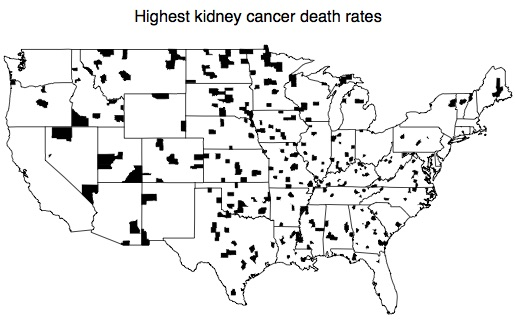
\includegraphics[width=0.45\textwidth]{img/high-cancer.jpg}
\hfill
\end{center}
\vfill
\hfill {\tiny Image from Gelman et al., {\slshape Bayesian Data Analysis, 3rd Edition} (2013)}


\sld{Pop Quiz Answer}
%
\begin{itemize}
\item Hint: mix earlier simulations of repeated i.i.d. trials with 20\% success and sort:
{\footnotesize
\begin{center}
\begin{tabular}{ccccc}
1/10 &  1/10 &  1/10 &  15/100 &  16/100
\\
17/100 &  175/1000 &  179/1000 &  18/100 &  181/1000
\\
188/1000 &  194/1000 &  198/1000 & 2/10 &  2/10
\\
2/10 &  2/10 & 21/100 &  21/100 &  21/100
\\
212/1000 &  213/1000 &   216/1000 &   223/1000 &  23/100
\\
26/100 &  26/100 &  3/10 &  4/10 &  5/10
\end{tabular}
\end{center}
}
\item More variation in observed rates with smaller sample sizes
\vfill
\item \emph{Answer}: High cancer and low cancer counties are small populations
\end{itemize}


\mypart{}{Monte Carlo \\[8pt]\spc Integration}

\sld{Monte Carlo Calculation of $\pi$}

\noindent
\begin{minipage}[t]{0.65\textwidth}
\vspace*{2pt}
\begin{itemize}
\item Computing $\pi = 3.14\ldots$ via simulation is \emph{the} textbook application
of Monte Carlo methods.
\vfill
\item Generate points uniformly at random within the square
\item Calculate proportion within circle ($x^2 + y^2 < 1$) and multiply by square's area (4) to produce the area of the circle.
\item This area is $\pi$ (radius is 1, so area is $\pi r^2 = \pi$)
\end{itemize}
\end{minipage}
%
\begin{minipage}[t]{0.34\textwidth}
\vspace*{12pt}
\hfill 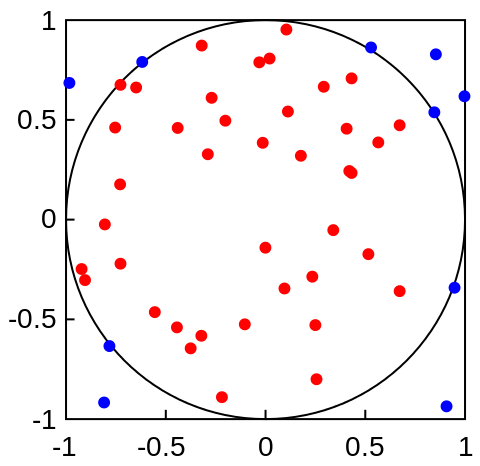
\includegraphics[height=1in]{img/mc-integration-wikipedia.png}
\\
\end{minipage}
\vfill
{ } \hfill {\tiny Plot by Mysid Yoderj courtesy of Wikipedia.}

\sld{Monte Carlo Calculation of $\pi$ {\normalsize (cont.)}}
%
\begin{itemize}
\item R code to calcuate $\pi$ with Monte Carlo simulation:
\\[-8pt]
{\small
\begin{Verbatim}
> x <- runif(1e6,-1,1)
> y <- runif(1e6,-1,1)

> prop_in_circle <- sum(x^2 + y^2 < 1) / 1e6

> 4 * prop_in_circle
[1] 3.144032
\end{Verbatim}
}
\end{itemize}


\sld{Accuracy of Monte Carlo}
%
\begin{itemize}
\item Monte Carlo is \emph{not} that kind of an approximation!
\item It can be made exact to within any $\epsilon$
\item Monte Carlo draws are i.i.d. by definition
\item Central limit theorem: expected error decreases at rate of
{\Large
\[
\frac{1}{\sqrt{N}}
\]
}
\item 3 decimal places of accuracy with
sample size 1e6
\item Need $100 \times$ larger sample for each digit of accuracy
\end{itemize}


\sld{General Monte Carlo Integration}
%
\begin{minipage}[t]{0.69\textwidth}
\vspace*{-0.1in}
\small
\begin{itemize}
\item MC can calculate arbitrary definite integrals,
\[
\int_a^b f(x) \, dx
\]
\item Let $d$ upper bound $f(x)$ in $(a,b)$;  tightness determines
computational efficiency
\item Then generate random points uniformly in the rectangle bounded by $(a,b)$ and $(0,d)$
\item Multiply proportion of draws $(x,y)$ where $y < f(x)$ by area of rectangle, $d \times (b-a)$.
\item Can be generalized to multiple dimensions in obvious way
\end{itemize}
\end{minipage}
\begin{minipage}[t]{0.29\textwidth}
\mbox{ } \\
\mbox{ } \ \ \ \
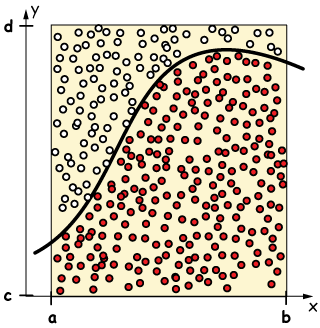
\includegraphics[height=0.9in]{img/monte-carlo-integration.png}
\end{minipage}
\vfill
\hfill
{\tiny Image courtesy of Jeff Cruzan, \url{http://www.drcruzan.com/NumericalIntegration.html}}


\sld{Expectations of Function of R.V.}
%
\begin{itemize}
\item Suppose $f(\theta)$ is a function of random variable vector
  $\theta$
\item Suppose the density of $\theta$ is $p(\theta)$
\begin{subitemize}
\item {\slshape Warning}: $\theta$ overloaded as random and bound variable
\end{subitemize}
\item Then $f(\theta)$ is also random variable, with expectation
  \[
  \mathbb{E}[f(\theta)] = \int_{\Theta} f(\theta) \ p(\theta) \ d\theta.
  \]
\begin{subitemize}
\item
where $\Theta$ is support of $p(\theta)$ (i.e., $\Theta =
\setcomp{\theta \, | \, p(\theta) > 0}$
\end{subitemize}
\end{itemize}


\sld{QoI as Expectations}
%
\begin{itemize}
\item Most Bayesian quantities of interest (QoI) are expectations
  over the posterior $p(\theta \, | \, y)$ of functions $f(\theta)$
\item \myemph{Bayesian parameter estimation}: $\hat{\theta}$
\begin{subitemize}
\item $f(\theta) = \theta$
\item $\hat{\theta} = \mathbb{E}[\theta | y]$ minimizes expected
  square error
\end{subitemize}
\item \myemph{Bayesian parameter (co)variance estimation}:
  $\mathrm{var}[\theta \, | \, y]$
\begin{subitemize}
\item $f(\theta) = (\theta - \hat{\theta})^2$
\end{subitemize}
\item \myemph{Bayesian event probability}:  $\mbox{Pr}[A \, | \, y]$
\begin{subitemize}
  \item $f(\theta) = \mathrm{I}(\theta \in A)$
\end{subitemize}
\end{itemize}


\sld{Expectations via Monte Carlo}
%
\begin{itemize}
\item Generate draws $\theta^{(1)}, \theta^{(2)}, \ldots,
  \theta^{(M)}$ drawn from $p(\theta)$
\item Monte Carlo Estimator \myemph{plugs in average} for expectation:
  \[
  \mathbb{E}[f(\theta)|y] \approx \frac{1}{M} \sum_{m=1}^M f(\theta^{(m)})
  \]
\item Can be made \myemph{as accurate as desired}, because
\[
\mathbb{E}[f(\theta)]
=
\lim_{M \rightarrow \infty} \
\frac{1}{M} \sum_{m=1}^M f(\theta^{(m)})
\]
\vfill
\item {\slshape Reminder}:  By CLT, error goes down as
$1 \, / \, \sqrt{M}$
\end{itemize}


\sld{Monte Carlo for Expectations}
%
\begin{itemize}
\item Most quantities of interest are expectations
\item Suppose $f(\theta)$ is a function of random variable vector $\theta$
  \[
  \mathbb{E}[f(\theta)] = \int_{\Theta} f(\theta) \ p(\theta) \ d\theta.
  \]
where $\Theta$ is support of $p(\theta)$ (i.e., $\Theta =
\setcomp{\theta \, | \, p(\theta) > 0}$)
\item Generate samples $\theta^{(1)}, \theta^{(2)}, \ldots,
  \theta^{(M)}$ drawn from $p(\theta)$
\item Monte Carlo Estimator plugs in average for expectation:
  \[
  \mathbb{E}[f(\theta)|y] \approx \frac{1}{M} \sum_{m=1}^M f(\theta^{(m)})
  \]
\item This technique can be made as accurate as desired, because
\[
\mathbb{E}[f(\theta)]
=
\lim_{M \rightarrow \infty}
\frac{1}{M} \sum_{m=1}^M f(\theta^{(m)})
\]
\end{itemize}


\mypart{}{Markov Chain \\[8pt]\spc{}Monte Carlo}


\sld{Markov Chain Monte Carlo}
%
\begin{itemize}
\item Standard Monte Carlo draws i.i.d. samples
\[
\theta^{(1)}, \ldots, \theta^{(M)}
\]
according to a probability function $p(\theta)$
\item Drawing i.i.d. samples typically impossible for
  complex densities like Bayesian posteriors $p(\theta|y)$
\item Instead, use Markov chain Monte Carlo (MCMC) to
  draw $\theta^{(1)}, \ldots, \theta^{(M)}$ from a Markov chain
  with appropriate stationary distribution $p(\theta | y)$.
\end{itemize}


\sld{Markov Chains}
%
\begin{itemize}
\item A Markov Chain is a sequence of random variables
\[
\theta^{(1)},
  \theta^{(2)}, \ldots, \theta^{(M)}
\]
such that $\theta^{(m)}$ only depends on $\theta^{(m-1)}$, i.e.,
\[
p(\theta^{(m)} | y, \theta^{(1)}, \ldots, \theta^{(m-1)})
\ = \
p(\theta^{(m)} | y, \theta^{(m-1)})
\]
\item Drawing $\theta^{(1)}, \ldots, \theta^{(M)}$ from a Markov chain
  according to \\ $p(\theta^{(m)} \, | \, \theta^{(m-1)}, y)$ is more tractable
\item Require marginal of each draw, $p(\theta^{(m)}|y)$,
  to be equal to true posterior
\item Otherwise, apply just like ordinary (non-Markov chain) Monte Carlo methods
\end{itemize}


\sld{Applying MCMC}
%
\begin{itemize}
\item Plug in just like ordinary (non-Markov chain) Monte Carlo
\item Adjust standard errors for dependence in Markov chain
\end{itemize}


\sld{MCMC for Posterior Mean}
%
\begin{itemize}
\item Standard Bayesian estimator is posterior mean
\[
\hat{\theta}  \ =  \ \int_{\Theta} \theta \, p(\theta|y) \, d\theta
\]
\begin{subitemize}
\item Posterior mean minimizes expected square error
\end{subitemize}
\item Estimate is a conditional expectation
\[
\hat{\theta} = \mathbb{E}[\theta|y]
\]
\item Compute by averaging
\[
\hat{\theta} \ \approx \ \frac{1}{M} \sum_{m=1}^M \theta
\]
\end{itemize}


\sld{MCMC for Posterior Variance}
%
\begin{itemize}
\item Posterior variance works the same way, given previous result
\[
\expectation{(\theta - \expectation{\theta})^2}
\approx \frac{1}{M} \sum_{m=1}^M (\theta^{(m)} - \hat{\theta})^2
\]
\end{itemize}


\sld{MCMC for Posterior Median}
%
\begin{itemize}
\item Alternative Bayesian estimator is posterior median
\begin{subitemize}
\item Posterior median minimizes expected absolute error
\end{subitemize}
\item Calculate as middle draw of $\theta^{(1)}, \ldots,
  \theta^{(M)}$
\begin{subitemize}
\item just sort and take halfway value
\item e.g., Stan shows 50\% point (or other quantiles)
\end{subitemize}
\end{itemize}


\sld{MCMC for Event Probability}
%
\begin{itemize}
\item Event probabilities are also expectations, e.g.,
\[
\Prob{\theta_1 > \theta_2}
\ = \ \expectation{\indicator{\theta_1 > \theta_2}}
\ = \ \int_{\Theta} \indicator{\theta_1 > \theta_2} \, p(\theta|y) d\theta.
\]
\item Estimation via MCMC just another plug-in:
\[
\Prob{\theta_1 > \theta_2} \approx
\frac{1}{M} \sum_{m=1}^M \indicator{\theta_1^{(m)} > \theta_2^{(m)}}
\]
\item Again, can be made as accurate as necessary
\end{itemize}


\sld{MCMC for Quantiles (incl.\ median)}
%
\begin{itemize}
\item These are not expectations, but still plug in
\item Alternative Bayesian estimator is posterior median
\begin{subitemize}
\item Posterior median minimizes expected absolute error
\end{subitemize}
\item Estimate as median draw of $\theta^{(1)}, \ldots,
  \theta^{(M)}$
\begin{subitemize}
\item just sort and take halfway value
\item e.g., Stan shows 50\% point (or other quantiles)
\end{subitemize}
\item Other quantiles including interval bounds similar
\begin{subitemize}
\item estimate with quantile of draws
\item estimation error goes up in tail (based on fewer draws)
\end{subitemize}
\end{itemize}


\mypart{}{MCMC Algorithms}


\sld{Random-Walk Metropolis}
%
\begin{itemize}
\item Draw random initial parameter vector $\theta^{(1)}$ (in
  support)
\item For $m \in \range{2}{M}$
\hspace*{-8pt}
\begin{subitemize}
\item Sample proposal from a (symmetric) jumping distribution, e.g.,
\[
\theta^*
\ \sim \
\distro{MultiNormal}(\theta^{(m-1)}, \ \sigma \mbox{\bfseries I})
\]
where {\bfseries I} is the identity matrix
\item
\vspace*{4pt}
Draw $u^{(m)} \sim \distro{Uniform}(0,1)$ and set
\[
\theta^{(m)}
\ = \
\begin{cases}
\theta^{*}
  & \text{if } u^{(m)} < {\displaystyle \frac{p(\theta^{*}|y)}{p(\theta^{(m)}|y)}}
\\[8pt]
\theta^{(m-1)}
  & \text{otherwise}
\end{cases}
\]
\end{subitemize}
\end{itemize}


\sld{Metropolis and Normalization}
%
\begin{itemize}
\item Metropolis only uses posterior in a ratio:
\[
\frac{p(\theta^{*} \, | \, y)}
     {p(\theta^{(m)} \, | \, y)}
\]
\item This allows the use of unnormalized densities
\item Recall Bayes's rule:
\[
p(\theta | y) \propto p(y|\theta) \, p(\theta)
\]
\item Thus we only need to evaluate sampling (likelihood) and prior
\item It also sidesteps computing the normalizing term
\[
\int_{\Theta} p(y|\theta) \, p(\theta) d\theta
\]
\end{itemize}


\sld{Metropolis-Hastings}
%
\begin{itemize}
\item Generalizes Metropolis to asymmetric proposals
\item Acceptance ratio is
\[
\frac{J(\theta^{(m)}|\theta^{*}) \ \times \ p(\theta^{*}|y)}
     {J(\theta^{*}|\theta^{(m-1)}) \ \times \ p(\theta^{(m)}|y)}
\]
where $J$ is the (potentially asymmetric) proposal density
\item i.e.,
{\small
\[
\frac{\mbox{probabilty of being at } \theta^*
      \mbox{ and jumping to } \theta^{(m-1)}}
     {\mbox{probability of being at } \theta^{(m-1)}
      \mbox{ and jumping to } \theta^{*}}
\]
}
\vspace*{3pt}
\item General form ensures equilibrium
  by maintaining \emph{detailed balance}
\item Like Metropolis, only requires ratios
\item Many algorithms involve a Metropolis-Hastings ``correction''
\end{itemize}


\sld{Detailed Balance \& Reversibility}
%
\begin{itemize}
\item Definition is measure theoretic, but applies to densities
\begin{subitemize}
\item just like Bayes's rule
\end{subitemize}
\item Assume Markov chain has stationary density $p(a)$
\item Suppose $\pi(a | b)$ is density of
  transitioning from $b$ to $a$
\begin{subitemize}
\item use of $\pi$ to indicates different measure on $\Theta$ than $p$
\end{subitemize}
\item Detailed balance is a reversibility equilibrium condition
\[
p(a) \,\pi(b | a)
\ = \
p(b) \, \pi(a | b)
\]
\end{itemize}


\sld{Optimal Proposal Scale?}
%
\begin{itemize}
\item Proposal scale $\sigma$ is a free; too low or high is inefficient
\begin{center}
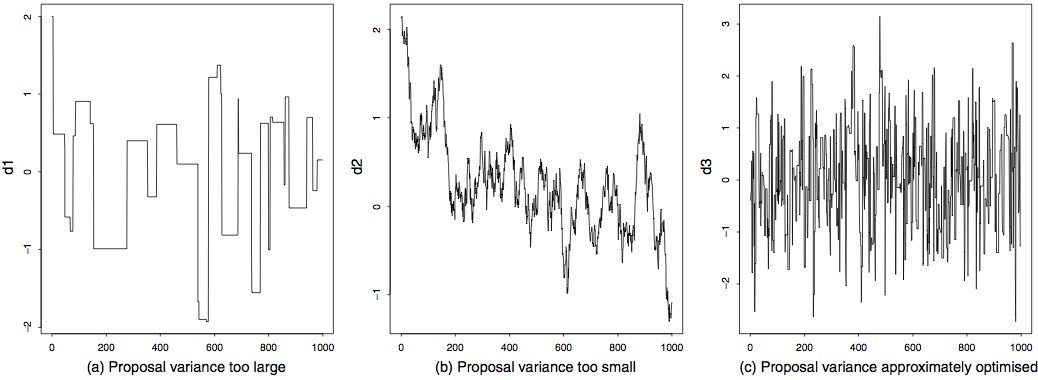
\includegraphics[width=0.9\textwidth]{img/roberts-rosenthal-traceplots.jpg}
\end{center}
\item \emph{Traceplots} show parameter value on $y$ axis, iterations on $x$
\item Empirical tuning problem; theoretical optima exist for some
  cases
\end{itemize}
\vfill\hfill
{\tiny Roberts and Rosenthal (2001) Optimal Scaling for Various
  Metropolis-Hastings Algorithms. {\slshape Statistical Science}.}


\sld{Convergence and Stationarity}
%
\begin{itemize}
\item Imagine releasing a hive of bees in a sealed house
\begin{subitemize}
\item they disperse, but eventually reach equilibrium where the same
  number of bees leave a room as enter it (on average)
\end{subitemize}
\item May take many iterations for Markov chain to reach equilibrium
\vspace*{3pt}
\begin{center}
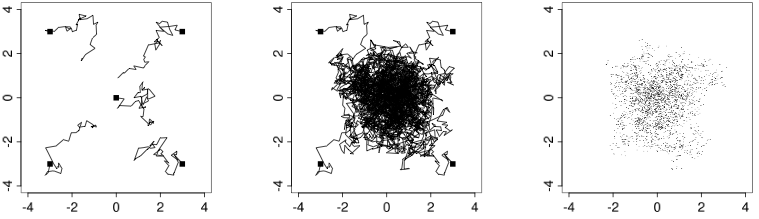
\includegraphics[width=0.8\textwidth]{img/bda-diffuse-converge.png}
\end{center}
\item Four chains with different starting points
\item \emph{Left}) 50 iterations;  \emph{Center}) 1000 iterations;  \emph{Right}) Draws from second half of each chain
\end{itemize}


\sld{Potential Scale Reduction ($\hat{R}$)}
%
\begin{itemize}
\item Gelman \& Rubin recommend $M$ chains of $N$ draws with
  \myemph{diffuse initializations}
\item Measure that each chain has same posterior mean and variance
\item If not, may be stuck in multiple modes or just not converged yet
\item Define statistic $\hat{R}$ of chains such that \myemph{at convergence},
$\hat{R} \rightarrow 1$
\begin{subitemize}
\item $\hat{R} >\!> 1$ implies non-convergence
\item $\hat{R} \approx 1$ \myemph{does not guarantee convergence}
\item Only measures marginals
\end{subitemize}
\end{itemize}


\sld{Split $\hat{R}$}
\begin{itemize}
\item Vanilla $\hat{R}$ may not diagnose non-stationarity
\begin{subitemize}
\item e.g., a sequence of chains with an increasing parameter
\end{subitemize}
\item \myemph{Split $\hat{R}$}: \ Stan splits each chain into first and
  second half
\begin{subitemize}
\item start with $M$ Markov chains of $N$ draws each
\item split each in half to creates $2M$ chains of $N/2$ draws
\item then apply $\hat{R}$ to the $2M$ chains
\end{subitemize}
\end{itemize}


\sld{Calculating $\hat{R}$ Statistic}
%
\begin{itemize}
\item \myemph{Between-sample variance} estimate
\[\textstyle
B
= \frac{N}{M-1} \, \sum_{m=1}^M (\bar{\theta}^{(\bullet)}_{m} - \bar{\theta}^{(\bullet)}_{\bullet})^2,
\]
%
where
%
\[\textstyle
\bar{\theta}_m^{(\bullet)}
= \frac{1}{N} \sum_{n = 1}^N \theta_m^{(n)}
\ \ \ \ \
\mbox{and}
\ \ \ \ \
\bar{\theta}^{(\bullet)}_{\bullet}
= \frac{1}{M} \, \sum_{m=1}^M \bar{\theta}_m^{(\bullet)}.
\]
\vspace*{6pt}
\item \myemph{Within-sample variance} estimate:
\[\textstyle
W
= \frac{1}{M} \, \sum_{m=1}^M s_m^2,
\]
where
\[\textstyle
s_m^2 = \frac{1}{N-1} \, \sum_{n=1}^N (\theta^{(n)}_m - \bar{\theta}^{(\bullet)}_m)^2.
\]
\end{itemize}


\sld{Calculating $\hat{R}$ Statistic (cont.)}
%
\begin{itemize}
\item \myemph{Variance} estimate:
\[\textstyle
\widehat{\mbox{var}}^{+}\!(\theta|y)
= \frac{N-1}{N}\, W \, + \, \frac{1}{N} \, B.
\]
%
\vspace*{6pt}
\item \myemph{Potential scale reduction} statistic (``R hat'')
\[\textstyle
\hat{R}
\, = \,
\sqrt{\frac{\widehat{\mbox{var}}^{+}\!(\theta|y)}{W}}.
\]
\end{itemize}


\sld{Correlations in Posterior Draws}
%
\begin{itemize}
\item Markov chains typically display autocorrelation in the series of
  draws $\theta^{(1)}, \ldots, \theta^{(m)}$
\item Without i.i.d. draws, central limit theorem \emph{does not apply}
\item Effective sample size $N_{\mbox{\footnotesize eff}}$ divides out
  autocorrelation
\item $N_{\mbox{\footnotesize eff}}$ must be estimated from sample
\begin{subitemize}
\item Fast Fourier transform to efficiently computes correlations at all lags
\end{subitemize}
\vspace*{-6pt}
\item Estimation accuracy proportional to
{\Large
\[
\frac{1}{\sqrt{N_{\mbox{\normalsize eff}}}}
\]
}
\item Compare previous plots; good choice of $\sigma$ leads to high
$N_{\mbox{\footnotesize eff}}$
\end{itemize}


\sld{Effective Sample Size (ESS)}
%
\begin{itemize}
\item Autocorrelation at lag $t$ is correlation between subsequences
\begin{subitemize}
\item $(\theta^{(1)},\ldots, \theta^{(N-t)})$ and $(\theta^{(1 + t)}, \ldots, \theta^{(N)})$
\end{subitemize}
\item  Suppose chain has density $p(\theta)$ with
\begin{subitemize}
\item $\mathbb{E}[\theta] = \mu$ \ \ and \ \ $\mbox{\rm Var}[\theta] = \sigma^2$
\end{subitemize}
\item Autocorrelation $\rho_t$ at lag $t \geq 0$:
\[
\rho_t  =  \frac{1}{\sigma^2} \, \int_{\Theta} (\theta^{(n)} - \mu)
       (\theta^{(n+t)} - \mu) \, p(\theta) \, d\theta
\]
\item Because $p(\theta^{(n)}) = p(\theta^{(n+t)}) = p(\theta)$ at convergence,
\[
\rho_t = \frac{1}{\sigma^2} \, \int_{\Theta} \theta^{(n)} \, \theta^{(n+t)} \, p(\theta) \, d\theta
\]
\end{itemize}


\sld{Estimating Autocorrelations}
%
\begin{itemize}
\item Effective sample size is defined by
\[\textstyle
N_{\mbox{\scriptsize eff}}
\ = \
\frac{N}{\sum_{t = -\infty}^{\infty} \rho_t}
\ = \
\frac{N}{1 + 2 \sum_{t = 1}^{\infty} \rho_t}
\]
\item Estimate in terms of variograms at lag $t$,
\[\textstyle
V_t =
\frac{1}{M}
\,
\sum_{m=1}^M
\
\left(
\frac{1}{N_m - t}
\sum_{n=t+1}^{N_m}
\left(
\theta_m^{(n)} - \theta_m^{(n-t)}
\right)^2
\right)
\]
\item Estimate autocorrelation at lag $t$ using cross-chain variance
  as
\[
\hat{\rho}_t
= 1 - \frac{\displaystyle V_t}{
            \displaystyle 2 \, \widehat{\mbox{var}}^{+}}
\]
\item If not converged, $\widehat{\mbox{var}}^{+}$ overestimates variance
\item Efficiently calculate using fast Fourier transform (w.\ padding)
\end{itemize}


\sld{Estimating $N_{\normalsize eff}$}
%
\begin{itemize}
\item Let $T'$ be first lag s.t.\ $\rho_{T' + 1} < 0$,
\item Estimate autocorrelation by
\[
\hat{N}_{\mbox{\scriptsize eff}}
=
\frac{MN}
     {1 + \sum_{t=1}^{T'} \hat{\rho}_t}.
\]
\item NUTS avoids negative autocorrelations, so first negative
  autocorrelation estimate is reasonable
\vfill
\item See {\footnotesize Charles Geyer (2013) Introduction to MCMC. In
    {\slshape Handbook of MCMC}.
 (free online at \url{http://www.mcmchandbook.net/index.html})}
\end{itemize}


\sld{Gibbs Sampling}
%
\begin{itemize}
\item Draw random initial parameter vector $\theta^{(1)}$ (in
  support)
\item For $m \in \range{2}{M}$
\begin{subitemize}
\item For $n \in \range{1}{N}$:
\begin{itemize}
\item draw
$\theta^{(m)}_n$ according to conditional \\[8pt]
$p(\theta_n|\theta_1^{(m)},\ldots,\theta_{n-1}^{(m)}, \, \theta_{n+1}^{(m-1)},
\ldots,\theta_N^{(m-1)},  y)$.
\end{itemize}
\end{subitemize}
\item e.g, with $\theta = (\theta_1,\theta_2,\theta_3)$:
\begin{subitemize}
\item draw \ $\theta_1^{(m)}$  \ according to \ $p(\theta_1 | \theta_2^{(m-1)},
  \theta_3^{(m-1)}, y)$
\item draw \ $\theta_2^{(m)}$ \ according to \ $p(\theta_2 | \theta_1^{(m)},
  \theta_3^{(m-1)}, y)$
\item draw \ $\theta_3^{(m)}$ \ according to \ $p(\theta_3 | \theta_1^{(m)},
  \theta_2^{(m)}, y)$
\end{subitemize}
\end{itemize}


\sld{Generalized Gibbs}
%
\begin{itemize}
\item ``Proper'' Gibbs requires the conditional Monte Carlo draws
\begin{subitemize}
\item typically works only for conjugate priors
\end{subitemize}
\item In general case, may need to use less efficient conditional
  draws
\begin{subitemize}
\item Slice sampling is a popular general technique that works for
  discrete or continuous $\theta_n$
\item Adaptive rejection sampling is another alternative
\item Very difficult in more than one or two dimensions
\end{subitemize}
\end{itemize}


\sld{Sampling Efficiency}
%
\begin{itemize}
\item We care only about $N_{\mbox{\footnotesize eff}}$ per second
\item Decompose into
{\small
\begin{enumerate}
\item Iterations per second
\item Effective samples per iteration
\end{enumerate}
}
\item Gibbs and Metropolis have high iterations per second (especially
  Metropolis)
\item But they have low effective samples per iteration (especially
  Metropolis)
\item Both are particular weak when there is high correlation among
  the parameters in the posterior
\end{itemize}


\sld{Hamiltonian Monte Carlo \& NUTS}
%
\begin{itemize}
\item Slower iterations per second than Gibbs or Metropolis
\item Much higher number of effective samples per iteration for
complex posteriors (i.e., high curvature and correlation)
\item Overall, much higher $N_{\mbox{\footnote eff}}$ per second
\vfill
\item Details in the next talk \ldots
\item Along with details of how Stan implements HMC and NUTS
\end{itemize}



\mypart{}{Bayesian Inference}


\sld{Bayesian Data Analysis}
%
\begin{itemize}
\item ``By {Bayesian data analysis}, we mean {practical methods}
  for making {inferences} from {data} using {probability models}
  for quantities we {observe} and about which we {wish to learn}.''
  %
\item ``The essential characteristic of Bayesian methods is
  their \myemph{explict use of probability for quantifying uncertainty}
  in inferences based on statistical analysis.''
\end{itemize}
%
\vfill\hfill{\footnotesize Gelman et al., {\slshape Bayesian Data Analysis},
  3rd edition, 2013}


\sld{Bayesian Methodology}
%
\begin{itemize}
\item Set up \myemph{full probability model}
  \vspace*{-4pt}
  \begin{itemize}
  \item for \myemph{all} observable \& unobservable quantities
  \item consistent w. problem knowledge \& data collection
  \end{itemize}
  %
\item \myemph{Condition} on observed data (where Stan comes in!)
  \vspace*{-4pt}
  \begin{itemize}
  \item to caclulate posterior probability of unobserved quantities
    (e.g., parameters, predictions, missing data)
  \end{itemize}
  %
\item \myemph{Evaluate}
  \vspace*{-4pt}
  \begin{itemize}
  \item model fit and implications of posterior
  \end{itemize}
\vfill
\item \myemph{Repeat} as necessary
\end{itemize}
\vfill\hfill {\footnotesize {\slshape Ibid.}}


\sld{Where do Models Come from?}
%
\begin{itemize}
\item Sometimes model comes first, based on substantive
  considerations
\begin{subitemize}
\item toxicology, economics, ecology, physics, \ldots
\end{subitemize}
\item Sometimes model chosen based on data collection
\begin{subitemize}
\item  traditional statistics of surveys and experiments
\end{subitemize}
\item Other times the data comes first
\begin{subitemize}
\item observational studies, meta-analysis, \ldots
\end{subitemize}
\hfill
\item Usually its a mix
\end{itemize}


\sld{Model Checking}
%
\begin{itemize}
\item Do the inferences make sense?
\begin{subitemize}
\item are parameter values consistent with model's prior?
\item does simulating from parameter values produce reasoable fake
  data?
\item are marginal predictions consistent with the data?
\end{subitemize}
\item Do predictions and event probabilities for new data make sense?
\vfill
\item {\slshape \myemph{Not}}: Is the model true?
\item {\slshape \myemph{Not}}: What is Pr[model is true]?
\item {\slshape \myemph{Not}}: Can we ``reject'' the model?
\end{itemize}


\sld{Model Improvement}
%
\begin{itemize}
\item Expanding the model
\begin{subitemize}
\item hierarchical and multilevel structure \ldots
\item more flexible distributions (overdispersion, covariance)
\item more structure (geospatial, time series)
\item more modeling of measurement methods and errors
\item \ldots
\end{subitemize}
\item Including more data
\begin{subitemize}
\item breadth (more predictors or kinds of observations)
\item depth (more observations)
\end{subitemize}
\end{itemize}


\sld{Properties of Bayesian Inference}
%
\begin{itemize}
\item Explores full range of parameters consistent with prior info and
  data$^*$
\begin{subitemize}
\item $^*$ if such agreement is possible
\item Stan automates this procedure with diagnostics
\end{subitemize}
\item Inferences can be plugged in directly for
\begin{subitemize}
\item parameter estimates minimizing expected error
\item predictions for future outcomes with uncertainty
\item event probability updates conditioned on data
\item risk assesment / decision analysis conditioned on uncertainty
\end{subitemize}
\end{itemize}


\sld{Notation for Basic Quantities}
%
\begin{itemize}
\item \myemph{Basic Quantities}
\begin{subitemize}
\item $y$: \ observed data
\item $\theta$: \ parameters (and other unobserved quantities)
\item $x$: \ constants, predictors for conditional (aka ``discriminative'') models
\end{subitemize}
\item \myemph{Basic Predictive Quantities}
\begin{subitemize}
\item $\tilde{y}$: unknown, potentially observable quantities
\item $\tilde{x}$: \ constants, predictors for unknown quantities
\end{subitemize}
\end{itemize}


\sld{Naming Conventions}
%
\begin{itemize}
\item \myemph{Joint}: \ $p(y,\theta)$
\item \myemph{Sampling / Likelihood}: \ $p(y|\theta)$
\begin{subitemize}
\item Sampling is function of $y$ with $\theta$ fixed (prob function)
\item Likelihood is function of $\theta$ with $y$ fixed (\emph{not} prob function)
\end{subitemize}
\item \myemph{Prior}: \ $p(\theta)$
\item \myemph{Posterior}: \ $p(\theta|y)$
\item \myemph{Data Marginal (Evidence)}: \ $p(y)$
\item \myemph{Posterior Predictive}: \ $p(\tilde{y}|y)$
\end{itemize}


\sld{Bayes's Rule for Posterior}
%
\vspace*{-4pt}
\begin{eqnarray*}
    p(\theta|y)
    & = & \frac{p(y,\theta)}{p(y)}
          \hspace*{64pt} \text{\small [def of conditional]}
    \\[6pt]
    & = & \frac{p(y|\theta) \, p(\theta)}{p(y)}
          \hspace*{44pt} \text{\small [chain rule]}
    \\[6pt]
    & = & \frac{p(y|\theta) \, p(\theta)}{\int_{\Theta} p(y,\theta') \ d\theta'}
          \hspace*{40pt} \text{\small [law of total prob]}
    \\[6pt]
    & = & \frac{p(y|\theta) \, p(\theta)}{\int_{\Theta} p(y|\theta') \,
      p(\theta') \ d\theta'}
          \hspace*{20pt} \text{\small [chain rule]}
\end{eqnarray*}
\vfill
\begin{itemize}
\item \emph{Inversion:} Final result depends only on
  sampling distribution (likelihood) $p(y|\theta)$ and prior
  $p(\theta)$
\end{itemize}


\sld{Bayes's Rule up to Proportion}
%
\begin{itemize}
\item If data $y$ is fixed, then
\begin{eqnarray*}
p(\theta|y)
& = & \frac{p(y|\theta) \, p(\theta)}{p(y)}
\\[6pt]
& \propto & p(y|\theta) \, p(\theta)
\\[6pt]
& = & p(y,\theta)
\end{eqnarray*}
\item Posterior proportional to likelihood times prior
\item Equivalently, posterior proportional to joint
\vfill
\item The nasty integral for data marginal $p(y)$ goes away
\end{itemize}


\sld{Posterior Predictive Distribution}
%
\begin{itemize}
\item Predict new data $\tilde{y}$ based on observed data $y$
\item Marginalize parameters $\theta$ out of posterior and likelihood
\begin{eqnarray*}
p(\tilde{y} \mid y)
& = & \mathbb{E}[p(\tilde{y} | \theta) \mid Y = y]
\\[6pt]
& = &
\int p(\tilde{y} | \theta) \, p(\theta | y) \, d\theta.
\end{eqnarray*}
\item Weights predictions $p(\tilde{y}|\theta)$,
by posterior $p(\theta|y)$
\item Integral notation shorthand for sums and/or integrals
\end{itemize}


\sld{Posterior Event Probabilities}
%
\begin{itemize}
\item Recall that an event $A$ is a collection of outcomes
\item So $A$ may be defined by an indicator $f$ on parameters
\[
f(\theta)
=
\begin{cases}
1 & \text{if } \theta \in A
\\
0 & \text{if } \theta \not\in A
\end{cases}
\]
\begin{subitemize}
\item $f(\theta) = \mathrm{I}(\theta_1 > \theta_2)$
\ \ for \ \ $\Prob{\theta_1 > \theta_2 \, | \, y}$,
\item $f(\theta) = \mathrm{I}(\theta \in (0.50, 0.52)$ for $\mathrm{Pr}\left[ \theta \in (0.50, 0.52) \,|\, y \right]$
\end{subitemize}
\item Defined by posterior expectation of indicator $f(\theta)$
\[
\mathrm{Pr}[A \,|\, y]
\ = \
\mathbb{E}\left[ f(\theta) \, | \, y \right]
\ = \
\int_{\Theta} f(\theta) \, p(\theta|y) \, d\theta.
\]
\end{itemize}


\sld{Event Probabilities}
%
\begin{itemize}
\item An \myemph{event} $A$ is a collection of outcomes
\item So $A$ may be defined by an indicator $f$ on parameters $\theta$,
\[
f(\theta)
=
\begin{cases}
1 & \text{if } \theta \in A
\\
0 & \text{if } \theta \not\in A
\end{cases}
\]
\item e.g., $f(\theta) = \theta_1 > \theta_2$
\ \ for \ \ $\Prob{\theta_1 > \theta_2 \, | \, y}$
\item Bayesian event probabilities calculate posterior mass
\[
\Prob{A} = \int_{\Theta} f(\theta) \, p(\theta|y) \, d\theta.
\]
\item Not frequentist, because involves parameter probabilities
\end{itemize}


\sld{Event Probabilities}
%
\begin{itemize}
\item Events are fundamental probability bearing units which
\begin{subitemize}
\item are defined by sets of outcomes
\item which occur or not with some probability
\end{subitemize}
\item Events typically defined as conditions on random variables, e.g.,
\begin{subitemize}
\item $\theta_b > \theta_g$ for more boy births than girl births
\item $z_k = 1$ for team A beating team B in game $k$
\end{subitemize}
\end{itemize}


\sld{Event Probabilities in Stan}
%
\begin{itemize}
\item MCMC estimates
\[
\mathrm{Pr}[A \, | \, y]
\approx
\sum_{m=1}^M f(\theta^{(m)})
\]
with posterior draws $\theta^{(1)}, \ldots, \theta^{(M)}$.
\vfill
\item In Stan, only need to define a variable in generated quantities
  block for the indicator
\begin{stancode}
generated quantities {
  int<lower=0, upper=1> theta_gt_half = (theta > 0.5);
}
\end{stancode}
\end{itemize}


\sld{Event Probabilities, cont.}
%
\begin{itemize}
\item $\theta = (\theta_1, \ldots, \theta_N)$ is a sequence of
  random variables
\item $c$ is a condition on $\theta$,
  so that $c(\theta_1, \ldots, \theta_N) \in \{ 0, 1 \}$
\item Suppose $Y = y$ is some observed data
\item The probability that the event holds conditioned on the data is
  given by
%
\begin{eqnarray*}
\Prob{c(\theta_1, \ldots, \theta_N) | Y = y}
& = & \mathbb{E}[c(\theta_1,\ldots, \theta_N) \mid Y]
\\[6pt]
& = & \int c(\theta) \, p(\theta|y) \, \mathrm{d}\theta
\end{eqnarray*}
%
\item Not frequentist, because involves parameter probabilities
\end{itemize}


\mypart{}{Conjugate Priors}


\sld{Conjugate Priors}
%
\begin{itemize}
\item Family $\mathcal{F}$ is a conjugate prior for family
  $\mathcal{G}$ if
\begin{subitemize}
\item prior in $\mathcal{F}$ and
\item likelihood in $\mathcal{G}$,
\item entails posterior in $\mathcal{F}$
\end{subitemize}
\item Before MCMC techniques became practical, Bayesian analysis
  mostly involved conjugate priors
\item Still widely used because analytic solutions are more efficient
  than MCMC
\end{itemize}

\sld{Beta is Conjugate to Binomial}
%
\vspace*{-2pt}
\begin{itemize}
\item Prior: \ \ \ \ \ \ \ \ \ \ \ $p(\theta|\alpha,\beta) =
  \distro{Beta}(\theta|\alpha,\beta)$
\item Likelihood: \ \ $p(y|N,\theta) = \distro{Binomial}(y|N,\theta)$
\item Posterior:
{\small
\begin{eqnarray*}
p(\theta|y,N,\alpha,\beta)
& \propto & p(\theta|\alpha,\beta) \, p(y|N,\theta)
\\[6pt]
& = & \distro{Beta}(\theta|\alpha,\beta)
      \, \distro{Binomial}(y|N,\theta)
\\
& = & \frac{1}{\Betafun(\alpha,\beta)}
      \theta^{\alpha - 1} \,
      (1 - \theta)^{\beta-1}
      \ \
      \binom{N}{y} \theta^{y} (1 - \theta)^{N-y}
\\[6pt]
& \propto &
      \theta^{y + \alpha - 1} \,
      (1 - \theta)^{N - y + \beta - 1}
\\[6pt]
& \propto & \distro{Beta}(\theta|\alpha + y, \ \beta + (N - y))
\end{eqnarray*}
}
\end{itemize}


\sld{Chaining Updates}
%
\vspace*{-4pt}
\begin{itemize}
\item Start with prior $\distro{Beta}(\theta|\alpha,\beta)$
\item Receive binomial data in $K$ statges $(y_1, N_1), \ldots, (y_K, N_K)$
\item After $(y_1,N_1)$, posterior is
  $\distro{Beta}(\theta|\alpha + y_1, \ \beta + N_1 - y_1)$
\item Use as prior for $(y_2,N_2)$, with posterior \\[3pt]
  $\distro{Beta}(\theta|\alpha + y_1 + y_2, \ \ \beta + (N_1 -
  y_1) + (N_2 - y_2))$
\item Lather, rinse, repeat, until final posterior
\[
\distro{Beta}(\theta|\alpha + y_1 + \cdots + y_K, \ \ \beta + (N_1 +
\cdots + N_K) - (y_1 + \cdots + y_K))
\]
\item Same result as if we'd updated with combined data \\[3pt]
$\distro{Beta}(y_1 + \cdots + y_K, \ \ N_1 + \cdots + N_K)$
\end{itemize}


\mypart{}{Repeated Binary Trials}


\sld{Repeated Binary Trial Model}
%
\begin{itemize}
%
\vspace*{-4pt}
\item \myemph{Data}
\begin{subitemize}
  \item $N \in \setcomp{0, 1, \ldots}$: number of trials (constant)
  \item $y_n \in \setcomp{0, 1}$: trial $n$ success (known, modeled data)
\end{subitemize}
%
\vspace*{-6pt}
\item \myemph{Parameter}
\begin{subitemize}
\item $\theta \in [0, 1]$ : chance of success (unknown)
\end{subitemize}
%
\vspace*{-6pt}
\item \myemph{Prior}
\begin{subitemize}
\item $p(\theta)
\ = \
\distro{Uniform}(\theta \,|\, 0, 1) = 1$
\end{subitemize}
%
\vspace*{-6pt}
\item \myemph{Likelihood}
\begin{subitemize}
\item $p(y \,|\, \theta)
\ = \ \prod_{n=1}^N \distro{Bernoulli}(y_n \,|\, \theta)
\ = \ \prod_{n=1}^N \theta^{y_n} \, (1 - \theta)^{1 - y_n}$
\end{subitemize}
%
\vspace*{-6pt}
\item \myemph{Posterior}
\begin{subitemize}
\item
$p(\theta \, | \, y)
\propto
p(\theta) \, p(y \, | \, \theta)$
\end{subitemize}
\end{itemize}



\sld{Stan Program}
%
\begin{stancode}
data {
  int<lower=0> N;                 // number of trials
  int<lower=0, upper=1> y[N];     // success on trial n
}
parameters {
  real<lower=0, upper=1> theta;   // chance of success
}
model {
  theta ~ uniform(0, 1);          // prior
  y ~ bernoulli(theta);           // likelihood
}
\end{stancode}


\sld{A Stan Program...}
%
\begin{itemize}
\item defines log (posterior) density up to constant, so...
\item equivalent to define log density directly:
\begin{stancode}
model {
  target += 0;
  for (n in 1:N)
    target += log(y[n] ? theta : (1 - theta));
}
\end{stancode}
\item equivalent to drop constant prior and vectorize
  likelihood:
\begin{stancode}
model {
  y ~ bernoulli(theta);
}
\end{stancode}
\end{itemize}


\sld{R: Simulate Data}
%
\begin{itemize}
\item Generate data
\begin{codein}
> theta <- 0.30;
> N <- 20;
> y <- rbinom(N, 1, 0.3);

> y
\end{codein}
\begin{codeout}
 [1] 1 1 1 1 0 0 0 0 1 1 0 0 1 0 0 0 0 0 0 1
\end{codeout}
\item Calculate MLE as sample mean from data
\begin{codein}
> sum(y) / N
\end{codein}
\begin{codeout}
[1] 0.4
\end{codeout}
\end{itemize}


\sld{RStan: Bayesian Posterior}
%
\begin{codein}
> library(rstan);

> fit <- stan("bern.stan",
              data = list(y = y, N = N));

> print(fit, probs=c(0.1, 0.9));
\end{codein}
\begin{codeout}
Inference for Stan model: bern.
4 chains, each with iter=2000; warmup=1000; thin=1;
post-warmup draws per chain=1000,
total post-warmup draws=4000.

        mean se_mean   sd    10%    90% n_eff Rhat
theta   0.41    0.00 0.10   0.28   0.55  1580    1
\end{codeout}


\sld{RStan:  Full Bayes}
%
\begin{minipage}[t]{\textwidth}
\footnotesize
\begin{Verbatim}
> N <- 5;   y <- c(0,1,1,0,0);
> fit <- stan("bernoulli.stan", data = c("N", "y"));
> print(fit, digits=2)
\end{Verbatim}
%
\vspace*{1pt}
%
\begin{Verbatim}[fontshape=sl]
Inference for Stan model: bernoulli.
4 chains, each with iter=2000; warmup=1000; thin=1;

        mean    se    sd   2.5%    50%  97.5%  n_eff  Rhat
theta  0.43  0.01  0.18   0.11   0.42   0.78   1229     1
lp__  -5.33  0.02  0.80  -7.46  -5.04  -4.78   1201     1
\end{Verbatim}
%
\vspace*{3pt}
%
\begin{Verbatim}
> hist( extract(fit)$theta )
\end{Verbatim}
\vspace*{-24pt}
\hfill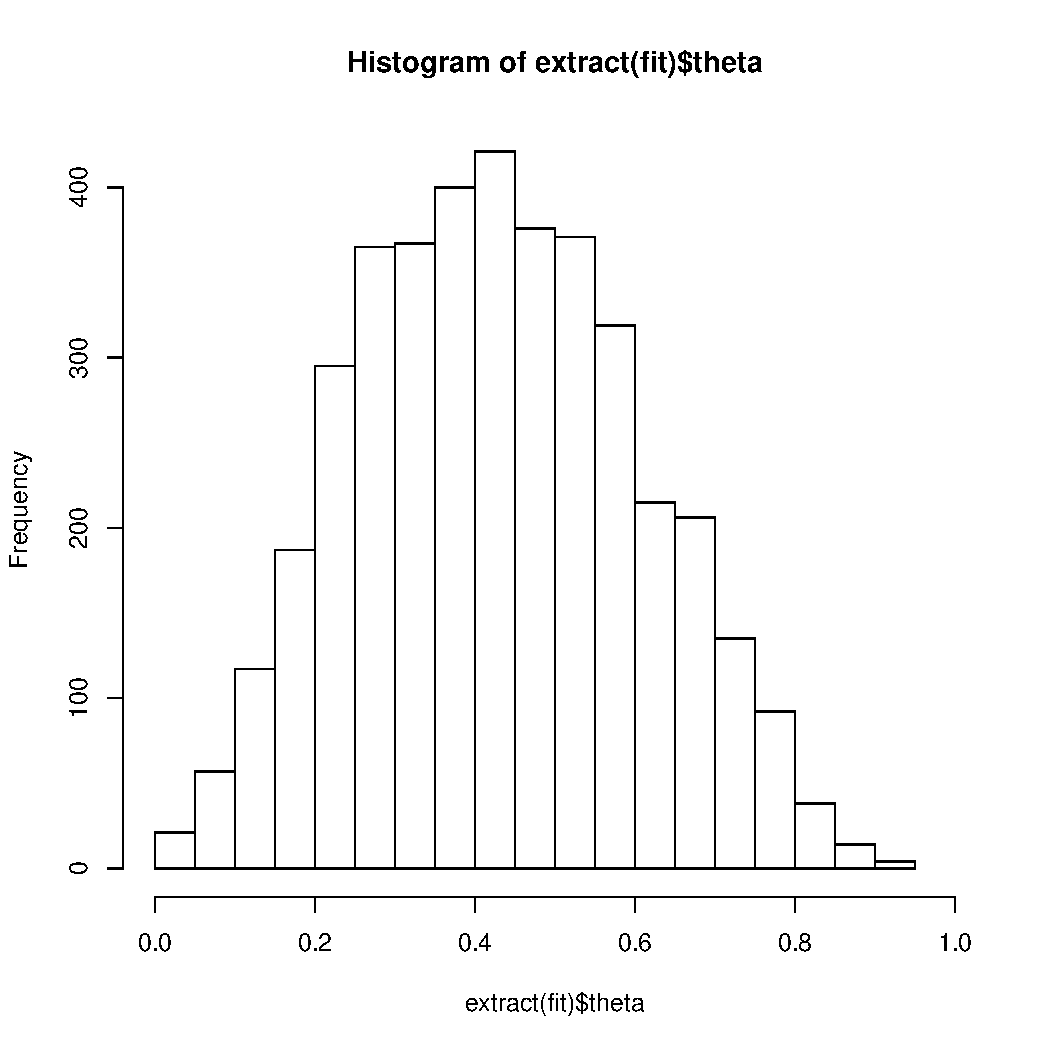
\includegraphics[height=0.9in]{img/bernoulli-posterior-histo.pdf}
\hspace*{24pt}
\end{minipage}


\sld{RStan:  Posterior Sample}
%
\begin{codein}
> theta_draws <- extract(fit)$theta;
> mean(theta_draws);
\end{codein}
\begin{codeout}
[1] 0.4128373
\end{codeout}
%
\begin{codein}
> quantile(theta_draws, probs=c(0.10, 0.90));
\end{codein}
\begin{codeout}
      10%       90%
0.2830349 0.5496858
\end{codeout}


\sld{Marginal Posterior Histograms}
%
\begin{codein}
theta_draws_df <- data.frame(list(theta = theta_draws));
plot <-
  ggplot(theta_draws_df, aes(x = theta)) +
  geom_histogram(bins=20, color = "gray");
plot;
\end{codein}
\vspace*{-9pt}
\begin{center}
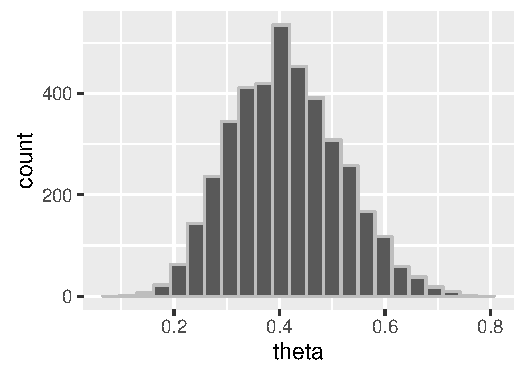
\includegraphics[height=1.25in]{img/bern-posterior-histogram.pdf}
\end{center}
\vspace*{-0.1in}
\begin{subitemize}
\item
Displays the full posterior {\slshape marginal} distribution $p(\theta \,
| \, y)$
\end{subitemize}



\sld{RStan: MAP, penalized MLE}
%
\begin{itemize}
\item Stan's optimization for estimation; two views:
\begin{subitemize}
\item max posterior mode, aka max a posteriori (MAP)
\item max penalized likelihood (MLE)
\end{subitemize}
\end{itemize}
\begin{center}
\begin{minipage}[t]{0.8\textwidth}\small
\begin{Verbatim}
> library(rstan);
> N <- 5;
> y <- c(0,1,1,0,0);
> model <- stan_model("bernoulli.stan");
> mle <- optimizing(model, data=c("N", "y"));
...
> print(mle, digits=2)
$par              $value  (log density)
theta             [1] -3.4
  0.4
\end{Verbatim}
\begin{subitemize}
\item Posterior: $\distro{Beta}(1+2, 1+3)$;  mode $0.40$; mean $0.43$
\item Density: MLE w/o Jacobian;  MCMC with Jacobian
\end{subitemize}
\end{minipage}
\end{center}


\sld{Plug in Posterior Draws}
%
\begin{itemize}
\item Extracting the posterior draws
\begin{codein}
> theta_draws <- extract(fit)$theta;
\end{codein}
\item Calculating posterior mean (estimator)
\begin{codein}
> mean(theta_draws);
\end{codein}
\begin{codeout}
[1] 0.4128373
\end{codeout}
\item Calculating posterior intervals
\begin{codein}
> quantile(theta_draws, probs=c(0.10, 0.90));
\end{codein}
\begin{codeout}
      10%       90%
0.2830349 0.5496858
\end{codeout}
\end{itemize}


\sld{ggplot2: Plotting}
%
\begin{codein}
theta_draws_df <- data.frame(list(theta = theta_draws));
plot <-
  ggplot(theta_draws_df, aes(x = theta)) +
  geom_histogram(bins=20, color = "gray");
plot;
\end{codein}
\vspace*{-9pt}
\begin{center}
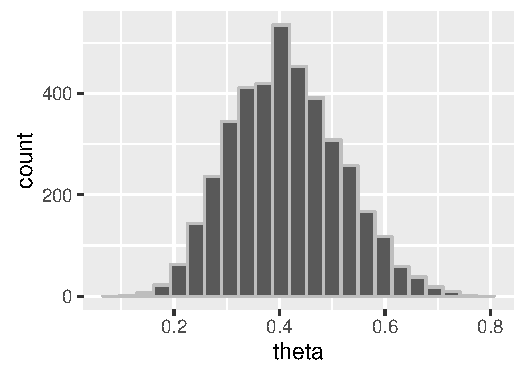
\includegraphics[height=1.45in]{img/bern-posterior-histogram.pdf}
\end{center}


\sld{Default Priors and Vectorization}
%
\begin{itemize}
\item All parameters are uniform by default
\item Probability functions can be vectorized (more efficient)
\item Thus
{\small
\begin{Verbatim}
      theta ~ uniform(0,1);
      for (n in 1:N)
        y[n] ~ bernoulli(theta);
\end{Verbatim}
}
\mbox{ }
\\
{\normalsize reduces to}
\\
{\small
\begin{Verbatim}
      y ~ bernoulli(theta);
\end{Verbatim}
}
\end{itemize}


\mypart{}{Male Birth Ratio}


\sld{Birth Rate by Sex}
\begin{itemize}
\item \myemph{Laplace}'s data on live births in Paris from 1745--1770:
\vspace*{-4pt}
\begin{center}\small
\begin{tabular}{c|c}
{\slshape sex} & {\slshape live births}
\\ \hline
female & 241\,945
\\
male & 251\,527
\end{tabular}
\end{center}
\item \myemph{Question 1} (Estimation)
\\
What is the birth rate of boys vs. girls?

\item \myemph{Question 2} (Event Probability)
\\
Is a boy more likely to be born than a girl?
%
\item Bayes (1763) set up the ``Bayesian'' model
\item Laplace (1781, 1786) solved for the posterior
\end{itemize}


\sld{Binomial Distribution}
%
\begin{itemize}
\item Binomial distribution is number of successes $y$ in $N$
i.i.d. Bernoulli trials with chance of success $\theta$
\item If $y_1,\ldots,y_N\sim \distro{Bernoulli}(\theta)$,
\\[4pt] then $(y_1 + \cdots + y_N) \sim \distro{Binomial}(N,\theta)$
\item The analytic form is
\[
\distro{Binomial}(y|N,\theta)
\ = \ \binom{N}{y} \theta^{y} (1 - \theta)^{N-y}
\]
where the binomial coefficient normalizes for permutations (i.e.,
which subset of $n$ has $y_n = 1$),
\[
\binom{N}{y} = \frac{N!}{y! \, (N-y)!}
\]
\end{itemize}


\sld{Binomial Distribution}
%
\begin{itemize}
\item Don't know order of births, only total.
\item If $y_1,\ldots,y_N\sim \distro{Bernoulli}(\theta)$,
\\[4pt] then $(y_1 + \cdots + y_N) \sim \distro{Binomial}(N,\theta)$
\item The analytic form is
\[
\distro{Binomial}(y|N,\theta)
\ = \ \binom{N}{y} \theta^{y} (1 - \theta)^{N-y}
\]
where the binomial coefficient normalizes for permutations (i.e.,
which subset of $n$ has $y_n = 1$),
\[
\binom{N}{y} = \frac{N!}{y! \, (N-y)!}
\]
\end{itemize}


\sld{Mathematics vs.\ Simulation}
%
\begin{itemize}
\item Luckily, we don't have to be as good at math as Laplace
\item Nowadays, we calculate all these integrals by computer using
  tools like Stan
\vfill
\begin{quote}\slshape
  If you wanted to do foundational research in statistics in the
  mid-twentieth century, you had to be bit of a mathematician, whether
  you wanted to or not. \ldots if you want to do statistical research
  at the turn of the twenty-first century, you have to be a computer
  programmer.  \\[3pt] \mbox{ } \hfill {\small ---from Andrew's blog}
\end{quote}
\end{itemize}


\sld{Bayes's Binomial Model}
%
\begin{itemize}
\item{Data}
\begin{subitemize}
\item $y$: total number of male live births (241,945)
\item $N$ : total number of live births (493,472)
\end{subitemize}
\item Parameter
\begin{subitemize}
\item $\theta \in (0,1)$: proportion of male live births
\end{subitemize}
\item Likelihood
\[
p(y|N,\theta)
\ = \ \distro{Binomial}(y|N,\theta)
\ = \ \binom{N}{y} \theta^{y} (1 - \theta)^{N-y}
\]
\item Prior
\[
p(\theta)
\ = \ \distro{Uniform}(\theta \, | \, 0,1)
\ = \ 1
\]
\end{itemize}





\sld{Beta Distribution}
%
\begin{itemize}
\item Required for analytic posterior of Bayes's model
\item For parameters $\alpha,\beta > 0$ and $\theta \in (0,1)$,
\[
\distro{Beta}(\theta|\alpha,\beta)
\ = \ \frac{1}{\Betafun(\alpha,\beta)}
      \theta^{\alpha - 1} \,
      (1 - \theta)^{\beta-1}
\]
\item Euler's Beta function is used to normalize,
\[
\Betafun(\alpha,\beta)
\ = \ \int_0^1 u^{\alpha-1}(1-u)^{\beta-1} du
\ = \ \frac{\Gamma(\alpha)\,\Gamma(\beta)}{\Gamma(\alpha + \beta)}
\]
where $\Gamma()$ is continuous generalization of factorial
\item Note: \ $\distro{Beta}(\theta|1,1) = \distro{Uniform}(\theta|0,1)$
\end{itemize}


\sld{Beta Distribution --- Examples}
%
\vspace*{-4pt}
\begin{itemize}
\item Unnormalized posterior density assuming uniform prior and $y$
  successes out of $n$ trials (all with mean 0.6).
\end{itemize}
\begin{center}
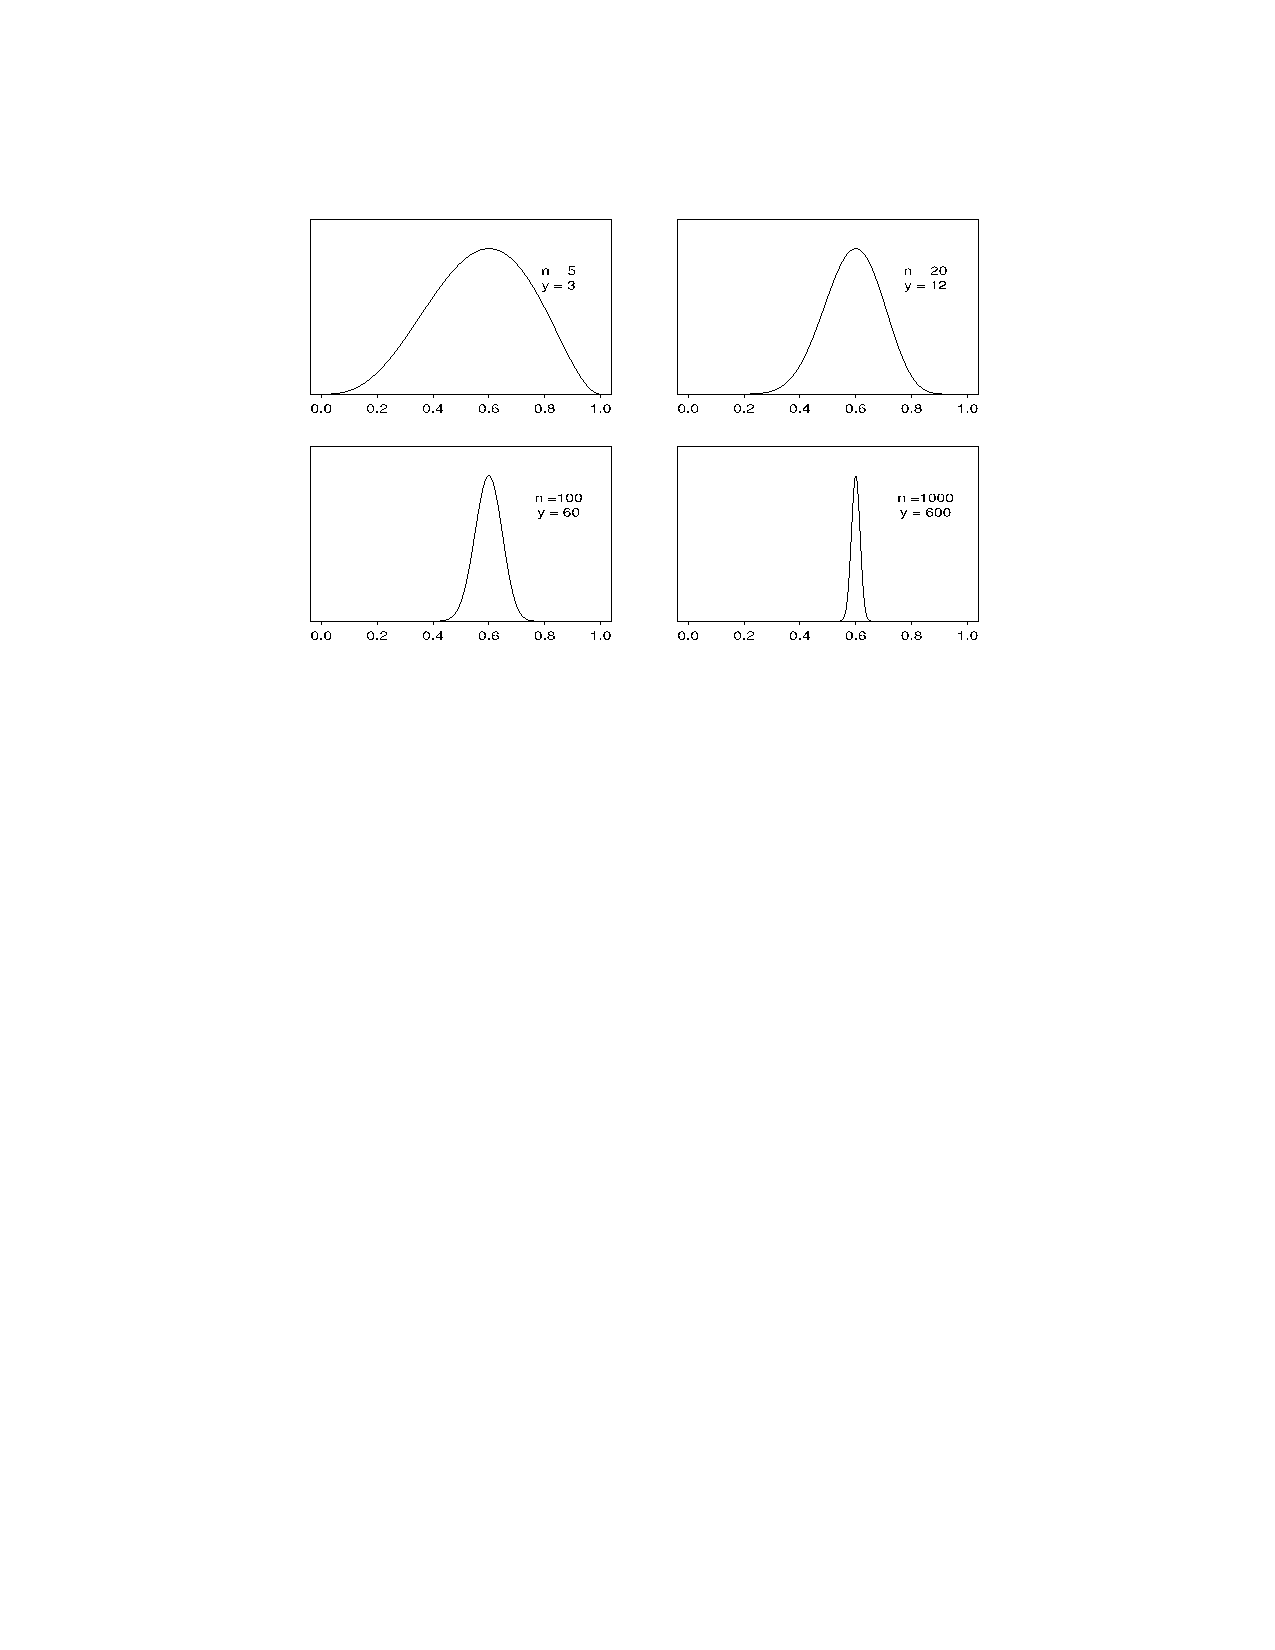
\includegraphics[height=1.6in]{img/bda-beta-plots.pdf}
\end{center}
\vspace*{-12pt}
\hfill {\tiny Gelman et al. (2013) {\slshape Bayesian Data Analysis},
  3rd Edition.}


\sld{Laplace Turns the Crank}
%
\begin{itemize}
\item Given Bayes's general formula for the posterior
\[
p(\theta|y,N)
\ = \
\frac{\distro{Binomial}(y|N,\theta) \, \distro{Uniform}(\theta|0,1)}
     {\int_{\Theta} \distro{Binomial}(y|N,\theta') \,  p(\theta')
       d\theta'}
\]
\item Laplace used Euler's Beta function (B) to normalize the
  posterior, with final solution
\[
p(\theta|y,N)
\ = \ \distro{Beta}(\theta \, | \, y + 1, \ N - y + 1)
\]
\end{itemize}


\sld{Laplace turns the Crank}
%
\begin{itemize}
\item What is probability that a male live birth is more probable?
\begin{eqnarray*}
\Prob{\theta > 0.5}
& = &  \int_{\Theta} \indicator{\theta > 0.5} \, p(\theta|y,N) d\theta
\\[4pt]
& = &  \int_{0.5}^1 p(\theta|y,N) d\theta
\\[4pt]
& \approx &  1 - 10^{-42}
\end{eqnarray*}
\item  Laplace solved Bayes's integral by
\begin{subitemize}
\item determing the posterior was a beta distribution (conjugacy!)
\item and solving the normalization (gamma functions)
\end{subitemize}
\end{itemize}


\sld{Calculating Laplace's Answers}
\begin{stancode}
transformed data {
  int male = 251527;
  int female = 241945;
}
parameters {
  real<lower=0, upper=1> theta;
}
model {
  male ~ binomial(male + female, theta);
}
generated quantities {
  int<lower=0, upper=1> theta_gt_half = (theta > 0.5);
}
\end{stancode}


\sld{And the Answer is...}
%
\begin{codein}
> fit <- stan("laplace.stan", iter=100000);
> print(fit, probs=c(0.005, 0.995), digits=3)
\end{codein}
\begin{codeout}
                    mean   0.5%  99.5%
theta               0.51  0.508  0.512
theta_gt_half       1.00  1.000  1.000
\end{codeout}
%
\begin{itemize}
\item Q1: $\theta$ is 99\% certain to lie in $(0.508, 0.512)$
%
\item Q2:  Laplace ``morally certain'' boys more prevalent
\end{itemize}


\sld{Estimation}
%
\begin{itemize}
\item Posterior is $\distro{Beta}(\theta \, | \, 1 + 241\,945, \ 1 + 251\,527)$
\item Posterior mean:
\[
\frac{1 + 241\,945}
     {1 + 241\,945 + 1 + 251\,527}
\approx 0.490291{\bf3}
\]
\item Maximum likelihood estimate same as posterior mode (because
  of uniform prior)
\[
\frac{241\,945}
     {241\,945 + 251\,527}
\approx 0.490291{\bf2}
\]
\item As number of observations approaches $\infty$,
\\
MLE approaches posterior mean
\end{itemize}


\sld{Event Probability Inference}
%
\begin{itemize}
\item What is probability that a male live birth is more likely than a
  female live birth?
\begin{eqnarray*}
\Prob{\theta > 0.5}
& = &  \int_{\Theta} \indicator{\theta > 0.5} \, p(\theta|y,N) d\theta
\\[4pt]
& = &  \int_{0.5}^1 p(\theta|y,N) d\theta
\\[4pt]
& = &  1 - F_{\theta|y,N}(0.5)
\\[4pt]
& \approx &  10^{-42}
\end{eqnarray*}
\item $\indicator{\phi} = 1$ if condition $\phi$ is true and 0 otherwise.
\item  $F_{\theta|y,N}$ is posterior cumulative distribution
function (cdf).
\end{itemize}


\mypart{}{Fisher "Exact" Test}


\sld{Bayesian ``Fisher Exact Test''}
%
\vspace*{-4pt}
\begin{itemize}
\item Suppose we observe the following data on handedness
\begin{center}
{\small
\begin{tabular}{c|c|c||c}
     & {\slshape sinister} & {\slshape dexter} & TOTAL
\\ \hline \hline
{\slshape male} & 9 ($y_1$) & 43 & 52 ($N_1$)
\\
{\slshape female} & 4 ($y_2$) & 44 & 48 ($N_2$)
\end{tabular}
}
\end{center}
\item Assume likelihoods $\distro{Binomial}(y_k|N_k,\theta_k)$, uniform
  priors
\item Are men more likely to be lefthanded?
{\small
\begin{eqnarray*}
\Prob{\theta_1 > \theta_2 \, | \, y, N}
& = &
\int_{\Theta} \indicator{\theta_1 > \theta_2} \, p(\theta|y,N) \,
d\theta
\\[4pt]
& \approx & \frac{1}{M} \sum_{m=1}^M \indicator{\theta_1^{(m)} > \theta_2^{(m)}}.
\end{eqnarray*}
}
\end{itemize}


\sld{Stan Binomial Comparison}
%
\begin{stancode}
data {
  int y[2];
  int N[2];
}
parameters {
  vector<lower=0,upper=1> theta[2];
}
model {
  y ~ binomial(N, theta);
}
generated quantities {
  real boys_minus_girls = theta[1] - theta[2];
  int boys_gt_girls = theta[1] > theta[2];
}
\end{stancode}


\sld{Binomial Comparison Results}
%
\begin{codeout}
                   mean    2.5%  97.5%
theta[1]           0.22    0.12   0.35
theta[2]           0.11    0.04   0.21
boys_minus_girls   0.12   -0.03   0.26
boys_gt_girls      0.93    0.00   1.00
\end{codeout}
\begin{itemize}
\item
$\mathrm{Pr}[\theta_1 > \theta_2 \,|\, y] \approx 0.93$
\item
$\mathrm{Pr}\left[
(\theta_1 - \theta_2) \in (-0.03, 0.26)
\,|\, y
\right]
\, = \, 95\%$
\end{itemize}


\sld{Visualizing Posterior Difference}
%
\begin{itemize}
\item Plot of posterior difference, $p(\theta_1 - \theta_2 \, | \, y,
  N)$ (men - women)
\begin{center}
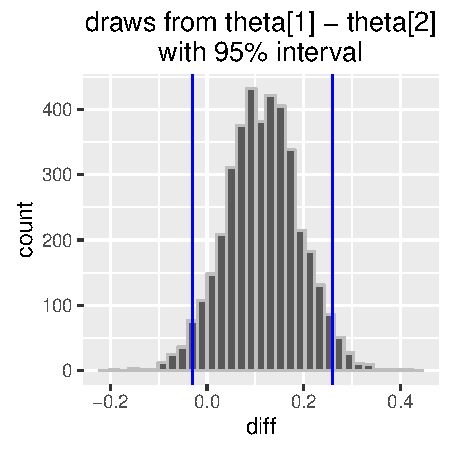
\includegraphics[height=1.65in]{img/lefty-posterior.pdf}
\end{center}
\item Vertical bars: central 95\% posterior interval $(-0.03,0.26)$
\end{itemize}


\mypart{}{More Stan Models}


\sld{Posterior Predictive Distribution}
%
\begin{itemize}
\item Predict new data ($\tilde{y}$) given observed data ($y$)
\item Includes two kinds of uncertainty
\begin{subitemize}
\item parameter estimation uncertainty: $p(\theta | y)$
\item sampling uncertainty:  $p(\tilde{y} | \theta)$
\end{subitemize}
\vspace*{-8pt}\begin{eqnarray*}
p(\tilde{y} |  y)
& = & \int p(\tilde{y} | \theta)
           \ p(\theta | y)
           \ \mathrm{d}\theta
\\[4pt]
& \approx & \frac{1}{M} \sum_{m=1}^M p(\tilde{y} | \theta^{(m)})
\end{eqnarray*}
\item Can generate predictions as sample of draws $\tilde{y}^{(m)}$
  based on $\theta^{(m)}$
\end{itemize}


\sld{Posterior Predictive Inference}
%
\begin{itemize}
\item Parameters $\theta$, observed data $y$, and data to predict $\tilde{y}$
\[
p(\tilde{y}|y) = \int_{\Theta} p(\tilde{y}|\theta) \ p(\theta|y) \ d\theta
\]
\item
{\small
\begin{Verbatim}
data {
  int<lower=0> N_tilde;
  matrix[N_tilde,K] x_tilde;
  ...
parameters {
  vector[N_tilde] y_tilde;
  ...
model {
  y_tilde ~ normal(x_tilde * beta, sigma);
\end{Verbatim}
}
\end{itemize}


\sld{Predict w.\ Generated Quantities}
%
\begin{itemize}
\item Replace sampling with pseudo-random number generation
{\footnotesize
\begin{Verbatim}
   generated quantities {
     vector[N_tilde] y_tilde;

     for (n in 1:N_tilde)
       y_tilde[n] <- normal_rng(x_tilde[n] * beta, sigma);
   }
\end{Verbatim}
}
\item Must include noise for predictive uncertainty
\item PRNGs only allowed in generated quantities block
\begin{subitemize}
\item more computationally efficient per iteration
\item more statistically efficient with i.i.d.\ samples \\
(i.e., MC, not MCMC)
\end{subitemize}
\end{itemize}


\sld{Linear Regression with Prediction}
%
\begin{stancode}
data {
  int<lower=0> N;               int<lower=0> K;
  matrix[N, K] x;               vector[N] y;
  matrix[N_tilde, K] x_tilde;
}
parameters {
  vector[K] beta;               real<lower=0> sigma;
}
model {
  y ~ normal(x * beta, sigma);
}
generated quantities {
  vector[N_tilde] y_tilde
    = normal_rng(x_tilde * beta, sigma);
}
\end{stancode}


\sld{Transforming Precision to Scale}
%
\begin{stancode}
    parameters {
      real<lower=0> tau;
      ...
    }
    transformed parameters {
      real<lower=0> sigma = tau^(-0.5);
    }
\end{stancode}


\sld{Transforms: Non-Centered Parameterization}
{\small
\begin{Verbatim}
parameters {
  vector[K] beta_std;  // non-centered
}
transformed parameters {
  vector[K] beta =  mu + sigma * beta_std;
}
model {
  // implies:  beta ~ normal(mu, sigma)
  beta_std ~ normal(0, 1);
}
\end{Verbatim}
}


\sld{Logistic Regression}
%
\begin{stancode}
     data {
       int<lower=1> K;
       int<lower=0> N;
       matrix[N,K] x;
       int<lower=0,upper=1> y[N];
     }
     parameters {
       vector[K] beta;
     }
     model {
        beta ~ cauchy(0, 2.5);          // prior
        y ~ bernoulli_logit(x * beta);  // likelihood
     }
\end{stancode}


\sld{Generalized Linear Models}
%
\begin{itemize}
\item Direct parameterizations more efficient and stable
\item \myemph{Logistic regression} (boolean/binary data)
\begin{subitemize}
\item \Verb|y ~ bernoulli(inv_logit(eta));|
\item \Verb|y ~ bernoulli_logit(eta);|
\item Probit via \code{Phi} (normal cdf)
\item Robit (robust) via Student-$t$ cdf
\end{subitemize}
\item \myemph{Poisson regression} (count data)
\begin{subitemize}
\item \Verb|y ~ poisson(exp(eta));|
\item \Verb|y ~ poisson_log(eta);|
\item Overdispersion with negative binomial
\end{subitemize}
\end{itemize}


\sld{GLMS, continued}
%
\begin{itemize}
\item \myemph{Multi-logit regression} (categorical data)
\begin{subitemize}
\item \Verb|y ~ categorical(softmax(eta));|
\item \Verb|y ~ categorical_logit(eta);|
\end{subitemize}
\item \myemph{Ordinal logistic regression} (ordered data)
\begin{subitemize}
\item Add cutpoints \code{c}
\item \Verb|y ~ ordered_logistic(eta, c);|
\end{subitemize}
\item \myemph{Robust linear regression} (overdispersed noise)
\begin{subitemize}
\item \Verb|y ~ student_t(nu, eta, sigma);|
\end{subitemize}
\end{itemize}


\sld{Time Series Autoregressive: AR(1)}
%
\begin{stancode}
  data {
    int<lower=0> N;   vector[N] y;
  }
  parameters {
    real alpha;  real beta;  real sigma;
  }
  model {
    y[2:n] ~ normal(alpha + beta * y[1:(n-1)], sigma);
  }
\end{stancode}


\sld{LKJ Density and Cholesky Factors}
%
\begin{itemize}
\item Density on \emph{correlation} \ matrices $\Omega$
%
\item $\distro{LKJCorr}(\Omega \, | \, \nu)
       \propto \mbox{det}(\Omega)^{(\nu - 1)}$
\begin{subitemize}
\item $\nu = 1$ uniform
\item $\nu > 1$ concentrates around unit matrix
\end{subitemize}
%
\item Work with Cholesky factor $L_{\Omega}$ s.t. $\Omega = L_{\Omega} \, L_{\Omega}^{\top}$
\begin{subitemize}
\item Density: $\distro{LKJCorrCholesky}(L_{\Omega} \, | \, \nu)
\propto |J| \, \mbox{det}(L_{\Omega} \, L_{\Omega}^{\top})^{(\nu - 1)}$
\item Jacobian adjustment for Cholesky factorization
\end{subitemize}
%
\end{itemize}
\vfill
\hfill {\footnotesize Lewandowski, Kurowicka, and Joe (2009)}


\sld{Covariance Random-Effects Priors}
%
\vspace*{-4pt}
{\footnotesize
\begin{Verbatim}
    parameters {
      vector[2] beta[G];
      cholesky_factor_corr[2] L_Omega;
      vector<lower=0>[2] sigma;

    model {
      sigma ~ cauchy(0, 2.5);
      L_Omega ~ lkj_cholesky(4);
      beta ~ multi_normal_cholesky(rep_vector(0, 2),
                             diag_pre_multiply(sigma, L_Omega));
      for (n in 1:N)
        y[n] ~ bernoulli_logit(... + x[n] * beta[gg[n]]);
\end{Verbatim}
}
\vspace*{6pt}
\begin{subitemize}
\item $G$ groups with varying slope and intercept; \code{gg} indicates group
\end{subitemize}


\sld{Multivariate Random-Effects Priors}
%
\begin{stancode}
parameters {
  vector[2] beta[G];
  cholesky_factor_corr[2] L_Omega;
  vector<lower=0>[2] sigma;
  ...
model {
  sigma ~ cauchy(0, 2.5);
  L_Omega ~ lkj_cholesky(4);
  beta ~ multi_normal_cholesky(rep_vector(0, 2),
                         diag_pre_multiply(sigma, L_Omega));
  for (n in 1:N)
    y[n] ~ bernoulli_logit(... + x[n] * beta[gg[n]]);
\end{stancode}


\sld{\large Example: Gaussian Process Estimation}
%
\vspace*{-5pt}
\begin{stancode}
data {
  int<lower=1> N;  vector[N] x; vector[N] y;
} parameters {
  real<lower=0> eta_sq, inv_rho_sq, sigma_sq;
} transformed parameters {
  real<lower=0> rho_sq; rho_sq <- inv(inv_rho_sq);
} model {
  matrix[N,N] Sigma;
  for (i in 1:(N-1)) {
    for (j in (i+1):N) {
      Sigma[i,j] <- eta_sq * exp(-rho_sq * square(x[i] - x[j]));
      Sigma[j,i] <- Sigma[i,j];
  }}
  for (k in 1:N) Sigma[k,k] <- eta_sq + sigma_sq;
  eta_sq, inv_rho_sq, sigma_sq ~ cauchy(0,5);
  y ~ multi_normal(rep_vector(0,N), Sigma);
}
\end{stancode}


\sld{\large Gaussian Process Predictions}
%
\begin{itemize}
\item Add predictors \code{x\_tilde[M]} for points to predict
\item Declare predicted values \code{y\_tilde[M]} as unconstrained parameters
\item Define \code{Sigma[M+N,M+N]} in terms of full \code{append\_row(x, x\_tilde)}
\item Model remains the same
{\small
\begin{Verbatim}
 append_row(y,y_tilde)
   ~ multi_normal(rep(0,N+M),Sigma);
\end{Verbatim}
}
\end{itemize}


\sld{Non-Centered Parameterization}
%
\begin{stancode}
parameters {
  vector[K] beta_std;  // non-centered
  real mu;
  real<lower=0> sigma;
}
transformed parameters {
  vector[K] beta = mu + sigma * beta_raw;
}
model {
  mu ~ cauchy(0, 2.5);
  sigma ~ cauchy(0, 2.5);
  beta_std ~ normal(0, 1);
}
\end{stancode}


\sld{Mixture of Two Normals}
%
{\footnotesize
\begin{Verbatim}
        for (n in 1:N) {
          real lp1;  real lp2;

          lp1 <- bernoulli_log(0, lambda)
                   + normal_log(y[n], mu[1], sigma[1]);

          lp2 <- bernoulli_log(1, lambda)
                   + normal_log(y[n], mu[2], sigma[2]);

          increment_log_prob(log_sum_exp(lp1,lp2));
\end{Verbatim}
}
\vspace*{2pt}
\begin{subitemize}
\item local variables reassigned; direct increment of log posterior
\item $\mbox{\rm log\_sum\_exp}(\alpha,\beta) = \log (\exp(\alpha) + \exp(\beta))$
\item \myemph{Much more efficient} than sampling (Rao-Blackwell Theorem)
\vspace*{10pt}
\end{subitemize}


\sld{Other Mixture Applications}
%
\begin{itemize}
\item Other multimodal data
\item Zero-inflated Poisson or hurdle models
\item Model comparison or mixture
\item Discrete change-point model
\item Hidden Markov model, Kalman filter
\item Almost anything with latent discrete parameters
\hfill
\item Other than variable choice, e.g., regression predictors
\begin{subitemize}
\item marginalization is exponential in number of vars
\end{subitemize}
\end{itemize}


\sld{Dynamic Systems with Diff Eqs}
%
\begin{itemize}
\item Simple harmonic oscillator
{\small
\begin{equation*}
\frac{d}{dt} y_1 = -y_2
\hspace*{0.5in}
\frac{d}{dt} y_2 = -y_1 - \theta y_2
\end{equation*}
}
\item Code as a function in Stan
\end{itemize}
{\footnotesize
\begin{Verbatim}
        functions {
          real[] sho(real t, real[] y, real[] theta,
                     real[] x_r, int[] x_i) {
            real dydt[2];
            dydt[1] <- y[2];
            dydt[2] <- -y[1] - theta[1] * y[2];
            return dydt;
          }
        }
\end{Verbatim}
}


\sld{Fit Noisy State Measurements}
%
{\footnotesize
\begin{Verbatim}
    data {
      int<lower=1> T;      real y[T,2];
      real t0;             real ts[T];
    }
    parameters {
      real y0[2];                // unknown initial state
      real theta[1];             // rates for equation
      vector<lower=0>[2] sigma;  // measurement error
    }
    model {
      real y_hat[T,2];
      ...priors...
      y_hat <- integrate_ode(sho, y0, t0, ts, theta, x_r, x_i);
      for (t in 1:T)
        y[t] ~ normal(y_hat[t], sigma);
    }
\end{Verbatim}
}



\mypart{}{Hierarchical Models}


\sld{Baseball At-Bats}
%
\begin{itemize}
\item For example, consider baseball batting ability.
\begin{subitemize}
\item
{\footnotesize Baseball is sort of like cricket, but with round bats, a
  one-way field, stationary ``bowlers'', four bases, short games,
  and no draws}
\end{subitemize}
\item Batters have a number of ``at-bats'' in a season, out of which they
  get a number of ``hits'' (hits are a good thing)
\item Nobody with higher than 40\% success rate since 1950s.
\item No player (excluding ``bowlers'') bats much less than 20\%.
\item Same approach applies to hospital pediatric surgery
  complications (a BUGS example), reviews on Yelp,
  test scores in multiple classrooms, \ldots
\end{itemize}


\sld{Baseball Data}
%
\\
\begin{minipage}[t]{0.49\textwidth}
\small
\begin{itemize}
\item Hits vs.\ at bats for 2006 AL (no bowlers); line at average
\item not much variation
\item variation related to number of trials
\item success rate increases with number of trials
\begin{subitemize}
\item at bats predictively in nuanced models
\item blue is pooled average, red is +/- 2
  binomial std devs
\end{subitemize}
\end{itemize}
\end{minipage}
%
\begin{minipage}[t]{0.50\textwidth}
\begin{center}
\vspace*{-36pt}
\hfill 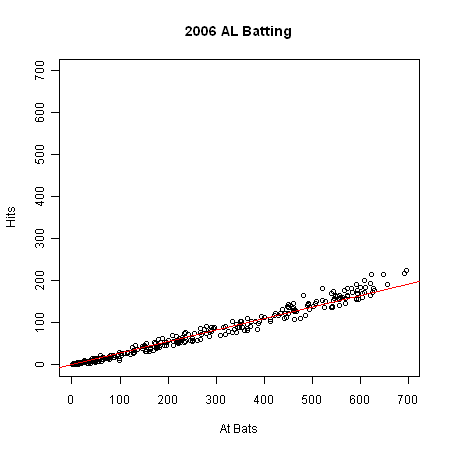
\includegraphics[height=1.1in]{img/al06hitsvsatbats.png}
\\[-18pt]
\hfill 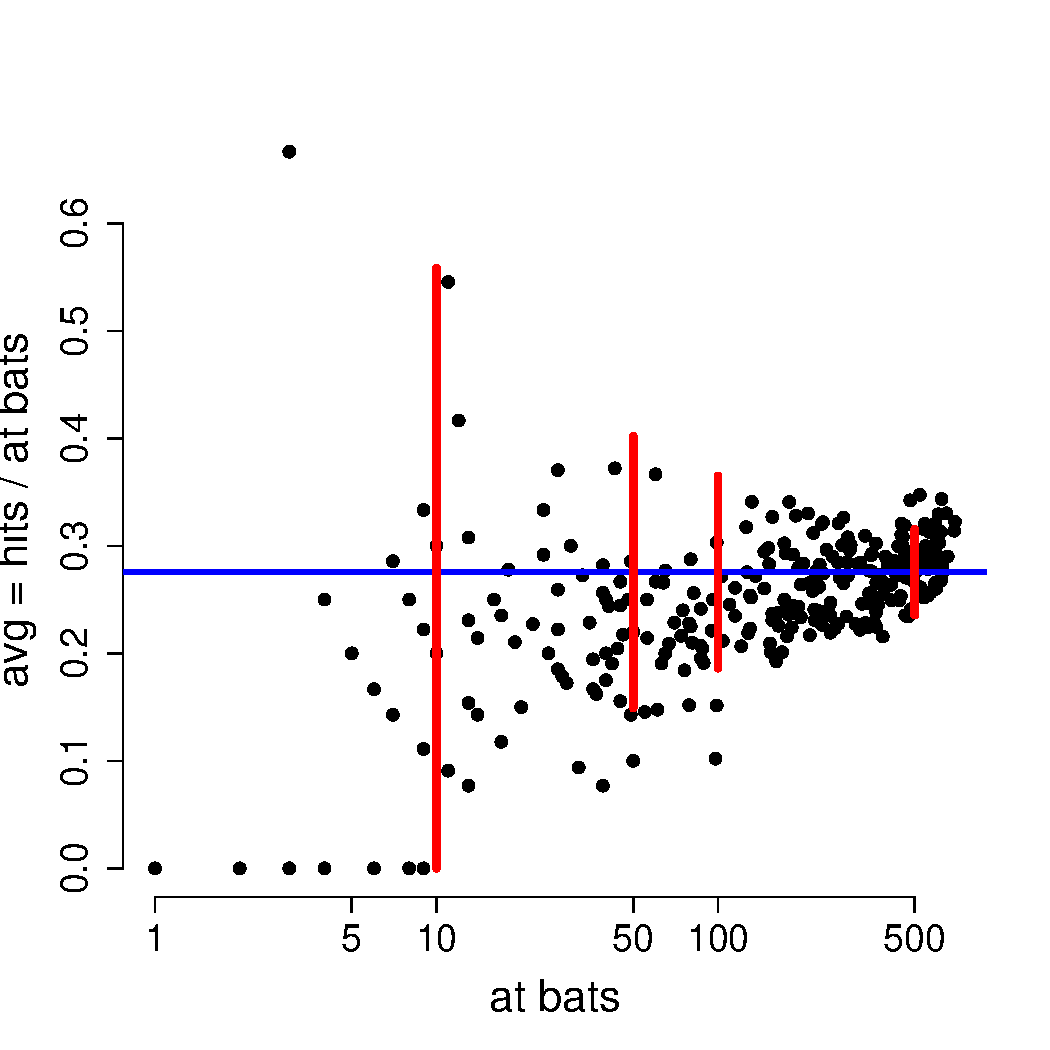
\includegraphics[height=1.65in]{img/bball-eda.pdf}
\end{center}
\end{minipage}


\sld{Pooling Data}
%
\begin{itemize}
\item How do we estimate the ability of a player who we observe
  getting 6 hits in 10 at-bats?  Or 0 hits in 5 at-bats?  Estimates of
  60\% or 0\% are absurd!
\item Same logic applies to players with 40 hits in 131 at bats or 152 hits in 537.
\item \emph{No pooling}: estimate each player separately
\item \emph{Complete pooling}: estimate all players together (assume no difference
  in abilities)
\item \emph{Partial pooling}: somewhere in the middle
\begin{subitemize}
\item use information about other players (i.e., the population)
to estimate a player's ability
\end{subitemize}
\end{itemize}


\sld{Complete Pooling Model in Stan}
%
\begin{subitemize}
\item Assume players all have same ability
\item Assume uniform prior on abilities
\begin{stancode}
data {
  int<lower=0> N;              // items
  int<lower=0> K[N];           // trials
  int<lower=0> y[N];           // successes
}
parameters {
  real<lower=0, upper=1> phi;  // chance of success
}
model {
  y ~ binomial(K, phi);        // vectorized likelihood
}
\end{stancode}
\end{subitemize}


\sld{No Pooling Model in Stan}
%
\begin{subitemize}
\item Assume each player has independent ability
\item Assume uniform priors on abilities
\begin{stancode}
data {
  int<lower=0> N;
  int<lower=0> K[N];
  int<lower=0> y[N];
}
parameters {
  real<lower=0, upper=1> phi[N];
}
model {pp
  y ~ binomial(K, phi);  // now y[n] matches phi[n]
}
\end{stancode}
\end{subitemize}


\sld{Hierarchical Models}
%
\begin{itemize}
\item Hierarchical models are principled way of determining how much
  pooling to apply.
\item Pull estimates toward the population mean based on amount of
  variation in population
\begin{subitemize}
\item low variance population: more pooling
\item high variance population: less pooling
\end{subitemize}
\item In limit
\begin{subitemize}
\item as variance goes to 0, get complete pooling
\item as variance goes to $\infty$, get no pooling
\end{subitemize}
\end{itemize}


\sld{Hierarchical Batting Ability}
%
\begin{itemize}
\item Instead of fixed priors, estimate priors along with other parameters
\item Still only uses data once for a single model fit
\item Data: $y_n, K_n$: hits, at-bats for player $n$
\item Parameters: $\phi_n$: ability for player $n$
\item Hyperparameters: $\alpha, \beta$: population mean and variance
\item Hyperpriors: fixed priors on $\alpha$ and $\beta$ (hardcoded)
\end{itemize}


\sld{Hierarchical Batting Model {\small (cont.)}}
%
\begin{eqnarray*}
\theta &  \sim & \distro{Uniform}(0,1)
\\[4pt]
\kappa & \sim & \distro{Pareto}(1.5)
\\[4pt]
\phi_n & \sim & \distro{Beta}(\kappa, \theta, \ \kappa \, (1 - \theta))
\\[4pt]
y_n & \sim & \distro{Binomial}(K_n, \phi_n)
\end{eqnarray*}
\begin{itemize}
\item Pareto provides power law distro on prior count:
{\small
\[
\distro{Pareto}(u \, | \, \alpha)
\ \propto \
\frac{\alpha}
     {u^{\alpha + 1}}
\]
}
\item $\theta$ is prior mean; \ $\kappa$ is prior count (plus 2).
\item Should use more informative prior on $\theta$.
\end{itemize}


\sld{Partial Pooling Model in Stan}
%
\begin{stancode}
data {
  int<lower=0> N;
  int<lower=0> K[N];
  int<lower=0> y[N];
}
parameters {
  real<lower=0, upper=1> theta;
  real<lower=0> kappa;
  vector<lower=0, upper=1>[N] phi;
}
model {
  kappa ~ pareto(1, 1.5);             // hyperprior
  theta ~ beta(kappa * theta,         // prior
               kappa * (1 - theta));
  y ~ binomial(K, theta);             // likelihood
}
\end{stancode}


\sld{Posterior for Hyperpriors}
%
\\[8pt]
\begin{minipage}[t]{0.55\textwidth}
\begin{itemize}
\item Scatterplot of draws
\item Crosshairs at mean
\item $\kappa = \alpha +
  \beta$ \ and \ $\theta = \frac{\alpha}{\alpha + \beta}$
\item Prior mean est: $\hat{\theta} = 0.271$
\item Prior count est: $\hat{\kappa} = 400$
\item Together yield prior std dev of only 0.022
\end{itemize}
\end{minipage}
\begin{minipage}[t]{0.45\textwidth}
\vfill
\mbox{ } \ \ \ \ \ \ 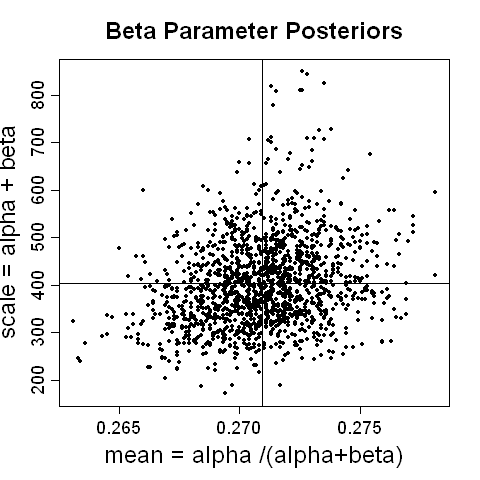
\includegraphics[height=1.4in]{img/baseball-beta-posterior-scatter.png}
\vfill
\end{minipage}


\sld{Posterior Ability {\normalsize (High Avg Players)}}
%
\vspace*{-8pt}
\begin{center}
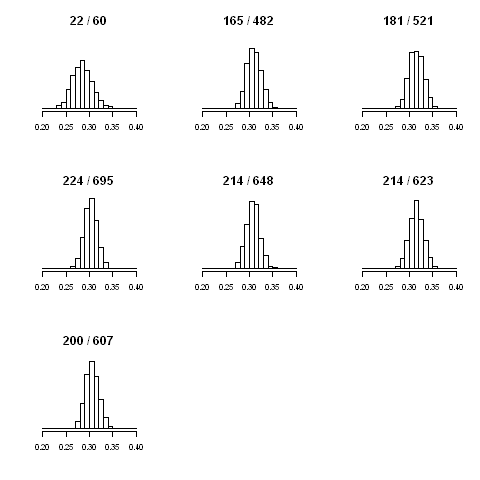
\includegraphics[height=2.25in]{img/batting-ability-posteriors.png}
\end{center}


\sld{Who's the Best?}
%
\vspace*{-2pt}\small
\begin{itemize}
\item Posterior probability that player $n$ has highest ability:
\[
\mbox{Pr}[\phi_n \geq \max(\phi) \, | \, y]
\]
\item Code up with indicator variable in Stan
\begin{stancode}
generated quantities {
  int<lower=0, upper=1> is_best[N];
  for (n in 1:N)
    is_best[n] <- (phi[n] >= max(phi));
}
\end{stancode}
\end{itemize}


\sld{Multiple Comparisons}
%
\begin{itemize}
\item Hierarchical model \myemph{adjusts for multiple comparisons} by pulling
  all estimates toward population mean
\end{itemize}


\sld{Results for 2006 AL Season}
%
\begin{center}
{\small
\begin{tabular}{rrrr}
\emph{Player} & \emph{Average} & \emph{At-Bats} & $\Prob{\text{best}}$
\\ \hline
Mauer & .347 & 521 & 0.12
\\
Jeter & .343 & 623 & 0.11
\\
& .342 & 482 & 0.08
\\
& .330 & 648 & 0.04
\\
& .330 & 607 & 0.04
\\
& .367 & 60 & 0.02
\\
& .322 & 695 & 0.02
\end{tabular}
}
\end{center}
\begin{itemize}
\item Posterior probabilities reflect uncertainty in data
\item {\footnotesize In last game (of 162), Mauer (Minnesota) edged out Jeter (NY)}
\end{itemize}


\sld{Efron \& Morris (1975) Data}
%
\begin{itemize}
\item From their classic analysis for shrinkage/empirical Bayes
\item Picked batters with 45 at bats on a given day (artificial!)
\end{itemize}
\begin{stancode}
   FirstName   LastName Hits At.Bats Rest.At.Bats Rest.Hits
1    Roberto   Clemente   18      45          367       127
2      Frank   Robinson   17      45          426       127
3      Frank     Howard   16      45          521       144
4        Jay  Johnstone   15      45          275        61
5        Ken      Berry   14      45          418       114
6        Jim    Spencer   14      45          466       126
7        Don  Kessinger   13      45          586       155
8       Luis   Alvarado   12      45          138        29
9        Ron      Santo   11      45          510       137
10       Ron    Swaboda   11      45          200        46
11      Rico Petrocelli   10      45          538       142
\end{stancode}


\sld{Pooling vs. No-Pooling Estimates}
%
\vspace*{-0.15in}
\begin{center}
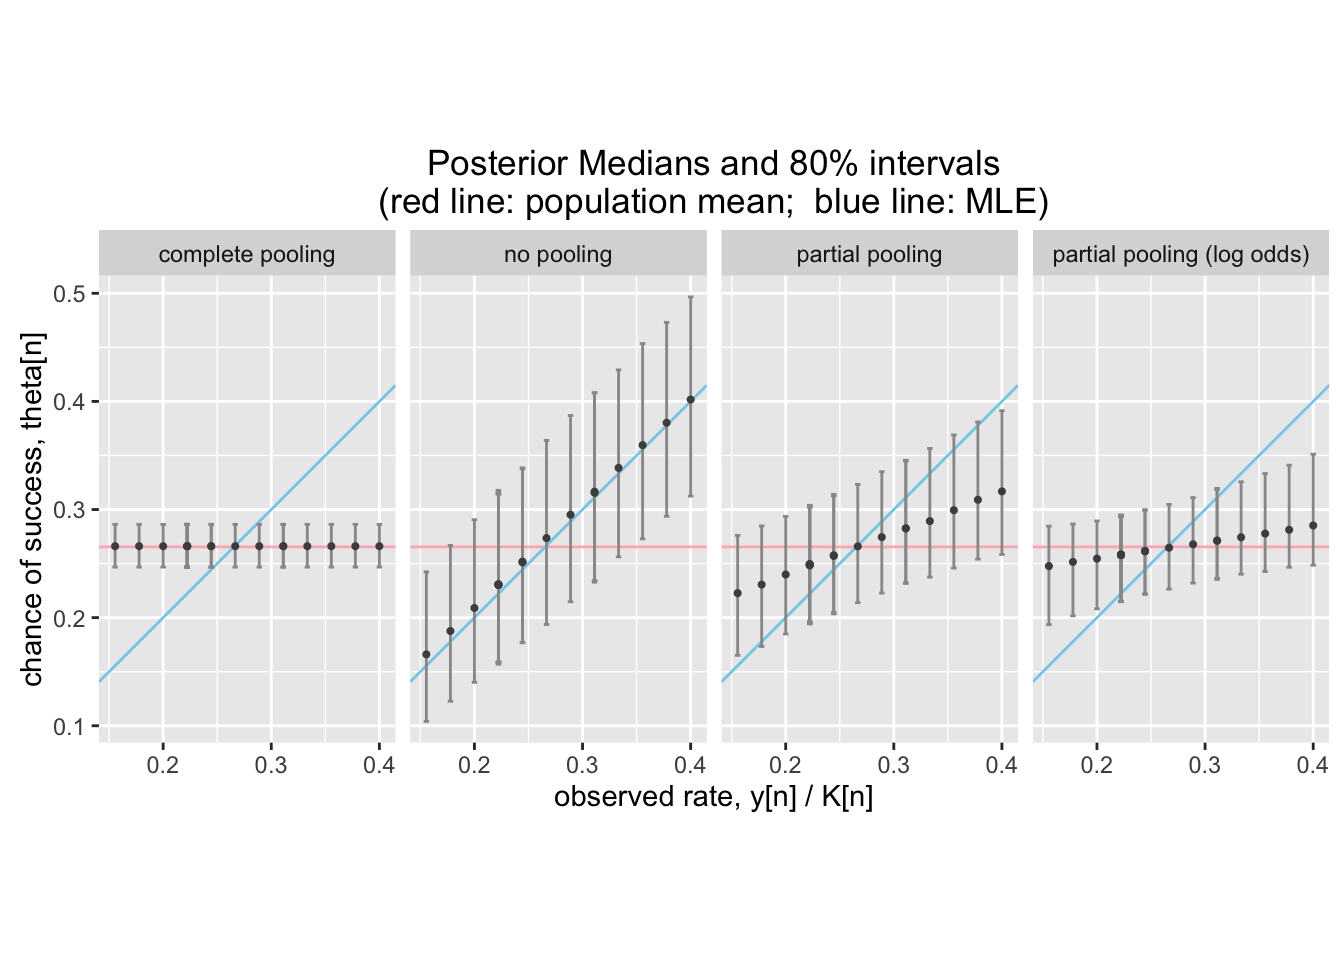
\includegraphics[height=2.25in]{img/pool-no-pool.png}
\end{center}
\vspace*{-0.35in}
\begin{subitemize}
\item complete pooling, no pooling, partial pooling, (log odds)
\end{subitemize}

\sld{Ranking}
\begin{stancode}
generated quantities {
  int<lower=1, upper=N> rnk[N];      // rank of player n
  {
    int dsc[N];
    dsc <- sort_indices_desc(theta);
    for (n in 1:N)
      rnk[dsc[n]] <- n;
  }
\end{stancode}


\sld{Posterior Ranks}
%
\begin{center}
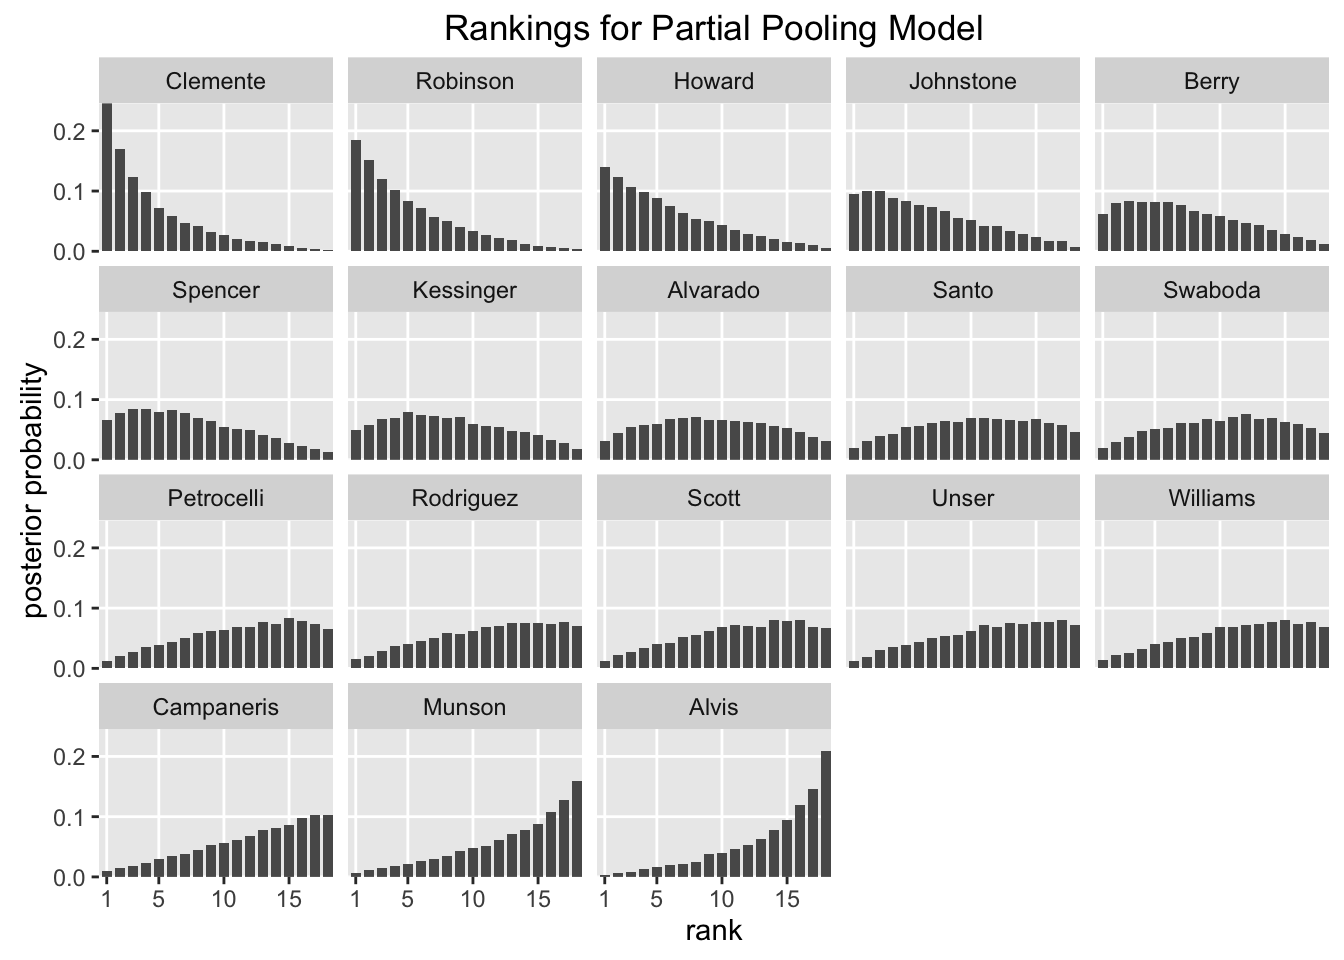
\includegraphics[height=2.0in]{img/rankings-pool.png}
\end{center}

\sld{Who is Best? {\normalsize better Stan code}}
\begin{stancode}
generated quantities {
  ...
  int<lower=0, upper=1> is_best[N];
  ...
  for (n in 1:N)
    is_best[n] <- (rnk[n] == 1);  // more efficient
  ...
\end{stancode}

\sld{Who is Best? Posterior}
\begin{center}
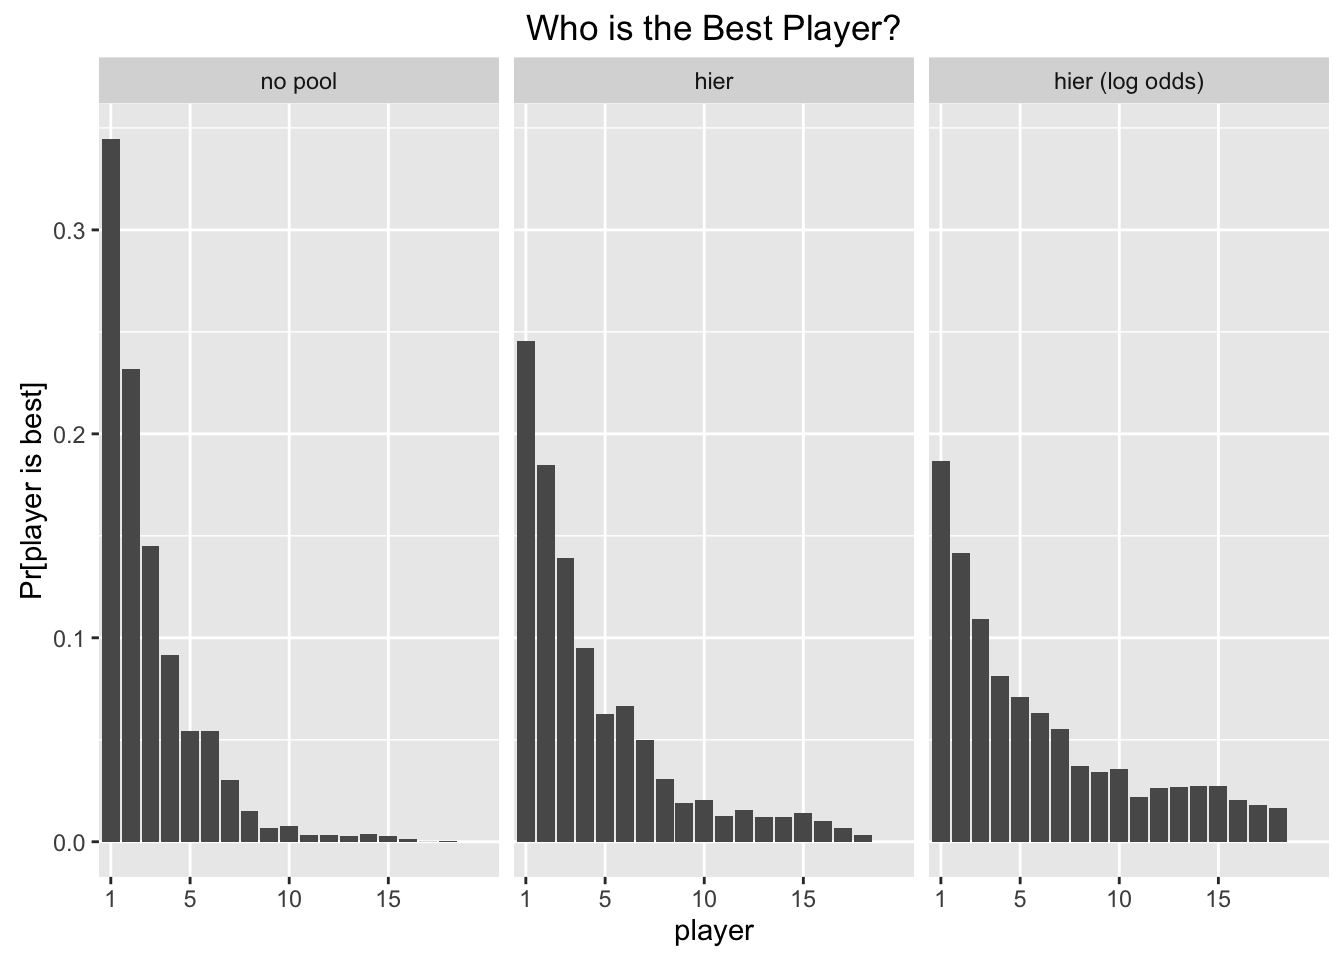
\includegraphics[height=2.0in]{img/who-is-best.png}
\end{center}


\sld{Posterior Predictive Inference}
%
\begin{itemize}
\item How do we predict new outcomes (e.g., rest of season)?
\begin{stancode}
data {
  int<lower=0> K_new[N];       // new trials
  int<lower=0> y_new[N];       // new successes
  ...
generated quantities {
  int<lower=0> z[N];  // posterior prediction
  for (n in 1:N)
    z[n] <- binomial_rng(K_new[n], theta[n]);
\end{stancode}
\item Full Bayes accounts for two sources of uncertainty
\begin{subitemize}
\item estimation uncertainty (built into posterior)
\item sampling uncertainty (explicit RNG function)
\end{subitemize}
\end{itemize}

\sld{Posterior Predictions}
\begin{center}
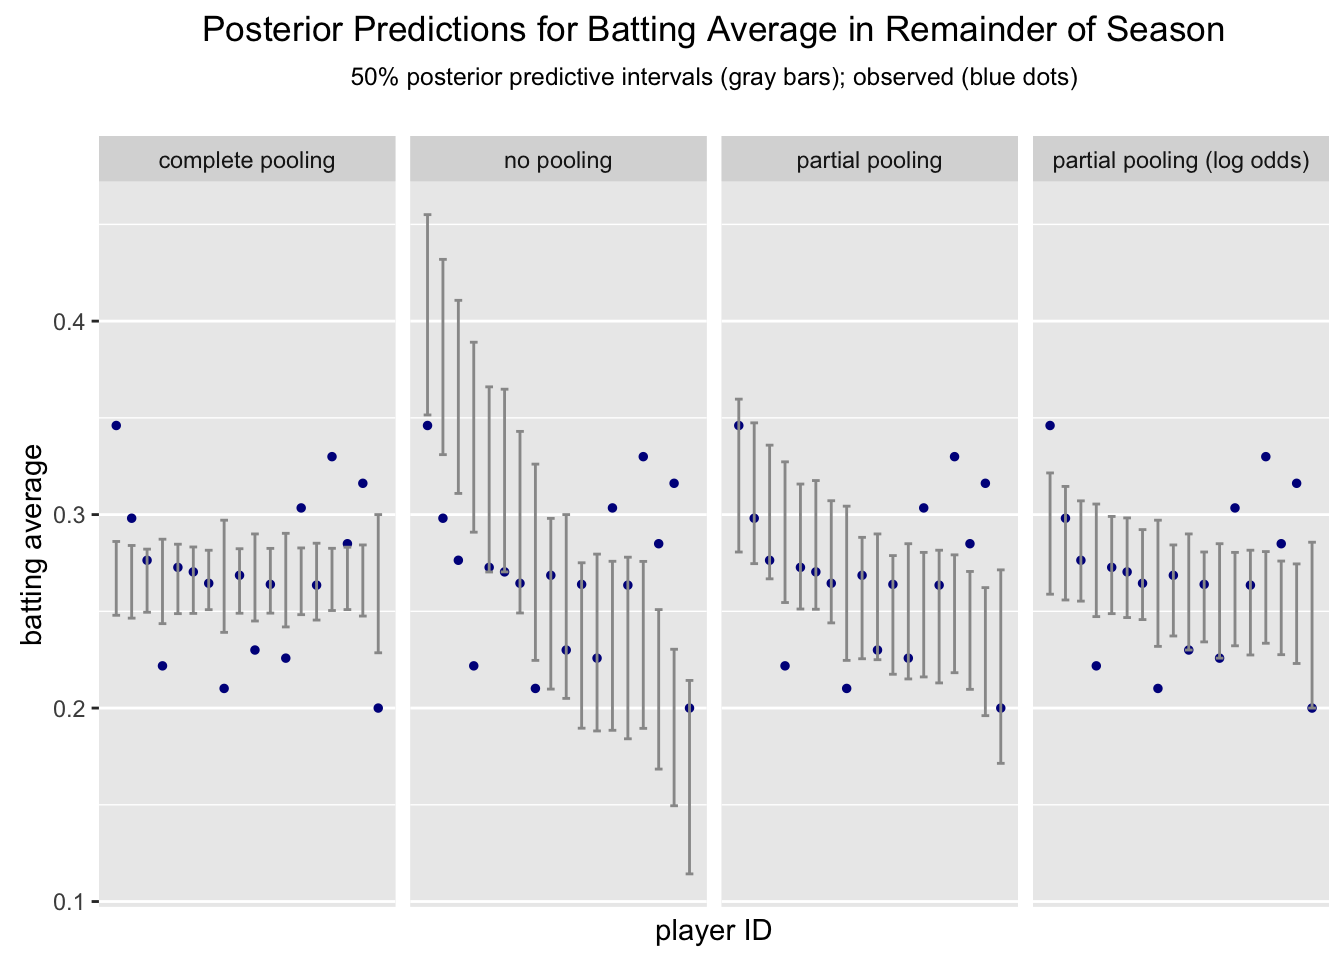
\includegraphics[height=2in]{img/posterior-predictions.png}
\end{center}


\sld{Posterior Predictive Check}
%
\begin{itemize}
\item Replicate data from paraemters
\end{itemize}
\begin{stancode}
generated quantities {
  ...
  for (n in 1:N)
    y_rep[n] <- binomial_rng(K[n], theta[n]);
  for (n in 1:N)
    y_pop_rep[n] <- binomial_rng(K[n],
                                 beta_rng(phi * kappa,
                                          (1 - phi) * kappa));
  min_y_rep <- min(y_rep);
  sd_y_rep <- sd(to_vector(y_rep));
  p_min <- (min_y_rep >= min_y);
  p_sd <- (sd_y_rep >= sd_y);
}
\end{stancode}

\sld{Posterior $p$-Values}
\begin{center}
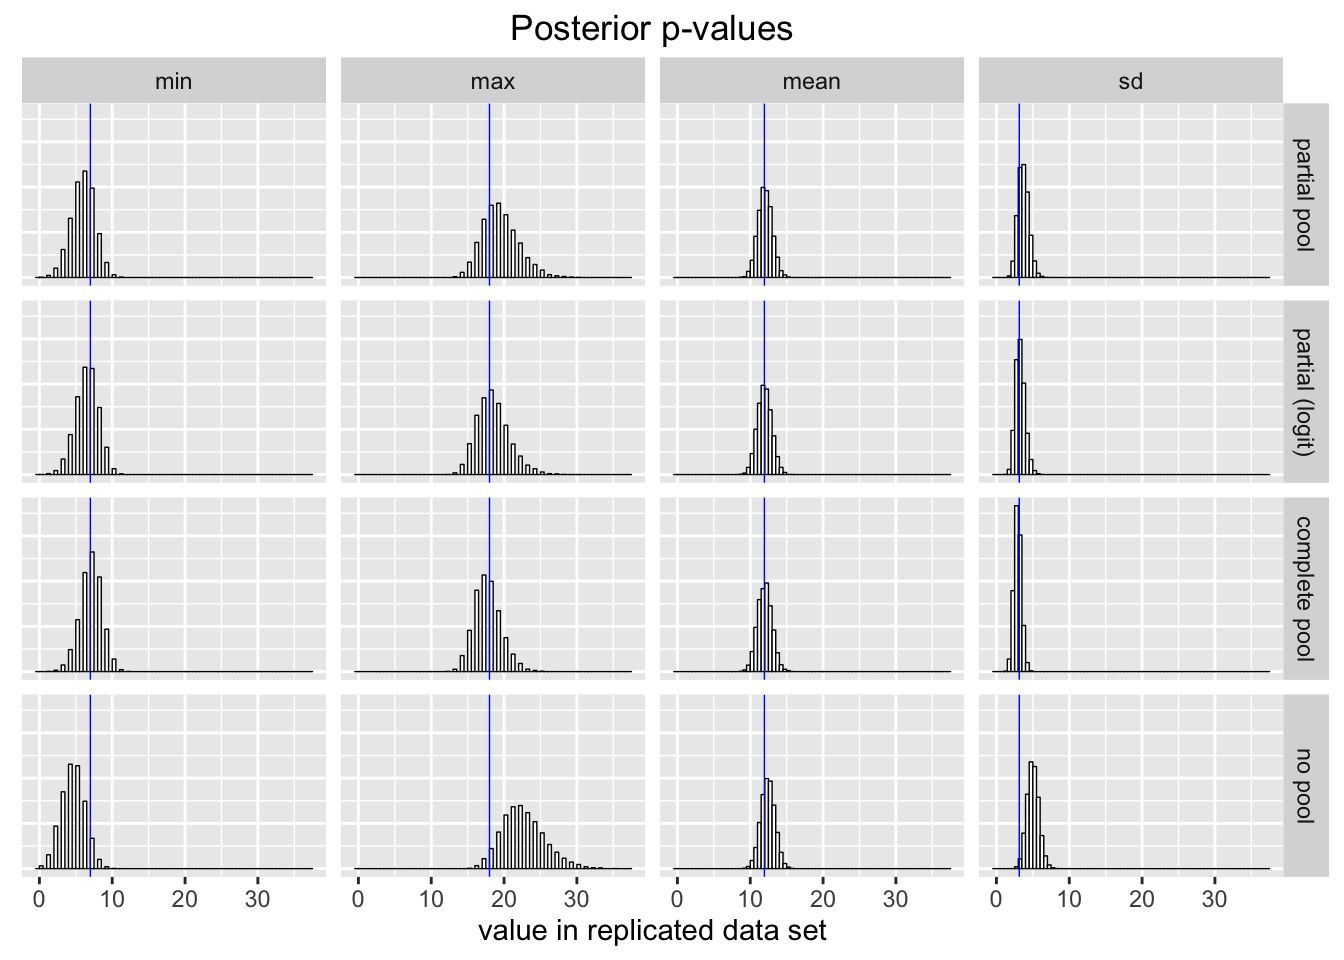
\includegraphics[height=2in]{img/posterior-p-values.png}
\end{center}


\sld{Calibration and Sharpness}
%
\begin{itemize}
\item \myemph{Calibration}:  A model is calibrated if the 50\% intervals
  contain roughly 50\% of the true intervals
\begin{subitemize}
\item technically, we expect $\mbox{Binomial}(N, 0.5)$ of $N$
  parameters to fall in their 50\% intervals
\item we can evaluate with held-out data using cross-validation
\end{subitemize}
%
\item \myemph{Sharpness}: One posterior is sharper than another if it
  concentrates more posterior mass around the true value
\begin{subitemize}
\item e.g., central posterior intervals of interest are narrower
\vfill
\item \footnotesize{see: Gneiting, Balabdaoui, and Raftery (2007) Probabilistic
    forecasts, calibration and sharpness. {\slshape JRSS B}.}
\end{subitemize}
\end{itemize}


\sld{More in the Case Study}
%
\begin{itemize}
%
\item This talk roughly followed my Stan case study:
\begin{subitemize}
\item Hierarchical Partial Pooling for Repeated Binary Trials
\end{subitemize}
%
\item Available under case studies at
\begin{subitemize}
\item \url{http://mc-stan.org/documentation}.
\end{subitemize}
%
\item Contribute case studies in knitr or Jupyter
\begin{subitemize}
\item Chris Fonnesbeck (of PyMC3 fame) wrote a great PyStan case study
  on hierarchical modeling for continuous data as a Python Jupyter
  notebook (follow above link)
\item Many more case studies, including new ones by Michael Betancourt
  on core Stan computational issues
\end{subitemize}
\end{itemize}



\mypart{}{Maximum Likelihood \\[8pt]\spc Estimation}


\sld{Observations, Counterfactuals,\\[6pt] \spc{}and Random Variables}
%
\begin{itemize}
\item Assume we observe data $y = y_1, \ldots, y_N$
\item Statistical modeling assumes even though $y$ is observed,
the values could have been different
\item John Stuart Mill first characterized this {\bfseries counterfactual} nature of statistical modeling in:
\\[3pt] {\slshape A System of Logic, Ratiocinative and Inductive} (1843)
\item In measure-theoretic language, $y$ is a {\bfseries random variable}
\end{itemize}


\sld{Likelihood Functions}
%
\begin{itemize}
\item A \myemph{likelihood function} is a probability function (density, mass, or mixed)
\[
p(y|\theta,x),
\]
where
\begin{subitemize}
\item $\theta$ is a vector of \myemph{parameters},
\item $x$ is some fixed \myemph{unmodeled data} (e.g., regression predictors or
  ``features''),
\item $y$ is some fixed \myemph{modeled data} (e.g., observations)
\end{subitemize}
\item considered as a function $\mathcal{L}(\theta)$ of $\theta$ for fixed $x$ and $y$.
\end{itemize}


\sld{Maximum Likelihood Estimation}
%
\begin{itemize}
\item \myemph{Estimate} parameters $\theta$ given observations $y$.
\item Maximum likelihood estimation (MLE) chooses
estimate that maximizes the likelihood function, i.e.,
\[
\theta^*
\ = \ \argmax_{\theta} \ \mathcal{L}(\theta)
\ = \ \argmax_{\theta} \ p(y|\theta,x)
\]
\item This function of $\mathcal{L}$ and $y$ (and $x$) is called an \myemph{estimator}
\end{itemize}


\sld{Example of MLE}
%
\begin{itemize}
\item The frequency-based estimate
\[
\theta^{*} = \frac{1}{N} \sum_{n=1}^N y_n,
\]
is the observed rate of ``success'' (outcome 1) observations.
\item This is the MLE for the model
\[
p(y|\theta)
\ = \ \prod_{n=1}^N p(y_n|\theta)
\ = \  \prod_{n=1}^N \distro{Bernoulli}(y_n|\theta)
\]
where for $u \in \setcomp{0,1}$,
{\small
\[
\distro{Bernoulli}(u|\theta) =
\begin{cases}
\theta & \text{if } u = 1
\\
1 - \theta & \text{if } u = 0
\end{cases}
\]
}
\end{itemize}


\sld{Example of MLE {\normalsize (cont.)}}
%
\vspace*{-4pt}
\begin{itemize}
\item First modeling \emph{assumption} is that data are i.i.d.,
\[
p(y|\theta) = \prod_{n=1}^N p(y_n|\theta)
\]
\item Second modeling \emph{assumption} is form of likelihood,
\[
p(y_n|\theta) = \distro{Bernoulli}(y_n|\theta)
\]
\end{itemize}


\sld{Example of MLE {\normalsize (cont.)}}
%
\begin{itemize}
\item The frequency-based estimate is the MLE
\item First derivative is zero (indicating min or max),
\[
\mathcal{L}'_y(\theta^*) = 0,
\]
\item Second derivative is negative (indicating max),
\[
\mathcal{L}''_y(\theta^*) < 0.
\]
\end{itemize}


\sld{MLEs can be Dangerous!}
%
\begin{itemize}
\item Recall the cancer cluster example
\item Accuracy is low with small counts
\item What we need are hierarchical models (stay tuned)
\end{itemize}


\mypart{}{(Un-)Bayesian \\[8pt]\spc{}Point Estimation}


\sld{MAP Estimator}
%
\vspace*{-4pt}
\begin{itemize}
\item For a Bayesian model $p(y,\theta) = p(y|\theta) \, p(\theta)$,
the max a posteriori (MAP) estimate maximizes the posterior,
\begin{eqnarray*}
\theta^{*}
& = & \argmax_{\theta} \ p(\theta|y)
\\[3pt]
& = & \argmax_{\theta} \ \frac{\displaystyle p(y|\theta) p(\theta)}{p(y)}
\\[3pt]
& = & \argmax_{\theta} \ p(y|\theta) p(\theta).
\\[3pt]
& = & \argmax_{\theta} \ \log p(y|\theta) + \log p(\theta).
\end{eqnarray*}
\item \emph{not} Bayesian because it doesn't integrate over uncertainty
\item \emph{not} frequentist because of distributions over parameters
\end{itemize}


\sld{MAP and the MLE}
%
\begin{itemize}
\item MAP estimate reduces to the MLE if the prior is uniform, i.e.,
\[
p(\theta) = c
\]
because
\begin{eqnarray*}
\theta^{*} & = & \argmax_{\theta} \ p(y|\theta) \, p(\theta)
\\[4pt]
& = & \argmax_{\theta} \ p(y|\theta) \, c
\\[4pt]
& = & \argmax_{\theta} \ p(y|\theta).
\end{eqnarray*}
\end{itemize}


\sld{Penalized Maximum Likelihood}
%
\begin{itemize}
\item The MAP estimate can be made palatable to frequentists
via philosophical sleight of hand
\item Treat the negative log prior $-\log p(\theta)$ as a ``penalty''
\item e.g., a $\distro{Normal}(\theta|\mu,\sigma)$ prior becomes a penalty function
\[
\lambda_{\theta, \mu,\sigma}
\  = \
-\left(
   \log \sigma + \frac{1}{2}\left(\frac{\theta -  \mu}{\sigma}\right)^2
 \right)
\]
\item Maximize sum of log likelihood and negative penalty
\begin{eqnarray*}
\theta^{*}
& = & \argmax_{\theta} \ \log p(y|\theta,x) - \lambda_{\theta,\mu,\sigma}
\\[4pt]
& = & \argmax_{\theta} \ \log p(y|\theta,x) + \log p(\theta|\mu,\sigma)
\end{eqnarray*}
\end{itemize}


\sld{Bayesian Point Estimates}
%
\begin{itemize}
\item Choose estimate to minimize some loss function
\item To minimize expected squared error (i.e., L2 loss), use
$\expectation{(\theta - \theta')^2 \, | \, y}$, use the posterior mean
\[
\hat{\theta}
\ = \ \argmin_{\theta'} \expectation{(\theta - \theta')^2 \, | \, y}
\ = \ \int_{\Theta} \theta \times p(\theta|y) \, d\theta.
\]
\item To minimize expected absolute error (L1 loss), $\expectation{|\theta -
    \theta'|}$, use the posterior median.
\item Other loss (utility) functions possible, the study of which falls under
  decision theory
\item All share property of involving full Bayesian inference.
\end{itemize}


\sld{Bayesian Point Estimates}
%
\begin{itemize}
\item \myemph{Posterior Mean Estimate} (min expected square error)
\[
\hat{\theta}
\ = \
\mathbb{E}\left[\theta \, | \, y \right]
\ = \
\int_{\Theta} \theta \, p(\theta \, | \, y) \, \mathrm{d}\theta
\ \approx \
\frac{1}{M} \sum_{m=1}^M \theta^{(m)}.
\]
%
\item \myemph{Posterior Median Estimate} (min expected absolute error)
\[
\bar{\theta} \ \mbox{solves} \ \mbox{Pr}[\theta > \bar{\theta}] = 0.5
\]
\[
\bar{\theta} \ \approx \ \mbox{median}(\{ \theta^{(1)}, \ldots
\theta^{(M)} \})
\]
\vspace*{-12pt}
\begin{subitemize}
\item other quantiles also estimated with posterior draws
\item need a lot of draws for accurate tail estimates
\end{subitemize}
\end{itemize}


\sld{Point Estimates for Inference?}
%
\begin{itemize}
\item Common in machine learning to generate a point estimate
  $\theta^*$, then use it for inference, $p(\tilde{y} | \theta^{*})$
\item This is \emph{defective} because it
\vspace*{-1pt}
\begin{center}
{\Large\bfseries Underestimates Uncertainty}
\end{center}
\item To properly estimate uncertainty, apply full Bayes
\item If not, (probabilistic) Dutch book can be made against you
\begin{subitemize}
\item i.e., if you use your strategy to bet, I can beat you
in the long run using full Bayes (de Finetti)
\end{subitemize}
\end{itemize}


\mypart{}{Philosophy of Probability}


\sld{Exchangeability}
%
\begin{itemize}
\item Roughly, an exchangeable probability function is such that for
a sequence of random variables $y = y_1,\ldots,y_N$,
\[
p(y) = p(\pi(y))
\]
for every $N$-permutation $\pi$ (i.e, a one-to-one mapping of $\setcomp{1,\ldots,N}$)
\item i.i.d. implies exchangeability, but not vice-versa
\end{itemize}


\sld{Exchangeability Assumptions}
%
\begin{itemize}
\item Models almost always make some kind of exchangeability assumption
\item Typically when other knowledge is not available
\begin{subitemize}
\item e.g., treat voters as conditionally i.i.d. given their age,
sex, income, education level, religous affiliation,
and state of residence
\item But voters have many more properties (hair color, height, profession, employment status, marital status, car ownership, gun ownership, etc.)
\item Missing predictors introduce additional error (on top of measurement error)
\end{subitemize}
\end{itemize}


\sld{de Finetti's Theorem}
%
\begin{itemize}
\item Given some background variables, every exchangeable sequence is conditionally i.i.d.
\item So if our i.i.d. assumptions are invalid,
\\ condition on more predictors
\end{itemize}


\sld{Bayesian vs.\ Frequentist}
%
\begin{itemize}
\item \emph{Everyone}: Model data $y$ as ``random''
\item \emph{Everyone}: Parameters have single, true (but unknown) value
\item \emph{Everyone}: Admit Bayes's rule of probability
\item \emph{Bayesians Only}: Model parameters $\theta$ as ``random''
\item \emph{Frequentists Only}: Probabilities are long-run frequencies of observables, which excludes parameters (unobservable)
\item \emph{Bayesians Only}: Allow probabilities conditioned on parameters
\end{itemize}


\sld{Random Parameters:\\[8pt]\spc{}\!Doxastic or Epistemic?}
%
\begin{itemize}
\item Bayesians treat distributions over parameters as epistemic \\
(i.e., about knowledge)
\item They do \emph{not} \ treat them as being doxastic \\
(i.e., about beliefs)
\item Priors encode our knowledge before seeing the data
\item Posteriors encode our knowledge after seeing the data
\item Bayes's rule provides the way to update our knowledge
\item People like to pretend models are ontological \\
(i.e., about what exists)
\end{itemize}

\sld{Arbitrariness:\\[8pt]\spc{}\!Priors vs.\ Likelihood}
%
\begin{itemize}
\item Bayesian analyses often criticized as subjective (arbitrary)
\item Choosing priors is no more arbitrary than choosing a likelihood
  function (or an exchangeability/i.i.d.\ assumption)
\item As George Box famously wrote (1987),
\begin{center}
\large
{\bfseries All models are wrong, but some are useful.}
\end{center}
\item This is true for frequentists as well as Bayesians
\end{itemize}


\mypart{}{What is Stan?}


\sld{What is Stan?}
%
\begin{itemize}
\item Stan is an \myemph{imperative} probabilistic programming language
\vspace*{-12pt}
  \begin{subitemize}
  \item  cf., BUGS: declarative; \ Church: functional; \ Figaro: object-oriented
  \end{subitemize}
\item Stan \myemph{program}
  \begin{subitemize}
  \item declares data and (constrained) parameter variables
  \item defines log posterior (or penalized likelihood)
  \end{subitemize}
\item Stan \myemph{inference}
  \begin{subitemize}
  \item MCMC for full Bayesian inference
  \item VB for approximate Bayesian inference
  \item MLE for penalized maximum likelihood estimation
  \end{subitemize}
\end{itemize}


\sld{Platforms and Interfaces}
%
\vspace*{-2pt}
\begin{itemize}
\item \myemph{Platforms}:  Linux, Mac OS X, Windows
\item \myemph{C++ API}: {\small portable, standards compliant (C++11)}
\item \myemph{Interfaces}
\begin{subitemize}\footnotesize
  \item \myemph{CmdStan}: Command-line or shell interface (direct executable)
  \item \myemph{RStan}: R interface (Rcpp in memory)
  \item \myemph{PyStan}: Python interface (Cython in memory)
  \item \myemph{MatlabStan}: MATLAB interface (external process)
  \item \myemph{Stan.jl}: Julia interface (external process)
  \item \myemph{StataStan}: Stata interface (external process)
  \item \myemph{MathematicaStan}: Stata interface (external process)
\end{subitemize}
\end{itemize}


\sld{Higher-Level Interfaces}
%
\begin{itemize}
\item \myemph{R Interfaces}
\begin{subitemize}
 \item \myemph{RStanArm}: regression modeling with R expressions
 \item \myemph{ShinyStan}: web-based posterior visualization, exploration
 \item \myemph{Loo}:  approximate leave-one-out cross-validation
\end{subitemize}
\item \myemph{Jupyter Containers}
\begin{subitemize}
\item \myemph{Docker} versions for R, Python, Julia
\item \myemph{SageMath}: free online server (R)
\end{subitemize}
\item From others
\begin{subitemize}
\item \myemph{Prohet} (Facebook): time-series analysis (R and Python)
\item \myemph{brms} (B\"urkner): regression modeling with R expressions
\item \myemph{rethinking} (McElreath): simplified Stan embedded in R
\end{subitemize}
\end{itemize}
\vfill


\sld{Who's Using Stan?}
%
\begin{itemize}
\item 2500+ \myemph{users group} registrations;  20,000+ \myemph{downloads}
  \small{(per version just in Rstudio)}; 1000+ Google scholar citations
\item \myemph{Biological sciences}: {\footnotesize
clinical drug trials, entomology, pharmacology, toxicology, botany,
neurology, genomics, agriculture, botany, fisheries, genomics, cellular
biology, epidemiology, population ecology, neurology
}
\item \myemph{Physical sciences}: {\footnotesize
astrophysics, particle physics, molecular biology, oceanography, climatology, biogeochemistry, materials science
}
\item \myemph{Social sciences}: {\footnotesize
 econometrics (macro and micro), population dynamics, cognitive
 science, psycholinguistics, social networks, political science,
 survey sampling
}
\item \myemph{Other}: {\footnotesize materials engineering, finance,
    actuarial science, sports, public health, recommender systems,
    educational testing, fleet maintenance, sports}
\end{itemize}


\sld{Documentation}
%
\begin{itemize}
\item {\slshape Stan User's Guide and Reference Manual}
\begin{subitemize}
\item 600+ pages
\item example models, modeling and programming advice
\item introduction to Bayesian and frequentist statistics
\item complete language specification and execution guide
\item descriptions of algorithms (NUTS, R-hat, n\_eff)
\item guide to built-in distributions and functions
\end{subitemize}
\item Installation and getting started manuals by interface
\begin{subitemize}
\item RStan, PyStan, CmdStan, MatlabStan, Stan.jl, StataStan, MathematicaStan
\end{subitemize}
\item Many written and video tutorials by users and developers
\end{itemize}


\sld{Model Sets Translated to Stan}
%
\begin{itemize}
\item BUGS examples (most of all 3 volumes)
\item Gelman and Hill (2009) {\slshape Data Analysis Using Regression and
    Multilevel/Hierarchical Models}.
\item Wagenmakers and Lee (2014) {\slshape Bayesian Cognitive
    Modeling}.
\item K\'ery and Schaub (2014) {\slshape Bayesian Population Analysis
    Using WinBUGS}.
\item Kruschke (2014) {\slshape Doing Bayesian Data Analysis}.
\end{itemize}


\sld{Books about Stan}
%
\begin{subitemize}
\footnotesize
\item Gelman and Hill (2018) {\slshape Regression and Other Stories}. Cambridge.
\item Hilbe, de Souza, and Ishida (2017) {\slshape Bayesian Models for Astrophysical Data Using R, JAGS, Python, and Stan}. Cambridge.
\item Matsuura (2016) {\slshape Bayesian Statistical Modeling Using Stan and R}. Kyoritsu. (Japanese)
\item Faraway (2016) {\slshape Extending the Linear Model with R: Generalized Linear, Mixed Effects and Nonparametric Regression Models}, 2nd Edition. CRC.
\item McElreath (2016) {\slshape Statistical Rethinking: A Bayesian course
    with R and Stan}. CRC.
\item Korner-Nievergelt et al. (2015) {\slshape Bayesian Data Analysis in
    Ecology Using Linear Models with R, BUGS, and Stan}. Academic Press.
\item Kruschke (2014) {\slshape Doing Bayesian Data Analysis, Second
    Edition: A Tutorial with R, JAGS, and Stan}. Academic Press.
\item Gelman et al. (2013) {\slshape Bayesian Data Analysis}, 3rd Edition. CRC.
\end{subitemize}


\sld{Scaling and Evaluation}
%
\begin{center}
\vspace*{-6pt}
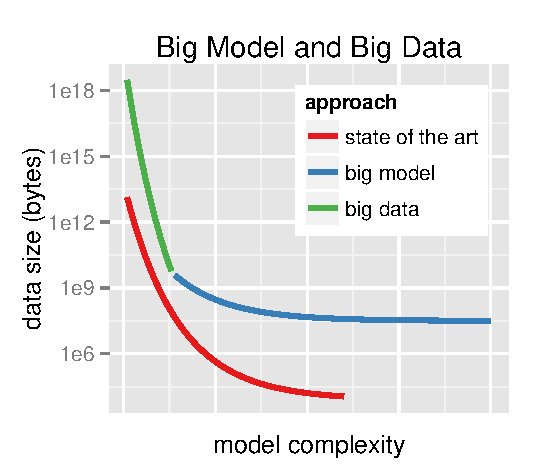
\includegraphics[width=0.4\textwidth]{img/big-model-big-data.pdf}
\vspace*{-6pt}
\end{center}
\begin{itemize}
\item Types of Scaling: data, parameters, \myemph{models}
\item Time to converge and per effective sample size: \\[2pt]
\mbox{ } \ \ \ {0.5--{\large$\infty$} times faster than BUGS \& JAGS}
\item Memory usage: \ {1--10\% of BUGS \& JAGS}
\end{itemize}


\sld{NUTS vs.\ Gibbs and Metropolis}
%
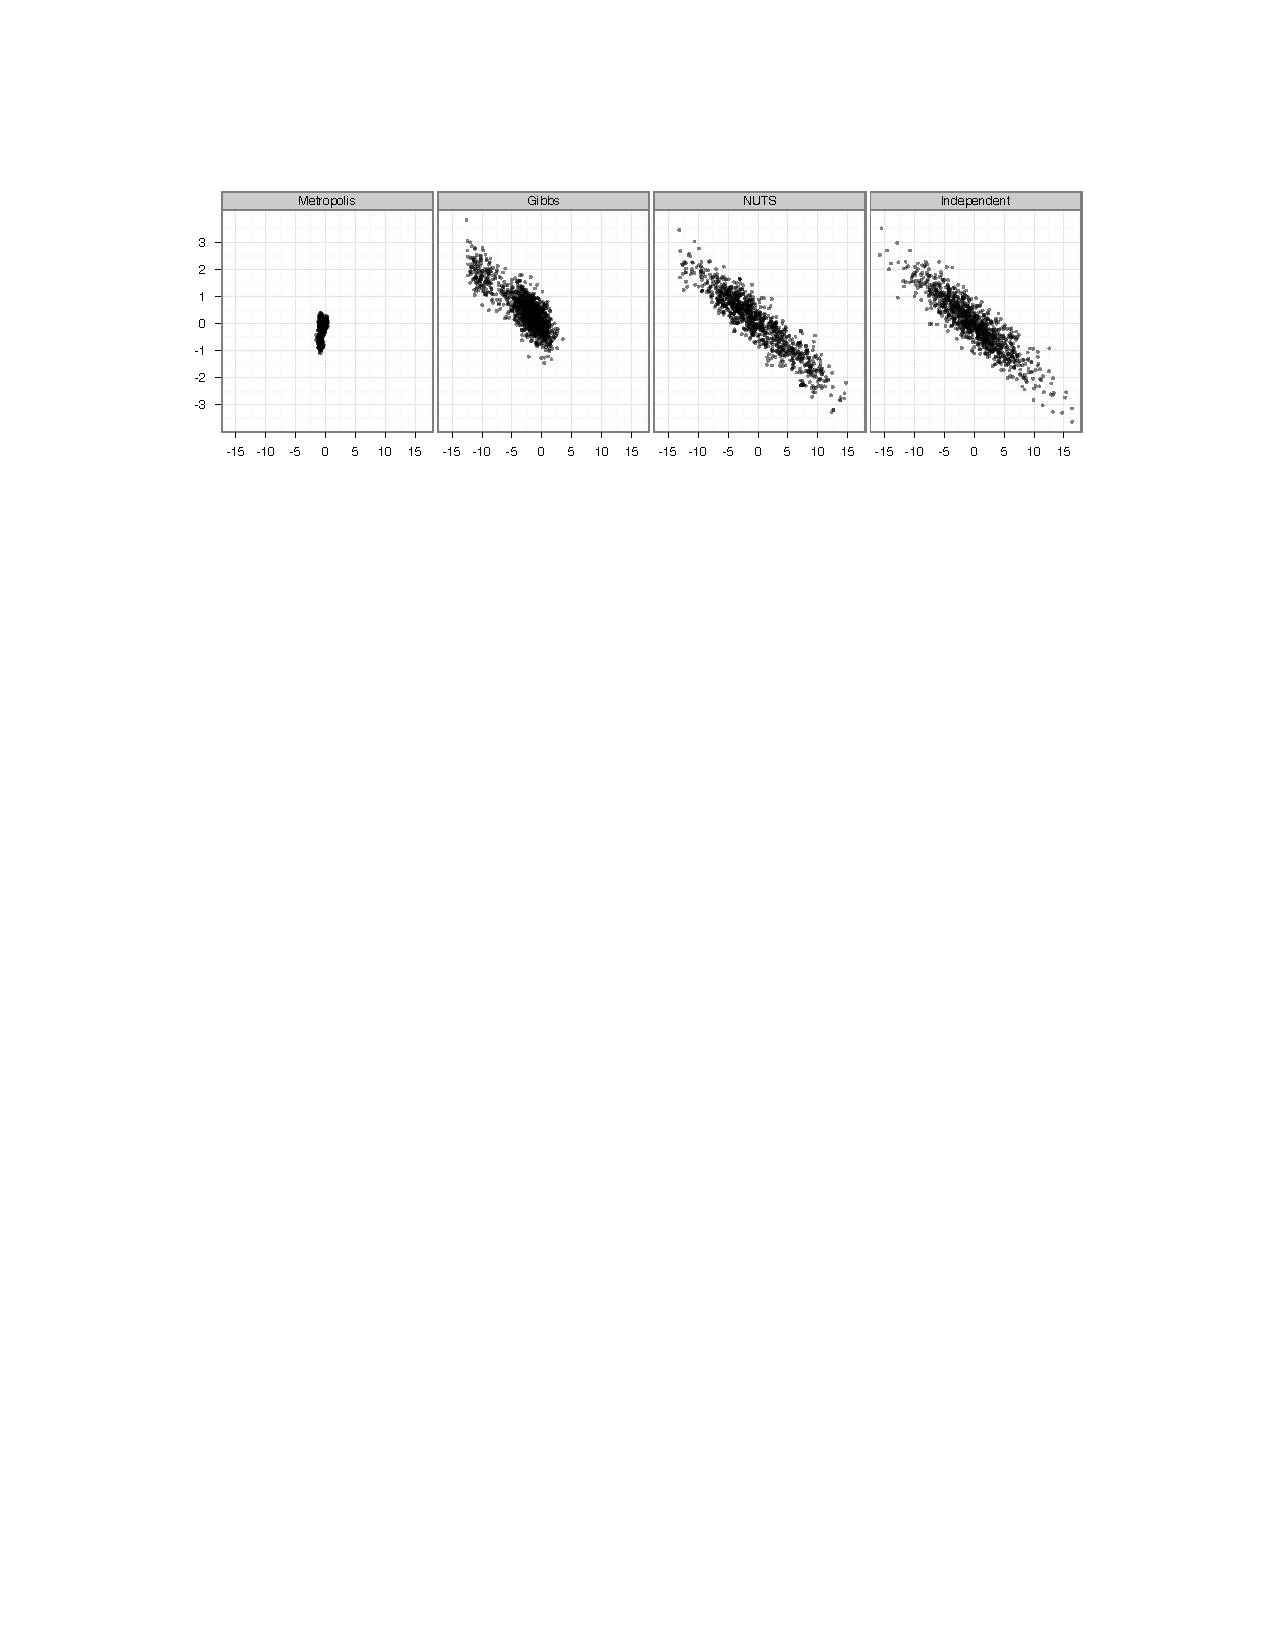
\includegraphics[width=0.9\textwidth]{img/nuts-vs.pdf}
\begin{subitemize}
\item Two dimensions of highly correlated 250-dim normal
\item \myemph{1,000,000 draws} from Metropolis and Gibbs (thin to 1000)
\item \myemph{1000 draws} from NUTS; 1000 independent draws
\end{subitemize}


\sld{Stan's Autodiff vs.\ Alternatives}

\begin{subitemize}
\item Among \myemph{C++ open-source} offerings:
Stan is \myemph{fastest} (for gradients),
\myemph{most general} (functions supported),
and \myemph{most easily extensible} (simple OO)
\end{subitemize}
\vspace*{-8pt}
\hfill
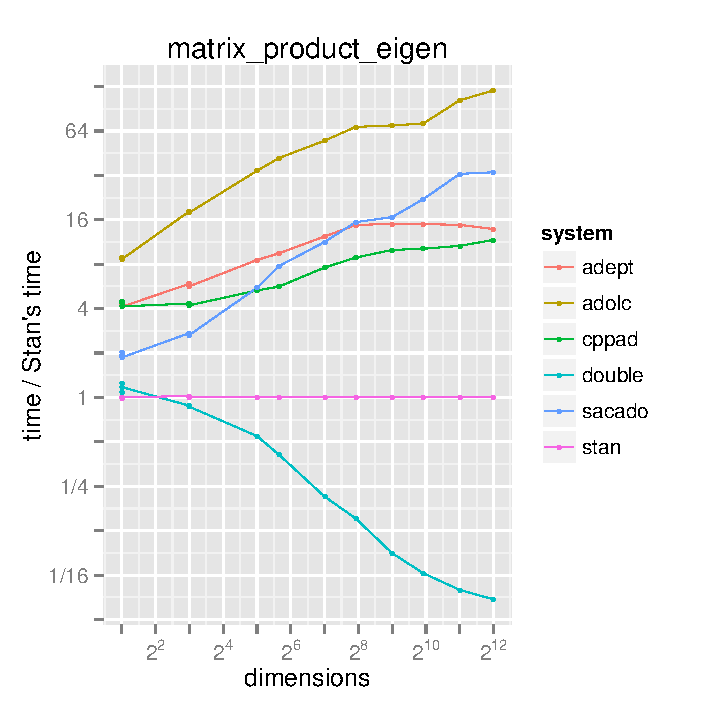
\includegraphics[width=0.45\textwidth]{img/autodiff-eval-matrix-product-eigen.pdf}
\hfill
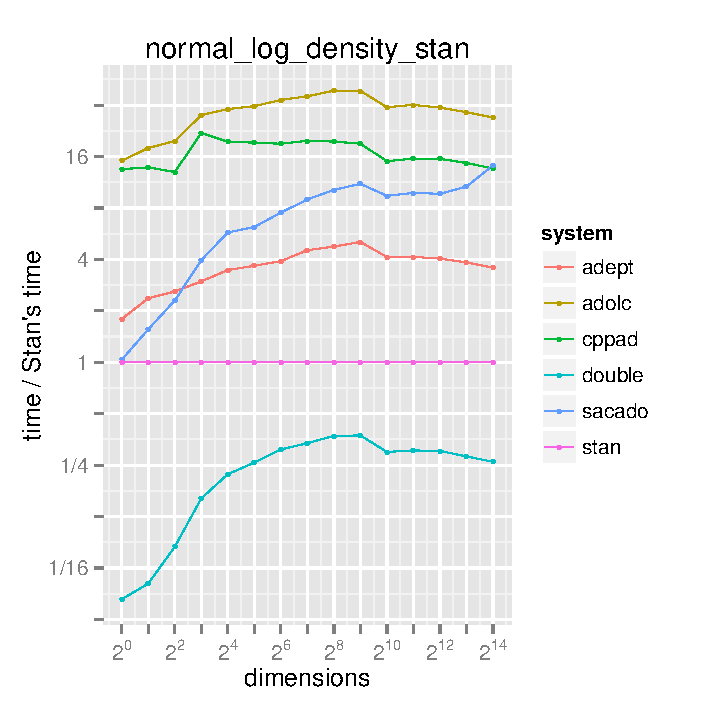
\includegraphics[width=0.45\textwidth]{img/autodiff-eval-normal-density.pdf}
\hfill



\mypart{}{Stan Language}


\sld{Stan is a Programming Language}
%
\begin{itemize}
\item \myemph{Not} a graphical specification language like BUGS or JAGS
\item Stan is a Turing-complete imperative programming langauge for specifying differentiable log densities
\begin{subitemize}
\item reassignable local variables and scoping
\item full conditionals and loops
\item functions (including recursion)
\end{subitemize}
\item With automatic ``black-box'' inference on top (though even that is tunable)
\item Programs computing same thing may have different efficiency
\end{itemize}


\sld{Basic Program Blocks}
%
\begin{itemize}
\item \myemph{\tt\bfseries data} \ (once)
  \vspace*{-4pt}
  \begin{itemize}\small
  \item {\slshape content}: declare data types, sizes, and constraints
  \item {\slshape execute}: read from data source, validate constraints
  \end{itemize}
  %
\item \myemph{\tt\bfseries parameters} \ (every log prob eval)
  \vspace*{-4pt}
  \begin{itemize}\small
  \item {\slshape content}: declare parameter types, sizes, and constraints
  \item {\slshape execute}: transform to constrained, Jacobian
  \end{itemize}
  %
\item \myemph{\tt\bfseries model} \ (every log prob eval)
  \vspace*{-4pt}
  \begin{itemize}\small
  \item {\slshape content}: statements definining posterior density
  \item {\slshape execute}: execute statements
  \end{itemize}
\end{itemize}


\sld{Derived Variable Blocks}
%
\begin{itemize}
\item \myemph{\tt\bfseries transformed data} (once after data)
  \vspace*{-4pt}
  \begin{itemize}\small
  \item {\slshape content}: declare and define transformed data variables
  \item {\slshape execute}: execute definition statements, validate constraints
  \end{itemize}
  %
\item \myemph{\tt\bfseries transformed parameters} (every log prob eval)
  \vspace*{-4pt}
  \begin{itemize}\small
  \item {\slshape content}: declare and define transformed parameter vars
  \item {\slshape execute}: execute definition statements, validate constraints
  \end{itemize}
  %
\item \myemph{\tt\bfseries generated quantities} (once per draw,
  \code{double} type)
  \vspace*{-4pt}
  \begin{itemize}\small
  \item {\slshape content}: declare and define generated quantity
    variables; \\
    includes pseudo-random number generators
    \\
    {\footnotesize (for posterior predictions, event probabilities,
      decision making)}
  \item {\slshape execute}: execute definition statements, validate constraints
  \end{itemize}
  %
\end{itemize}


\sld{Model: Read and Transform Data}
%
\begin{itemize}
\item Only done once for optimization or sampling (per chain)
\item Read data
\begin{subitemize}
\item read data variables from memory or file stream
\item validate data
\end{subitemize}
\item Generate transformed data
\begin{subitemize}
\item execute transformed data statements
\item validate variable constraints when done
\end{subitemize}
\end{itemize}


\sld{Model: Log Density}
%
\begin{itemize}
\item \emph{Given} parameter values on unconstrained scale
\item Builds expression graph for log density (start at 0)
\item Inverse transform parameters to constrained scale
\begin{subitemize}
\item constraints involve non-linear transforms
\item e.g.,  positive constrained $x$ to unconstrained $y = \log x$
\end{subitemize}
\item account for curvature in change of variables
\begin{subitemize}
\item e.g., unconstrained $y$ to positive $x = \log^{-1}(y) =
  \exp(y)$
\item e.g., add log Jacobian determinant, $\log |\frac{d}{dy} \exp(y)| = y$
\end{subitemize}
\item Execute model block statements to increment log density
\end{itemize}

\sld{Model: Log Density Gradient}
%
\begin{itemize}
\item Log density evaluation builds up expression graph
\begin{subitemize}
\item templated overloads of functions and operators
\item efficient arena-based memory management
\end{subitemize}
\item Compute gradient in backward pass on expression graph
\begin{subitemize}
\item propagate partial derivatives via chain rule
\item work backwards from final log density to parameters
\item dynamic programming for shared subexpressions
\end{subitemize}
\item Linear multiple of time to evalue log density
\end{itemize}


\sld{Model: Generated Quantities}
%
\begin{itemize}
\item \myemph{Given} parameter values
\item Once per iteration (not once per leapfrog step)
\item May involve (pseudo) random-number generation
\begin{subitemize}
\item Executed generated quantity statements
\item Validate values satisfy constraints
\end{subitemize}
\item Typically used for
\begin{subitemize}
\item Event probability estimation
\item Predictive posterior estimation
\end{subitemize}
\item Efficient because evaluated with \code{double} types (no autodiff)
\end{itemize}


\sld{Variable Transforms}
%
\begin{itemize}
\item Code HMC and optimization with $\mathbb{R}^n$ \myemph{support}
\item Transform constrained parameters to unconstrained
  \vspace*{-2pt}
  {\small
    \begin{itemize}
    \item lower (upper) bound: offset (negated) log transform
    \item lower and upper bound: scaled, offset logit transform
    \item simplex: centered, stick-breaking logit transform
    \item ordered: free first element, log transform offsets
    \item unit length: spherical coordinates
    \item covariance matrix: Cholesky factor positive diagonal
    \item correlation matrix: rows unit length via quadratic stick-breaking
    \end{itemize}
  }
\end{itemize}


\sld{Variable Transforms (cont.)}
%
\begin{itemize}
\item Inverse transform from unconstrained $\mathbb{R}^n$
\item Evaluate log probability in model block on natural scale
\item Optionally adjust log probability for change of variables
\begin{subitemize}
\item adjustment for MCMC and variational, not MLE
\item add log determinant of inverse transform Jacobian
\item automatically differentiable
\end{subitemize}
\end{itemize}


\sld{Variable and Expression Types}
%
\\[3pt]
\hspace*{17pt}Variables and expressions are \myemph{strongly, statically typed}.
\begin{itemize}
\item \myemph{Primitive}: {\tt\small int}, \ {\tt\small real}
\item \myemph{Matrix}: {\tt\small matrix[M,N]}, \ {\tt\small vector[M]}, \ {\tt\small row\_vector[N]}
\item \myemph{Bounded}: primitive or matrix, with
  \\ {\tt\small <lower=L>}, \ {\tt\small <upper=U>}, \ {\tt\small <lower=L,upper=U>}
\item \myemph{Constrained Vectors}: {\tt\small simplex[K]}, \ {\tt\small
    ordered[N]},
  \\ {\tt\small positive\_ordered[N]}, \ {\tt\small unit\_length[N]}
\item \myemph{Constrained Matrices}: {\tt\small cov\_matrix[K]}, \ {\tt\small
    corr\_matrix[K]}, \ {\tt\small cholesky\_factor\_cov[M,N]}, \
  {\tt\small cholesky\_factor\_corr[K]}
\item \myemph{Arrays:}  of any type (and dimensionality)
\end{itemize}


\sld{Integers vs.\ Reals}
%
\begin{itemize}
\item Different types (conflated in BUGS, JAGS, and R)
\item Distributions and assignments care
\item Integers may be assigned to reals but not vice-versa
\item Reals have not-a-number, and positive and negative infinity
\item Integers single-precision up to +/- 2 billion
\item Integer division rounds (Stan provides warning)
\item Real arithmetic is inexact and reals should not be (usually) compared with \code{==}
\end{itemize}


\sld{Arrays vs. Vectors \& Matrices}
%
\begin{itemize}
\item Stan separates arrays, matrices, vectors, row vectors
\item Which to use?
\item Arrays allow most efficient access (no copying)
\item Arrays stored first-index major (i.e., 2D are row major)
\item Vectors and matrices required for matrix and linear algebra functions
\item Matrices stored column-major
\item Are not assignable to each other, but there are conversion functions
\end{itemize}


\sld{Logical Operators}
%
\vfill
\noindent\spc
{\footnotesize
  \begin{tabular}{c|ccl|l}
    {\it Op.} & {\it Prec.} & {\it Assoc.} & {\it
      Placement} & {\it Description}
    \\ \hline \hline
    \code{||} & 9 & left & binary infix & logical or
    \\ \hline
    \Verb|&&| & 8 & left & binary infix & logical and
    \\ \hline
    \Verb|==| & 7 & left & binary infix & equality
    \\
    \Verb|!=| & 7 & left & binary infix & inequality
    \\ \hline
    \Verb|<| & 6 & left & binary infix & less than
    \\
    \Verb|<=| & 6 & left & binary infix & less than or equal
    \\
    \Verb|>| & 6 & left & binary infix & greater than
    \\
    \Verb|>=| & 6 & left & binary infix & greater than or equal
  \end{tabular}
}
\vfill
\vfill


\sld{Arithmetic and Matrix Operators}
%
\vfill
\noindent\spc
{\footnotesize
  \begin{tabular}{c|ccl|l}
    {\it Op.} & {\it Prec.} & {\it Assoc.} & {\it
      Placement} & {\it Description}
    \\ \hline \hline

    \code{+} & 5 & left & binary infix & addition
    \\
    \code{-} & 5 & left & binary infix & subtraction
    \\ \hline
    \code{*} & 4 & left & binary infix & multiplication
    \\
    \code{/} & 4 & left & binary infix & (right) division
    \\ \hline
    \Verb|\| & 3 & left & binary infix & left division
    \\ \hline
    \code{.*} & 2 & left & binary infix & elementwise multiplication
    \\
    \code{./} & 2 & left & binary infix & elementwise division
    \\ \hline
    \code{!} & 1 & n/a & unary prefix & logical negation
    \\
    \code{-} & 1 & n/a & unary prefix & negation
    \\
    \code{+} & 1 & n/a & unary prefix & promotion (no-op in Stan)
    \\ \hline
    \Verb|^| & 2 & right & binary infix & exponentiation
    \\ \hline
    \code{'} & 0 & n/a & unary postfix & transposition
    \\ \hline \hline
    \code{()} & 0 & n/a & prefix, wrap & function application
    \\
    \code{[]} & 0 & left & prefix, wrap & array, matrix indexing
  \end{tabular}
}


\sld{Assignment Operators}
%
\vfill
\noindent\spc
{\footnotesize
  \begin{tabular}{c|ccl|l}
    {\it Op.} & {\it Description} \\ \hline \hline
    \code{=} & assignment \\
    \code{+=} & compound add and assign \\
    \code{-=} & compound subtract and assign \\
    \code{*=} & compound mulitply and assign \\
    \code{/=} & compound divide and assign \\
    \code{.*=} & compound elementwise mulitply and assign \\
    \code{./=} & compound elementwise divide and assign \\

  \end{tabular}
}
%
\begin{itemize}
\item these work with all relevant matrix types
\begin{subitemize}
\item e.g., \Verb|matrix *= matrix;|
\end{subitemize}
\end{itemize}


\sld{Built-in Math Functions}
%
\begin{itemize}
\item All built-in \myemph{C++ functions and operators}
  \\
  {\footnotesize C math, TR1, C++11, including all trig, pow, and
    special log1m, erf, erfc, fma, atan2, etc.}
\item Extensive library of \myemph{statistical functions}
  \\
  {\footnotesize e.g., softmax,
    log gamma and digamma functions, beta functions, Bessel functions of
    first and second kind, etc.}
  %
\item Efficient, arithmetically stable \myemph{compound functions}
  \\
  {\footnotesize e.g., multiply log, log sum of
    exponentials, log inverse logit}
\end{itemize}


\sld{Built-in Matrix Functions}
%
\begin{itemize}\small
\item \myemph{Basic arithmetic}: all arithmetic operators
\item \myemph{Elementwise arithmetic}: vectorized operations
\item \myemph{Solvers}: matrix division, (log) determinant,
  inverse
\item \myemph{Decompositions}: QR, Eigenvalues and Eigenvectors,
  \\
  Cholesky factorization, singular value decomposition
\item \myemph{Compound Operations}: quadratic forms, variance scaling, etc.
\item \myemph{Ordering, Slicing, Broadcasting}: sort, rank, block, rep
\item \myemph{Reductions}: sum, product, norms
\item \myemph{Specializations}: triangular, positive-definite,
\end{itemize}


\sld{Statements}
%
\vspace*{-4pt}
\begin{itemize}
\item \myemph{Sampling}: \ {\footnotesize \Verb|y ~ normal(mu,sigma)|}
  \ \ \ {\footnotesize (increments log probability)}
  %
\item \myemph{Log probability}: \ {\footnotesize increment\_log\_prob(lp);}
\item \myemph{Assignment}: \  {\footnotesize \code{y\_hat <- x * beta};}
  %
\item \myemph{For loop}: \ {\footnotesize \code{for (n in 1:N) ...}}
  %
\item \myemph{While loop}: \ {\footnotesize \code{while (cond) ...}}
  %
\item \myemph{Conditional}: \ {\footnotesize
    \code{if (cond) ...; else if (cond) ...;  else ...;}}
\item \myemph{Block}: \ {\footnotesize \Verb|{ ... }|}  \ \ \ {\footnotesize
    (allows local variables)}
\item \myemph{Print}: \ {\footnotesize \code{print("theta=",theta);}}
\item \myemph{Reject}:
\ {\footnotesize
    \code{reject("arg to foo must be positive, found y=", y);}}
\item \myemph{Break, Continue}: \ {\footnotesize \code{break}, \code{continue}}
\end{itemize}


\sld{``Sampling'' Increments Log Prob}
%
\begin{itemize}
\item A Stan program defines a log posterior
\begin{subitemize}
\item typically through log joint and Bayes's rule
\end{subitemize}
\item Sampling statements are just ``syntactic sugar''
\item A shorthand for incrementing the log posterior
\item The following define the same$^*$ posterior
\begin{itemize}
\item \Verb|y ~ poisson(lambda);|
\item \Verb|increment_log_prob(poisson_log(y, lamda));|
\end{itemize}
\item ${}^{*}$ up to a constant
\item Sampling statement drops constant terms
\end{itemize}


\sld{Local Variable Scope Blocks}
%
\begin{itemize}
\item
\begin{Verbatim}
  y ~ bernoulli(theta);
\end{Verbatim}
is more efficient with sufficient statistics
{\small
\begin{Verbatim}
  {
    real sum_y;  // local variable
    sum_y <- 0;
    for (n in 1:N)
      sum_y <- a + y[n];   // reassignment
    sum_y ~ binomial(N, theta);
  }
\end{Verbatim}
}
\item Simpler, but roughly same efficiency:
\begin{Verbatim}
    sum(y) ~ binomial(N, theta);
\end{Verbatim}
\end{itemize}


\sld{User-Defined Functions}
%
\begin{itemize}
\item \myemph{\tt\bfseries functions} \ (compiled with model)
  \vspace*{-4pt}
  \begin{itemize}\small
  \item {\slshape content}: declare and define general (recursive) functions
    \\
    {\small (use them elsewhere in program)}
  \item {\slshape execute}: compile with model
  \end{itemize}
  \vspace*{6pt}
\item Example
  \\[6pt]
  \begin{minipage}[t]{0.8\textwidth}
    \footnotesize
    \begin{Verbatim}
      functions {

        real relative_difference(real u, real v) {
          return 2 * fabs(u - v) / (fabs(u) + fabs(v));
        }

      }
    \end{Verbatim}
  \end{minipage}
\end{itemize}


\sld{Special User-Defined Functions}
%
\begin{itemize}
\item When declared with appropriate naming, user-defined functions
  may
\begin{subitemize}
\item be used in sampling statements: \code{real} return and suffix \Verb|_lpdf| or \Verb|_lpmf|
\item use RNGs: suffix \Verb|_rng|
\item use target accumulator:  suffix \Verb|_lp|
\end{subitemize}
\end{itemize}


\sld{Differential Equation Solver}
%
\begin{itemize}
\item System expressed as function
\begin{subitemize}
\item given state ($y$) time ($t$), parameters ($\theta$), and data ($x$)
\item return derivatives ($\partial y / \partial t$) of state w.r.t. time
\end{subitemize}
\item Simple harmonic oscillator diff eq
{\footnotesize
\begin{Verbatim}
    real[] sho(real t,         // time
               real[] y,       // system state
               real[] theta,   // params
               real[] x_r,     // real data
               int[] x_i) {    // int data
      real dydt[2];
      dydt[1] <- y[2];
      dydt[2] <- -y[1] - theta[1] * y[2];
      return dydt;
   }
\end{Verbatim}
}
\end{itemize}


\sld{Differential Equation Solver (cont.)}
%
\begin{itemize}
\item Solution via functional, given initial state (\code{y0}),
initial time (\code{t0}), desired solution times (\code{ts})
{\footnotesize
\begin{Verbatim}
  mu_y <- integrate_ode(sho, y0, t0, ts, theta, x_r, x_i);
\end{Verbatim}
}
\item Use noisy measurements of $y$ to estimate $\theta$
\begin{Verbatim}
y ~ normal(mu_y, sigma);
\end{Verbatim}
\begin{subitemize}
\item Pharmacokinetics/pharmacodynamics (PK/PD),
\item soil carbon respiration with biomass input and breakdown
\end{subitemize}
\end{itemize}


\sld{Built-in Diff Eq Solvers}
%
\begin{itemize}
\item \myemph{Non-stiff solver}: Runge-Kutta 4th/5th order (RK45)
\item \myemph{Stiff solver}:  backward-differentiation formula (BDF)
\begin{subitemize}
\item slower
\item more robust for derivatives of different scales or high
  curvature
\end{subitemize}
\item specified by suffix \Verb|_bdf| or \Verb|_rk45|
\end{itemize}


\sld{Diff Eq Derivatives}
%
\begin{itemize}
\item User defines system $\frac{\partial}{\partial t} y$
\item Need derivatives of solution $y$ w.r.t.\ parameters $\theta$
\item Couple derivatives of system  w.r.t. parameters
\[
\left(
\frac{\partial}{\partial t} \, y, \ \
\frac{\partial}{\partial t} \, \frac{\partial}{\partial \theta} \, y
\right)
\]
\item Calculate coupled system via nested autodiff of second term
\[
\frac{\partial}{\partial t} \, \frac{\partial}{\partial \theta} \, y
\ = \
\frac{\partial}{\partial \theta} \, \frac{\partial}{\partial t} \, y.
\]
\end{itemize}


\sld{Distribution Library}
%
\begin{itemize}
\item Each distribution has
  \vspace*{-4pt}
  \begin{itemize}\small
  \item log density or mass function
  \item cumulative distribution functions, plus complementary versions,
    plus log scale
  \item Pseudo-random number generators
  \end{itemize}
\item Alternative parameterizations
  \\
  {\footnotesize (e.g., Cholesky-based multi-normal,
    log-scale Poisson, logit-scale Bernoulli)}
\item New multivariate correlation matrix density: LKJ
  \\
  {\footnotesize degrees of freedom controls
    shrinkage to (expansion from) unit matrix}
\end{itemize}


\sld{Print and Reject}
%
\begin{itemize}
\item Print statements are for \myemph{debugging}
\begin{subitemize}
\item printed every log prob evaluation
\item print values in the middle of programs
\item check when log density becomes undefined
\item can embed in conditionals
\end{subitemize}
\item Reject statements are for \myemph{error checking}
\begin{subitemize}
\item typically function argument checks
\item cause a rejection of current state (0 density)
\end{subitemize}
\end{itemize}


\sld{Prob Function Vectorization}
%
\begin{itemize}
\item Stan's probability functions are vectorized for speed
\begin{subitemize}
\item removes repeated computations (e.g., $-\log \sigma$ in normal)
\item reduces size of expression graph for differentation
\end{subitemize}
\item Consider: \ \Verb|y ~ normal(mu, sigma);|
\item Each of \code{y}, \code{mu}, and \code{sigma} may be any of
\begin{subitemize}
\item scalars (integer or real)
\item vectors (row or column)
\item 1D arrays
\end{subitemize}
\item All dimensions must be scalars or having matching sizes
\item Scalars are broadcast (repeated)
\end{itemize}


\sld{Parsing and Compilation}
%
\begin{itemize}
\item Stan code \myemph{parsed} to abstract syntax tree (AST)
  \\ {\footnotesize (Boost Spirit Qi, recursive descent, lazy semantic
    actions)}
\item C++ model class \myemph{code generation} from AST
  \\ {\footnotesize (Boost Variant)}
\item C++ code \myemph{compilation}
\item \myemph{Dynamic linking} for RStan, PyStan
\end{itemize}




\mypart{}{What Stan Does}


\sld{Full Bayes: No-U-Turn Sampler}
%
\begin{itemize}
\item Adaptive \myemph{Hamiltonian Monte Carlo} (HMC)
\begin{subitemize}
\item \myemph{Potential Energy}: negative log posterior
\item \myemph{Kinetic Energy}: random standard normal per iteration
\end{subitemize}
  %
\item Adaptation \myemph{during warmup}
  \vspace*{-4pt}
  \begin{itemize}\small
  \item step size adapted to target total acceptance rate
  \item mass matrix (scale/rotation) estimated with regularization
  \end{itemize}
  %
\item Adaptation \myemph{during sampling}
  \begin{subitemize}
  \item simulate forward and backward in time until U-turn
    \item \myemph{slice sample} along path
  \end{subitemize}
  %
\vfill
\hfill
{\footnotesize (Hoffman and Gelman 2011, 2014)}
\end{itemize}


\sld{Posterior Inference}
%
\begin{itemize}
\item Generated quantities block for \myemph{inference}:
  \\ {\small \mbox{ } \ \ \ predictions, decisions, and event probabilities}
\item \myemph{Extractors} for samples in RStan and PyStan
\item Coda-like \myemph{posterior summary}
  \vspace*{-4pt}
  \begin{itemize}\small
  \item posterior mean w.\ MCMC std.\ error, std.\ dev., quantiles
  \item split-$\hat{R}$ multi-chain convergence diagnostic (Gelman/Rubin)
  \item multi-chain effective sample size estimation (FFT algorithm)
  \end{itemize}
\item Model comparison with \myemph{WAIC}
\begin{subitemize}
\item in-sample approximation to cross-validation
\end{subitemize}
\end{itemize}


\sld{MAP / Penalized MLE}
%
\begin{itemize}
\item Posterior \myemph{mode finding} via L-BFGS optimization
  \\ {\footnotesize (uses model gradient, efficiently approximates Hessian)}
\item \myemph{Disables Jacobians} for parameter inverse transforms
\item Models, data, initialization as in MCMC
  \vfill
  \item  \myemph{Standard errors} on unconstrained scale
    \\
    {\footnotesize  (estimated using curvature of penalized log likelihood function}
\item \myemph{Very Near Future}
  \vspace*{-4pt}
  \begin{itemize}\small
  \item Standard errors \myemph{on constrained scale})
    \\
    {\footnotesize  (sample unconstrained approximation and inverse transform)}
  \end{itemize}
\end{itemize}


\sld{``Black Box'' Variational Inference}
%
\begin{itemize}
\item \myemph{Black box} so can fit any Stan model
\item Multivariate \myemph{normal approx to unconstrained} posterior
\begin{subitemize}
\item covariance: diagonal mean-field or full rank
\item not Laplace approx --- around posterior mean, not mode
\item transformed back to constrained space (built-in Jacobians)
\end{subitemize}
\item Stochastic \myemph{gradient-descent} optimization
\begin{subitemize}
\item ELBO gradient estimated via Monte Carlo + autdiff
\end{subitemize}
\item Returns \myemph{approximate posterior} mean / covariance
\item Returns \myemph{sample} transformed to constrained space
\end{itemize}


\sld{Stan as a Research Tool}
%
\begin{itemize}
\item Stan can be used to \myemph{explore algorithms}
\item Models transformed to \myemph{unconstrained support} on $\mathbb{R}^n$
\item Once a model is compiled, have
  \vspace*{-4pt}
  \begin{itemize}\small
  \item \myemph{log probability, gradient, and Hessian}
  \item data I/O and parameter initialization
  \item model provides variable names and dimensionalities
  \item transforms to and from constrained representation
    \\ {\footnotesize (with or without Jacobian)}
  \end{itemize}
\end{itemize}



\mypart{}{Under Stan's Hood}


\sld{Euclidean Hamiltonian Monte Carlo}
%
\begin{itemize}
\item \myemph{Phase space}: $q$ position (parameters); \ $p$ momentum
\item \myemph{Posterior density}: $\pi(q)$
\item \myemph{Mass matrix}: $M$
\item \myemph{Potential energy}: $V(q) = -\log \pi(q)$
\item \myemph{Kinetic energy}: $T(p) = \frac{1}{2} p^{\top} M^{-1} p$
\item \myemph{Hamiltonian}:  $H(p,q) = V(q) + T(p)$
\item \myemph{Diff eqs}:
  \[
  \frac{dq}{dt} \ = \  + \frac{\partial H}{\partial p}
  \hspace*{48pt}
  \frac{dp}{dt} \ = \ - \frac{\partial H}{\partial q}
  \]
\end{itemize}


\sld{Leapfrog Integrator Steps}
%
\begin{itemize}
\item Solves Hamilton's equations by \myemph{simulating dynamics}
  \\
  {\footnotesize (symplectic [volume preserving]; $\epsilon^3$ error per step, $\epsilon^2$ total error)}
\item Given: \myemph{step size} $\epsilon$, \myemph{mass matrix} $M$, \myemph{parameters} $q$
\item \myemph{Initialize kinetic} energy, $p \sim {\sf
    Normal}(0,\mbox{\bf I})$
\item \myemph{Repeat} for $L$ leapfrog steps:
  \begin{eqnarray*}
    p & \leftarrow &
    p - \frac{\epsilon}{2} \, \frac{\partial V(q)}{\partial q}
    \ \ \ \ \ \ \mbox{[half step in momentum]}
    \\[6pt]
    q & \leftarrow &
    q + \epsilon \, M^{-1} \, p
    \ \ \ \ \ \ \ \  \mbox{[full step in position]}
    \\[6pt]
    p & \leftarrow &
    p - \frac{\epsilon}{2} \, \frac{\partial V(q)}{\partial q}
    \ \ \ \ \ \ \mbox{[half step in momentum]}
  \end{eqnarray*}
\end{itemize}


\sld{Reverse-Mode Auto Diff}
%
\begin{itemize}
\item Eval gradient in (usually small) multiple of function eval time
\begin{subitemize}
\item independent of dimensionality
\item time proportional to number of expressions evaluated
\end{subitemize}
%
\item Result accurate to machine precision (cf. finite diffs)
\item Function evaluation builds up \myemph{expression tree}
\item Dynamic program propagates \myemph{chain rule} in reverse pass
\item Reverse mode computes $\nabla g$ in one
  pass for a function $f : \mathbb{R}^N \rightarrow \mathbb{R}$
\end{itemize}


\sld{Autodiff Expression Graph}
%
\\
\hspace*{6pt}
\begin{minipage}{0.56\textwidth}
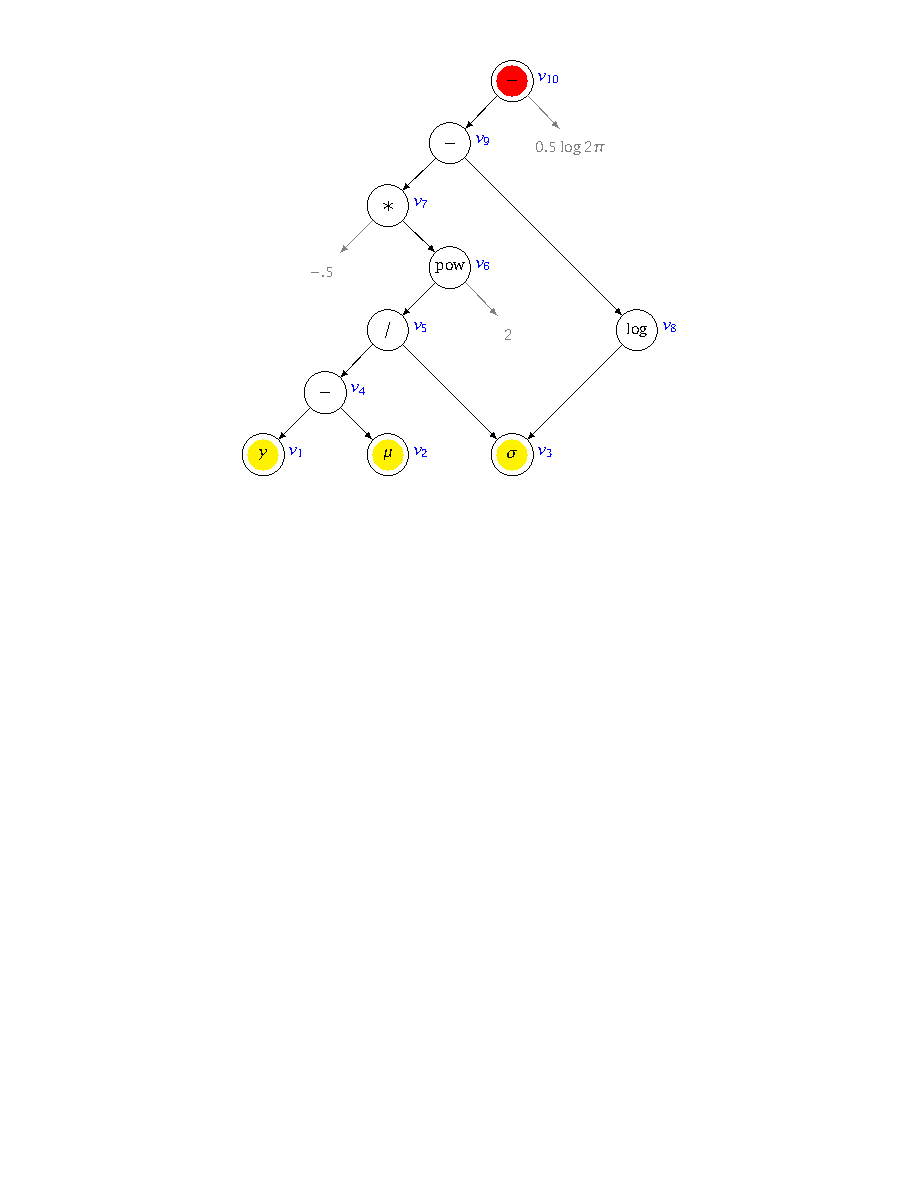
\includegraphics[width=\textwidth]{img/agrad-expression-graph.pdf}
\end{minipage}
\hspace*{-24pt}
\begin{minipage}{0.44\textwidth}
%
\footnotesize
\[
\begin{array}{l}
f(y, \mu, \sigma)
\\[4pt]
\mbox{ } \ = \ \log \left( \distro{Normal}(y|\mu,\sigma) \right)
\\[4pt]
\mbox{ } \ = \ -\frac{1}{2} \left( \frac{y - \mu}{\sigma} \right)^2
    - \log \sigma
    - \frac{1}{2} \log (2 \pi)
\end{array}
\]
\\
%
\[
\begin{array}{l}
\mbox{ } \hspace*{24pt}
\frac{\partial}{\partial y} f(y,\mu,\sigma)
\\[2pt]
\mbox{ } \hspace*{48pt} = \  -(y - \mu) \sigma^{-2}
\\[8pt]
\mbox{ } \hspace*{24pt} \frac{\partial}{\partial \mu} f(y,\mu,\sigma)
\\[2pt]
\mbox{ } \hspace*{48pt} = \ (y - \mu) \sigma^{-2}
\\[8pt]
\mbox{ } \hspace*{24pt} \frac{\partial}{\partial \sigma} f(y,\mu,\sigma)
\\[2pt]
\mbox{ } \hspace*{48pt} = \ (y - \mu)^2 \sigma^{-3} - \sigma^{-1}
\end{array}
\]
\end{minipage}


\sld{Autodiff Partials}
%
\begin{center}\footnotesize
\begin{tabular}{c||c|cc}
{\it var} & {\it value} & \multicolumn{2}{|c}{\it partials}
\\ \hline \hline
$v_1$ & $y$
\\[2pt]
$v_2$ & $\mu$
\\[2pt]
$v_3$ & $\sigma$
\\[2pt]
$v_4$ & $v_1 - v_2$ & $\partial v_4 / \partial v_1 = 1$
                   & $\partial v_4 / \partial v_2 = -1$
\\[4pt]
$v_5$ & $v_4 / v_3$ & $\partial v_5 / \partial v_4 = 1/v_3$
                    & $\partial v_5 / \partial v_3 = -v_4 v_3^{-2}$
\\[4pt]
$v_6$ & $\left(v_5\right)^2$
      & \multicolumn{2}{c}{$\partial v_6 / \partial v_5 = 2 v_5$}
\\[4pt]
$v_7$ & $(-0.5) v_6$ & \multicolumn{2}{c}{$\partial v_7 / \partial v_6
                                          = -0.5$}
\\[4pt]
$v_8$ & $\log v_3$ & \multicolumn{2}{c}{$\partial v_8 / \partial v_3 = 1/v_3$}
\\[4pt]
$v_9$ & $v_7 - v_8$ & $\partial v_9 / \partial v_7 = 1$
                    & $\partial v_9 / \partial v_8 = -1$
\\[4pt]
$v_{10}$ & $v_9 - (0.5 \log 2\pi)$
         & \multicolumn{2}{c}{$\partial v_{10} / \partial v_9 = 1$}
\end{tabular}
\end{center}

\sld{Autodiff: Reverse Pass}
%
{\small
\[
\begin{array}{rcl|l}
{\it var} & {\it operation} & {\it adjoint} & {\it result}
\\ \hline \hline
a_{1:9} & = & 0 & a_{1:9} = 0
\\
a_{10} & = & 1 & a_{10} = 1
\\ \hline
a_{9} & {+}{=} & a_{10} \times (1) & a_9 = 1
\\
a_{7} & {+}{=} & a_9 \times (1) & a_7 = 1
\\
a_{8} & {+}{=} & a_9 \times (-1) & a_8 = -1
\\
a_{3} & {+}{=} & a_8 \times (1 / v_3) & a_3 = -1 / v_3
\\
a_{6} & {+}{=} & a_7 \times (-0.5) & a_6 = -0.5
\\
a_{5} & {+}{=} & a_6 \times (2 v_5) & a_5 = -v_5
\\
a_{4} & {+}{=} & a_5 \times (1 / v_3) & a_4 = -v_5 / v_3
\\
a_{3} & {+}{=} & a_5 \times (-v_4 v_3^{-2}) & a_3 = -1 / v_3 + v_5 v_4 v_3^{-2}
\\
a_{1} & {+}{=} & a_4 \times (1) & a_1 = -v_5 / v_3
\\
a_{2} & {+}{=} & a_4 \times (-1) & a_2 = v_5 / v_3
\end{array}
\]
}


\sld{Stan's Reverse-Mode}
%
\begin{itemize}
\item Easily extensible \myemph{object-oriented} design
%
\item \myemph{Code nodes} in expression graph for primitive functions
\begin{subitemize}
\item requires \myemph{partial derivatives}
\item built-in flexible abstract base classes
\item \myemph{lazy evaluation} of chain rule saves memory
\end{subitemize}
%
\item Autodiff through templated C++ functions
\begin{subitemize}
\item templating on each argument avoids excess promotion
\end{subitemize}
%
\end{itemize}


\sld{Stan's Reverse-Mode (cont.)}
%
\begin{itemize}
\item Arena-based \myemph{memory management}
\begin{subitemize}
\item specialized C++ \code{operator~new} for reverse-mode variables
\item custom functions inherit memory management through base
\end{subitemize}
\item Nested application to support ODE solver
\end{itemize}


\sld{Stan's Autodiff vs.\ Alternatives}
%
\vspace*{-4pt}
\begin{itemize}
\item Stan is \myemph{fastest} (and uses least memory)
\begin{subitemize}
\item among open-source C++ alternatives
\end{subitemize}
\end{itemize}
\vspace*{-8pt}
\hfill \hfill
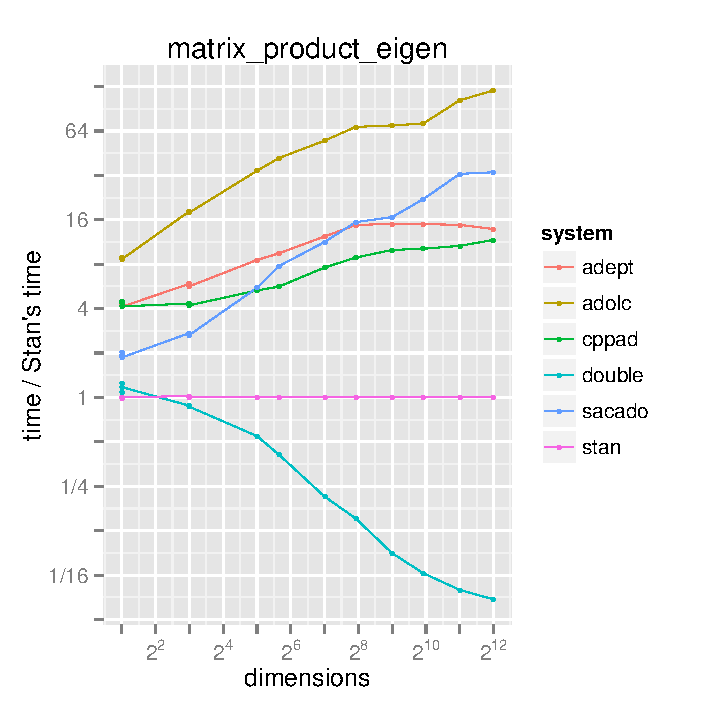
\includegraphics[width=0.48\textwidth]{img/autodiff-eval-matrix-product-eigen.pdf}
\hfill
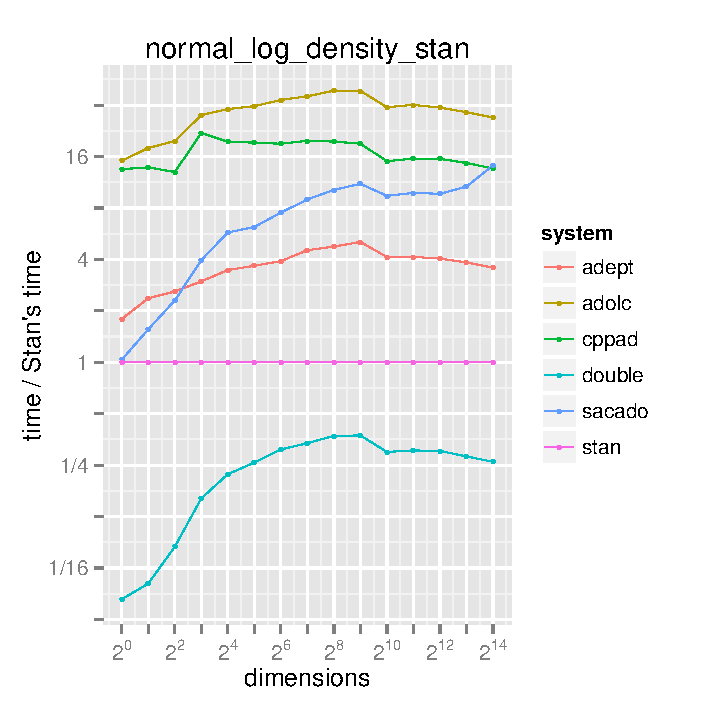
\includegraphics[width=0.48\textwidth]{img/autodiff-eval-normal-density.pdf}
\hfill \hfill


\sld{Forward-Mode Auto Diff}
%
\begin{itemize}
\item Evaluates expression graph forward from one independent variable
to any number of dependent variables
\item Function evaluation propagates \myemph{chain rule} forward
\item In one pass, computes $\frac{\partial}{\partial x} f(x)$
for a function $f : \mathbb{R} \rightarrow \mathbb{R}^N$
\begin{subitemize}
\item derivative of $N$ outputs with respect to a single input
\end{subitemize}
\end{itemize}


\sld{Stan's Forward Mode}
%
\begin{itemize}
\item Templated scalar type for value and tangent
\begin{subitemize}
\item allows higher-order derivatives
\end{subitemize}
\item Primitive functions propagate derivatives
\item No need to build expression graph in memory
\begin{subitemize}
\item much less memory intensive than reverse mode
\end{subitemize}
\item Autodiff through templated functions (as reverse mode)
\end{itemize}

\sld{Second-Order Derivatives}
%
\begin{itemize}
\item Compute Hessian (matrix of second-order partials)
\[
H_{i,j} = \frac{\partial^2}{\partial x_i \partial x_j} f(x)
\]
\item Required for Laplace covariance approximation (MLE)
\item Required for curvature (Riemannian HMC)
\item Nest reverse-mode in forward for \myemph{second order}
\item $N$ forward passes: takes gradient of derivative
\end{itemize}


\sld{Third-Order Derivatives}
%
\begin{itemize}
\item Required for Riemannian HMC
\item Graadients of Hessians (tensor of third-order partials)
\[
\frac{\partial^3}{\partial x_i \partial x_j \partial x_k} f(x)
\]
\vspace*{-12pt}
\begin{subitemize}
\item $N^2$ forward passes: gradient of derivative of derivative
\end{subitemize}
\end{itemize}


\sld{Third-order Derivatives (cont.)}
%
\begin{itemize}
\item Gradient of trace of Hessian times matrix
\begin{subitemize}
\item $\nabla \mathrm{tr}(H \, M)$, or
\item needed for Riemannian Hamiltonian Monte Carlo
\item computable in quadratic time for fixed $M$
\end{subitemize}
\end{itemize}


\sld{Jacobians}
%
\begin{itemize}
\item Assume function $f:\mathbb{R}^N \rightarrow \mathbb{R}^M$
\item Partials for multivariate function (matrix of first-order partials)
\[
J_{i,j} = \frac{\partial}{\partial x_i} f_j(x)
\]
\item Required for stiff ordinary differential equations
\begin{subitemize}
\item differentiate is coupled sensitivity autodiff for ODE system
\end{subitemize}
\item Two execution strategies
{\small
\begin{enumerate}
  \item Multiple reverse passes for rows
  \item Forward pass per column (required for stiff ODE)
\end{enumerate}
}
%
%\vfill
%
%\item Order of magnitude faster higher-order autodiff in progress
%\begin{subitemize}
%\item reuse single expression graph
%\item build-in higher-order analytic gradients
%\end{subitemize}
\end{itemize}


\sld{Autodiff Functionals}
%
\begin{itemize}
\item Functionals map templated functors to derivatives
\begin{subitemize}
\item fully encapsulates and hides all autodiff types
\end{subitemize}
\item Autodiff functionals supported
  \begin{itemize}\small
  \item gradients: $\bigoh{1}$
  \item Jacobians: $\bigoh{N}$
  \item gradient-vector product (i.e., directional derivative): $\bigoh{1}$
  \item Hessian-vector product: $\bigoh{N}$
  \item Hessian: $\bigoh{N}$
  \item gradient of trace of matrix-Hessian product: $\bigoh{N^2}$
    \\ {\footnotesize (for SoftAbs RHMC)}
  \end{itemize}
\end{itemize}


\sld{Variable Transforms}
%
\begin{itemize}
\item Code HMC and optimization with $\mathbb{R}^n$ \myemph{support}
\item Transform constrained parameters to unconstrained
  \vspace*{-2pt}
  {\small
    \begin{itemize}
    \item lower (upper) bound: offset (negated) log transform
    \item lower and upper bound: scaled, offset logit transform
    \item simplex: centered, stick-breaking logit transform
    \item ordered: free first element, log transform offsets
    \item unit length: spherical coordinates
    \item covariance matrix: Cholesky factor positive diagonal
    \item correlation matrix: rows unit length via quadratic stick-breaking
    \end{itemize}
  }
\end{itemize}


\sld{Variable Transforms (cont.)}
%
\begin{itemize}
\item Inverse transform from unconstrained $\mathbb{R}^n$
\item Evaluate log probability in model block on natural scale
\item Optionally adjust log probability for change of variables
\begin{subitemize}
\item adjustment for MCMC and variational, not MLE
\item add log determinant of inverse transform Jacobian
\item automatically differentiable
\end{subitemize}
\end{itemize}

\sld{Parsing and Compilation}
%
\begin{itemize}
\item Stan code \myemph{parsed} to abstract syntax tree (AST)
  \\ {\footnotesize (Boost Spirit Qi, recursive descent, lazy semantic
    actions)}
\item C++ model class \myemph{code generation} from AST
  \\ {\footnotesize (Boost Variant)}
\item C++ code \myemph{compilation}
\item \myemph{Dynamic linking} for RStan, PyStan
\end{itemize}


\sld{Coding Probability Functions}
%
\begin{itemize}
\item \myemph{Vectorized} to allow scalar or container arguments
  \\ {\footnotesize (containers all same shape; scalars broadcast as necessary)}
\item Avoid \myemph{repeated computations}, e.g. $\log \sigma$ in
  \hspace*{-18pt}
  {\small
    \begin{eqnarray*}
      \textstyle \log \, \mbox{\sf Normal}(y | \mu, \sigma)
      & = & \textstyle \sum_{n=1}^N \log \, \mbox{\sf Normal}(y_n | \mu,\sigma)
      \\[4pt]
      & = & \textstyle \sum_{n=1}^N  - \log \sqrt{2\pi} \ - \log \sigma \ -
      \frac{\textstyle y_n - \mu}{\textstyle 2\sigma^2}
    \end{eqnarray*}
  }
\item recursive \myemph{expression templates} to broadcast and cache scalars,
  generalize containers (arrays, matrices, vectors)
\item \myemph{traits} metaprogram to \myemph{drop constants} (e.g., $-\log
  \sqrt{2 \pi}$ or $\log \sigma$ if constant)
  and calculate intermediate and return types
\end{itemize}


\mypart{}{Stan's Autodiff}


\sld{Stan's Reverse-Mode}
%
\begin{itemize}
\item Easily extensible \myemph{object-oriented} design
\item \myemph{Code nodes} in expression graph for primitive functions
\begin{subitemize}
\item requires \myemph{partial derivatives}
\item built-in flexible abstract base classes
\item \myemph{lazy evaluation} of chain rule saves memory
\end{subitemize}
\item Autodiff through templated C++ functions
\begin{subitemize}
\item templating on each argument avoids excess promotion
\end{subitemize}
\end{itemize}


\sld{Stan's Reverse-Mode (cont.)}
%
\begin{itemize}
\item Arena-based \myemph{memory management}
\begin{subitemize}
\item specialized C++ \code{operator~new} for reverse-mode variables
\item custom functions inherit memory management through base
\end{subitemize}
\item Nested application to support ODE solver
\end{itemize}


\sld{Diff Eq Derivatives}
%
\begin{itemize}
\item Need derivatives of solution w.r.t.\ parameters
\item Couple derivatives of system  w.r.t. parameters
\[
\left(
\frac{\partial}{\partial t} \, y, \ \
\frac{\partial}{\partial t} \, \frac{\partial y}{\partial \theta}
\right)
\]
\item Calculate coupled system via \myemph{nested autodiff} of second term
\[
\frac{\partial}{\partial \theta}
\,
\frac{\partial y}{\partial t}
\]
\item Based on Eigen's Odeint package (RK45 non-stiff solver)
\end{itemize}


\sld{Stiff Diff Eqs}
%
\begin{itemize}
\item Based on CVODES implementation of BDF (Sundials)
\item CVODES builds-in efficient structure for sensitivity
\item More nested autodiff required for system Jacobian
\begin{subitemize}
\item algebraic reductions save a lot of work
\end{subitemize}
\end{itemize}


\sld{Stan's Forward Mode}
%
\begin{itemize}
\item Templated scalar type for value and tangent
\begin{subitemize}
\item allows higher-order derivatives
\end{subitemize}
\item Primitive functions propagate derivatives
\item No need to build expression graph in memory
\begin{subitemize}
\item much less memory intensive than reverse mode
\end{subitemize}
\item Autodiff through templated functions (as reverse mode)
\end{itemize}


\sld{Stan's Autodiff vs.\ Alternatives}
%
\vspace*{-4pt}
\begin{itemize}
\item Stan is \myemph{fastest} and uses least memory
\begin{subitemize}
\item among open-source C++ alternatives we managed to install
\end{subitemize}
\end{itemize}
\vspace*{-8pt}
\hfill \hfill
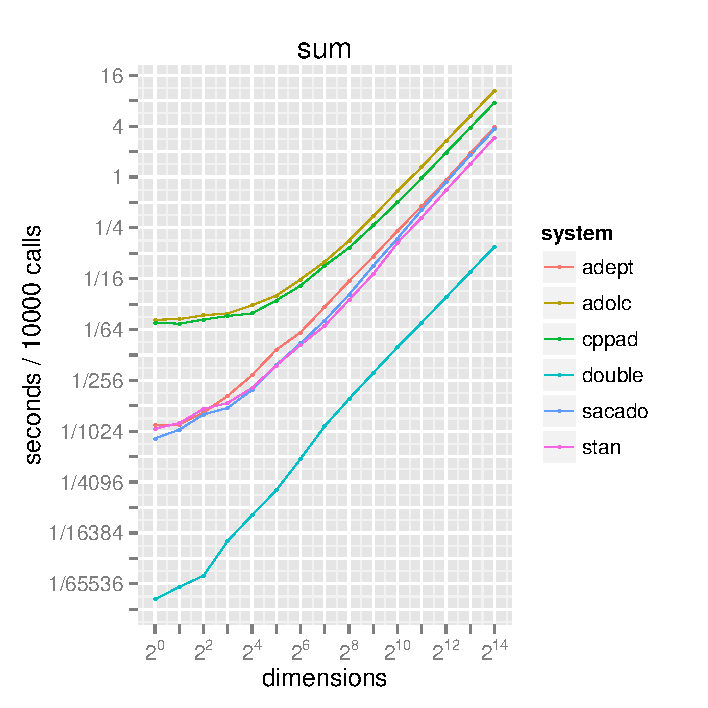
\includegraphics[width=0.48\textwidth]{img/sum_eval.pdf}
\hfill
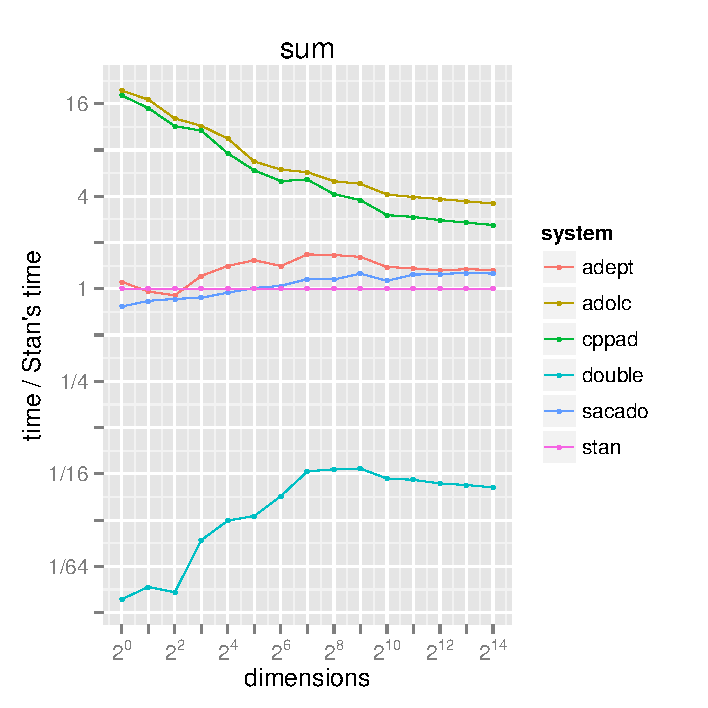
\includegraphics[width=0.48\textwidth]{img/sum_rel_eval.pdf}
\hfill \hfill


\sld{Product \& Log-Sum-Exp}
%
\hfill \hfill
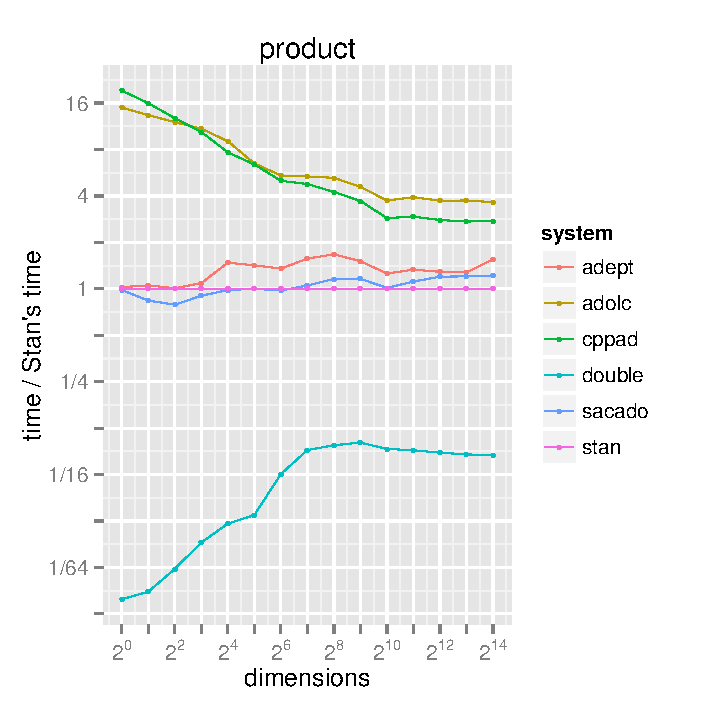
\includegraphics[width=0.45\textwidth]{img/product_rel_eval.pdf}
\hfill
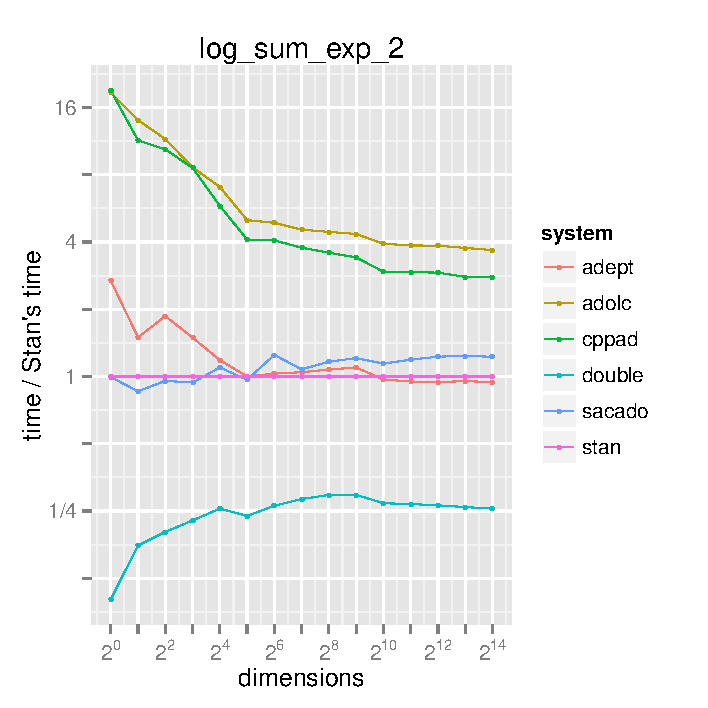
\includegraphics[width=0.45\textwidth]{img/log_sum_exp_2_rel_eval.pdf}
\hfill \hfill


\sld{Stan's Matrix Calculations}
%
\vspace*{-6pt}
\begin{subitemize}
\item Faster in Eigen, but takes more memory
\item Best of both worlds coming soon
\end{subitemize}
\vspace*{-8pt}
\hfill \hfill
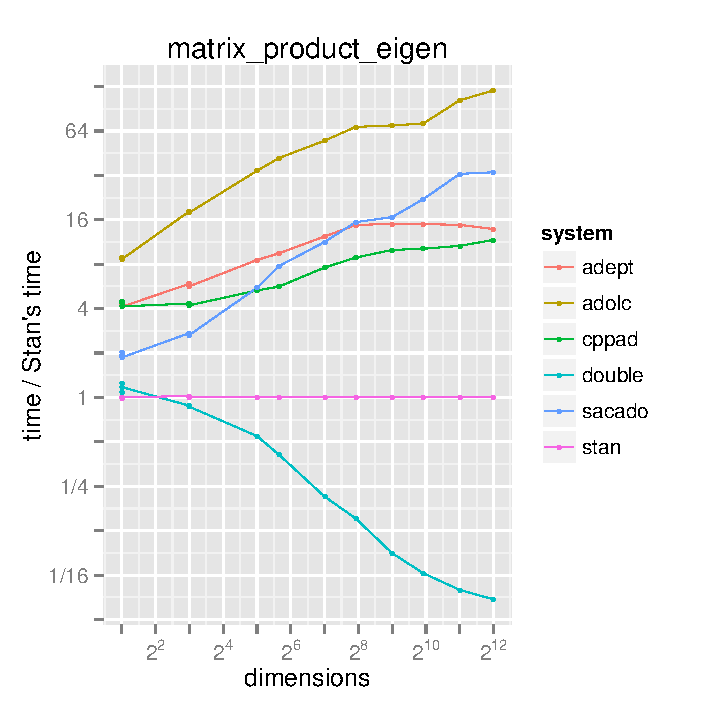
\includegraphics[width=0.48\textwidth]{img/autodiff-eval-matrix-product-eigen.pdf}
\hfill
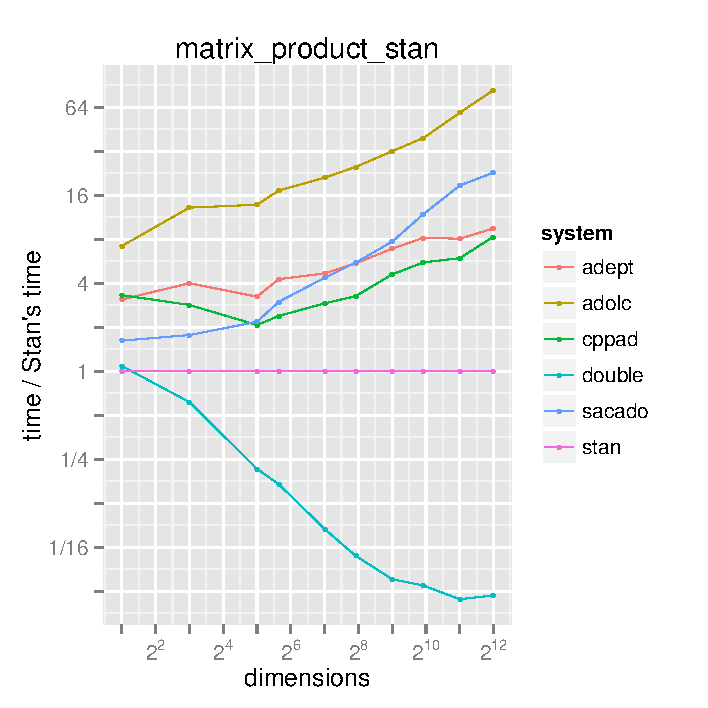
\includegraphics[width=0.48\textwidth]{img/matrix_product_stan_rel_eval.pdf}
\hfill \hfill


\sld{Stan's Density Calculations}
%
\begin{itemize}
\item Vectorization a huge win
\end{itemize}
\vspace*{-8pt}
\hfill \hfill
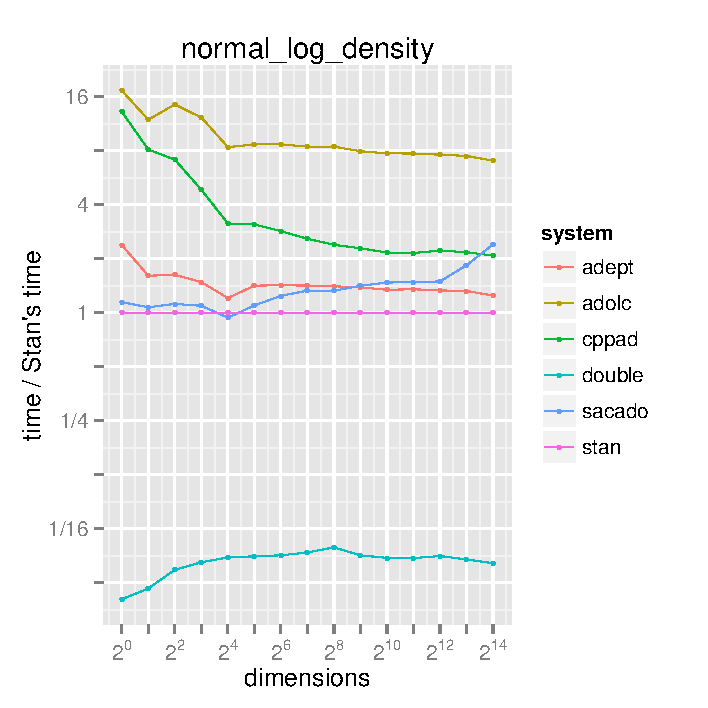
\includegraphics[width=0.48\textwidth]{img/normal_log_density_rel_eval.pdf}
\hfill
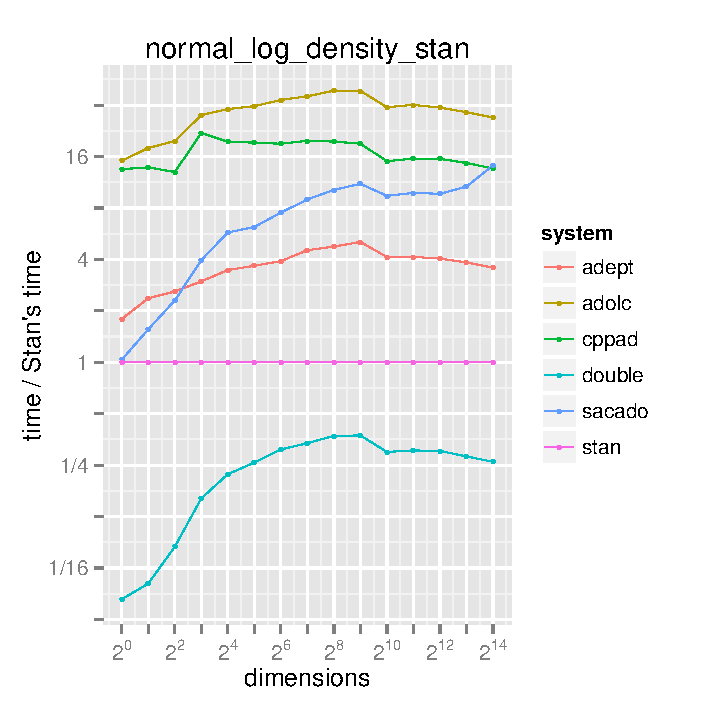
\includegraphics[width=0.48\textwidth]{img/normal_log_density_stan_rel_eval.pdf}
\hfill \hfill


\mypart{}{Autodiff Coding}


\sld{Variable Ptr to Impl}
\begin{stancode}
class var {
public:
  var() : vi_(static_cast<vari*>(0U)) { }
  var(double v) : vi_(new vari(v)) { }

  double val() const { return vi_->val_; }
  double adj() const { return vi_->adj_; }

private:
  vari* vi_;
};
\end{stancode}


\sld{Chainable Base Class}
%
\begin{stancode}
struct chainable {
  chainable() { }
  virtual ~chainable() { }

  virtual void chain() { }
  virtual void init_dependent() { }
  virtual void set_zero_adjoint() { }

  static inline void* operator new(size_t nbytes) {
    return ChainableStack::memalloc_.alloc(nbytes);
  }
};
\end{stancode}


\sld{Variable Implementation}
%
\begin{stancode}
class vari : public chainable {
public:
  const double val_;
  double adj_;

  vari(double v) : val_(v), adj_(0) {
    ChainableStack::var_stack_.push_back(this);
  }

  virtual ~vari() { }

  virtual void init_dependent() { adj_ = 1; }
  virtual void set_zero_adjoint() { adj_ = 0; }
};
\end{stancode}


\sld{Memory Management}
%
\begin{stancode}
struct AutodiffStackStorage {
  static std::vector<chainable*> var_stack_;
  static stack_alloc memalloc_;
};

class stack_alloc {
private:
  std::vector<char*> blocks_;
  std::vector<size_t> sizes_;
  size_t cur_block_;
  char* cur_block_end_;
  char* next_loc_;
  ...
};
\end{stancode}


\sld{Conditional Execution Paths}
%
\begin{stancode}
#ifdef __GNUC__
#define likely(x)      __builtin_expect(!!(x), 1)
#define unlikely(x)    __builtin_expect(!!(x), 0)
#else
#define likely(x)     (x)
#define unlikely(x)   (x)
#endif
\end{stancode}


\sld{Block Allocation}
%
\begin{stancode}
inline void* alloc(size_t len) {
  char* result = next_loc_;
  next_loc_ += len;
  if (unlikely(next_loc_ >= cur_block_end_))
    result = move_to_next_block(len);
  return static_cast<void*>(result);
}
\end{stancode}


\sld{Gradient Calculation}
%
\begin{stancode}
static void grad(chainable* vi) {
  typedef std::vector<chainable*>::reverse_iterator it_t;
  vi->init_dependent();
  it_t begin = ChainableStack::var_stack_.rbegin();
  it_t end = ChainableStack::var_stack_.rend();
  for (it_t it = begin; it < end; ++it)
    (*it)->chain();
}
\end{stancode}


\sld{Unary Function}
%
\begin{stancode}
struct op_v_vari : public vari {
  vari* avi_;

  op_v_vari(double f, vari* avi) : vari(f), avi_(avi) { }
};
\end{stancode}


\sld{Logarithm Implementation}
%
\begin{stancode}
struct log_vari : public op_v_vari {
  log_vari(vari* avi) :
    op_v_vari(std::log(avi->val_), avi) { }

  void chain() {
    avi_->adj_ += adj_ / avi_->val_;
  }
};

inline var log(const var& a) {
  return var(new log_vari(a.vi_));
}
\end{stancode}


\sld{Addition Operator}
%
\begin{stancode}
inline var operator+(const var& a, const var& b) {
  return var(new add_vv_vari(a.vi_, b.vi_));
}

struct add_vari  ...
  void chain() {
    avi_->adj_ += adj_;
    bvi_->adj_ += adj_;
  }

struct product_vari ...
  void chain() {
    avi_->adj_ += adj_ * b_.val();
    bvi_->adj_ += adj_ * a_.val();
  }
\end{stancode}


\sld{Functor for Function}
%
\begin{stancode}
struct normal_ll {
  const Matrix<double, Dynamic, 1> y_;

  normal_ll(const Matrix<double, Dynamic, 1>& y) : y_(y) { }

  template <typename T>
  T operator()(const Matrix<T, Dynamic, 1>& theta) const {
    T mu = theta[0];
    T sigma = theta[1];
    T lp = 0;
    for (int n = 0; n < y_.size(); ++n)
      lp += normal_log(y_[n], mu, sigma);
    return lp;
  }
};
\end{stancode}


\sld{Gradient Functional: Use}
%
\begin{stancode}
Matrix<double, Dynamic, 1> y(3);
y << 1.3, 2.7, -1.9;
normal_ll f(y);

Matrix<double, Dynamic, 1> x(2);
x << 1.3, 2.9;

double fx;
Matrix<double, Dynamic, 1> grad_fx;
stan::math::gradient(f, x, fx, grad_fx);
\end{stancode}


\sld{Gradient Functional}
%
\vspace*{-6pt}
\begin{stancode}
template <typename F>
void gradient(const F& f,  const VectorXd& x,
              double& fx,  VectorXd& grad_fx) {
  try {
    Matrix<var, Dynamic, 1> x_var(x.size());
    for (int i = 0; i < x.size(); ++i) x_var(i) = x(i);
    var fx_var = f(x_var);
    fx = fx_var.val();
    grad(fx_var.vi_);
    grad_fx.resize(x.size());
    for (int i = 0; i < x.size(); ++i)
      grad_fx(i) = x_var(i).adj();
  } catch (const std::exception& /*e*/) {
    recover_memory();   throw;
  }
  recover_memory();
}
\end{stancode}


\mypart{}{Stan for Big(ger) Data}


\sld{Scaling and Evaluation}
%
\begin{center}
\vspace*{-6pt}
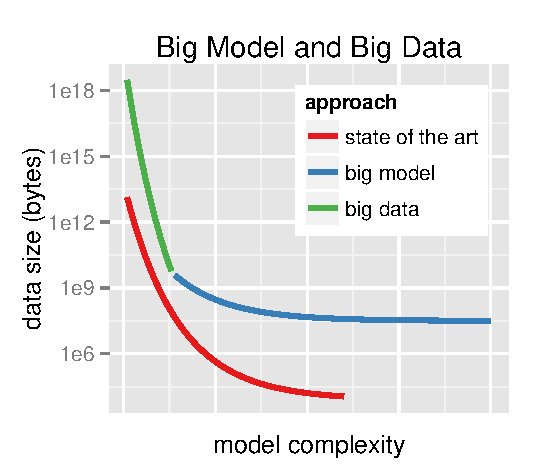
\includegraphics[width=0.6\textwidth]{img/big-model-big-data.pdf}
\vspace*{-6pt}
\end{center}
\begin{itemize}
\item Types of Scaling: data, parameters, \myemph{models}
\end{itemize}


\sld{Riemannian Manifold HMC}
%
\begin{itemize}
\item Best mixing MCMC method (fixed \# of continuous params)
\item Moves on Riemannian manifold rather than Euclidean
\begin{subitemize}
\item adapts to position-dependent curvature
\end{subitemize}
\item \myemph{geoNUTS} generalizes NUTS to RHMC (Betancourt {\slshape arXiv})
\item \myemph{SoftAbs} metric (Betancourt {\slshape arXiv})
\begin{subsubitemize}
\vspace*{-4pt}
\item eigendecompose Hessian and condition
\item computationally feasible alternative to original Fisher info metric
   of Girolami and Calderhead ({\slshape JRSS, Series B})
\item requires third-order derivatives and implicit integrator
\end{subsubitemize}
\vfill
\item merged with develop branch
\end{itemize}


\sld{Adiabatic Sampling}
%
\begin{itemize}
\item Physically motivated alternative to ``simulated''
  \myemph{annealing and tempering} (not really simulated!)
\item Supplies external \myemph{heat bath}
\item Operates through \myemph{contact manifold}
\item System relaxes more naturally between energy levels
\item Betancourt paper on {\slshape arXiv}
  \vfill
\item Prototype complete
\end{itemize}


\sld{Maximum Marginal Mode}
%
\begin{itemize}
\item Fast, approx.\ inference for hierarchical models: $p(\phi, \alpha)$
\item Marginalize out lower-level params: $p(\phi) = \int p(\phi, \alpha) d\alpha$
\item Optimize higher-level parameters $\phi^*$ and fix
\item Optimize lower-level parameters given higher-level: $p(\phi^*, \alpha)$
\item Errors estimated as in MLE
\item aka ``empirical Bayes''
\begin{subitemize}
\item but not fully Bayesian
\item and no more empirical than full Bayes
\end{subitemize}
\item Prototypes in R working
\end{itemize}


\sld{Laplace Approximation}
%
\begin{itemize}
\item Multivariate normal approximation to posterior
\item Compute posterior mode via optimization
\[
\theta^{*} = \argmax_{\theta} \  p(\theta | y)
\]
\item Laplace approximation to the posterior is
\[
p(\theta | y)
\approx
\distro{MultiNormal}(\theta^{*} | -H^{-1})
\]
\item $H$ is the Hessian of the log posterior
\[
H_{i,j}
= \frac{\partial^2}{\partial \theta_i \ \partial \theta_j}
  \log p(\theta | y)
\]
\end{itemize}


\sld{Stan's Laplace Approximation}
%
\begin{itemize}
\item Operates on unconstrained parameters
\item L-BFGS to compute posterior mode $\theta^*$
\item Automatic differentiation to compute $H$
\begin{subitemize}
\item current R: finite differences of gradients
\item soon:  second-order automatic differentiation
\end{subitemize}
\item Draw a sample from approximate posterior
\begin{subitemize}
\item transfrom back to constrained scale
\item allows Monte Carlo computation of expectations
\end{subitemize}
\end{itemize}


\sld{``Black Box'' Variational Inference}
%
\begin{itemize}
%
\item \myemph{Black box} so can fit any Stan model
%
\item Multivariate \myemph{normal approx to unconstrained} posterior
\begin{subitemize}
\item covariance: diagonal mean-field or full rank
\item not Laplace approx --- around posterior mean, not mode
\item transformed back to constrained space (built-in Jacobians)
\end{subitemize}
%
\item Stochastic \myemph{gradient-descent} optimization
\begin{subitemize}
\item ELBO gradient estimated via Monte Carlo + autdiff
\end{subitemize}
%
\item Returns \myemph{approximate posterior} mean / covariance
\item Returns \myemph{sample} transformed to constrained space
\end{itemize}


\sld{VB in a Nutshell}
%
\begin{itemize}
\item $y$ is observed data, $\theta$ parameters
\item Goal is to approximate posterior $p(\theta | y)$
\item with a convenient approximating density $g(\theta | \phi)$
\begin{subitemize}
\item $\phi$ is a vector of parameters of approximating density
\end{subitemize}
\item Given data $y$, VB computes $\phi^*$
minimizing KL-divergence
{\small
\begin{eqnarray*}
\phi^*
& = &
\displaystyle
\argmin_{\phi} \ \mbox{KL}[g(\theta|\phi) \ || \ p(\theta|y)]
\\[4pt]
& = &
\displaystyle
\argmin_{\phi}
\int_{\Theta}
  \log\left(
    \frac{p(\theta \, | \, y)}{g(\theta \, | \, \phi)}
  \right)
  \ g(\theta | \phi) \ \mathrm{d}\theta
\\[4pt]
& = &
\argmin_{\phi} \
\mathbb{E}_{g(\theta|\phi)}\left[\,
  \log p(\theta \, | \, y) - \log g(\theta \, | \, \phi)
\right]
\end{eqnarray*}
}
\end{itemize}


\sld{VB vs.\ Laplace}
%
\vspace*{-6pt}
\begin{center}
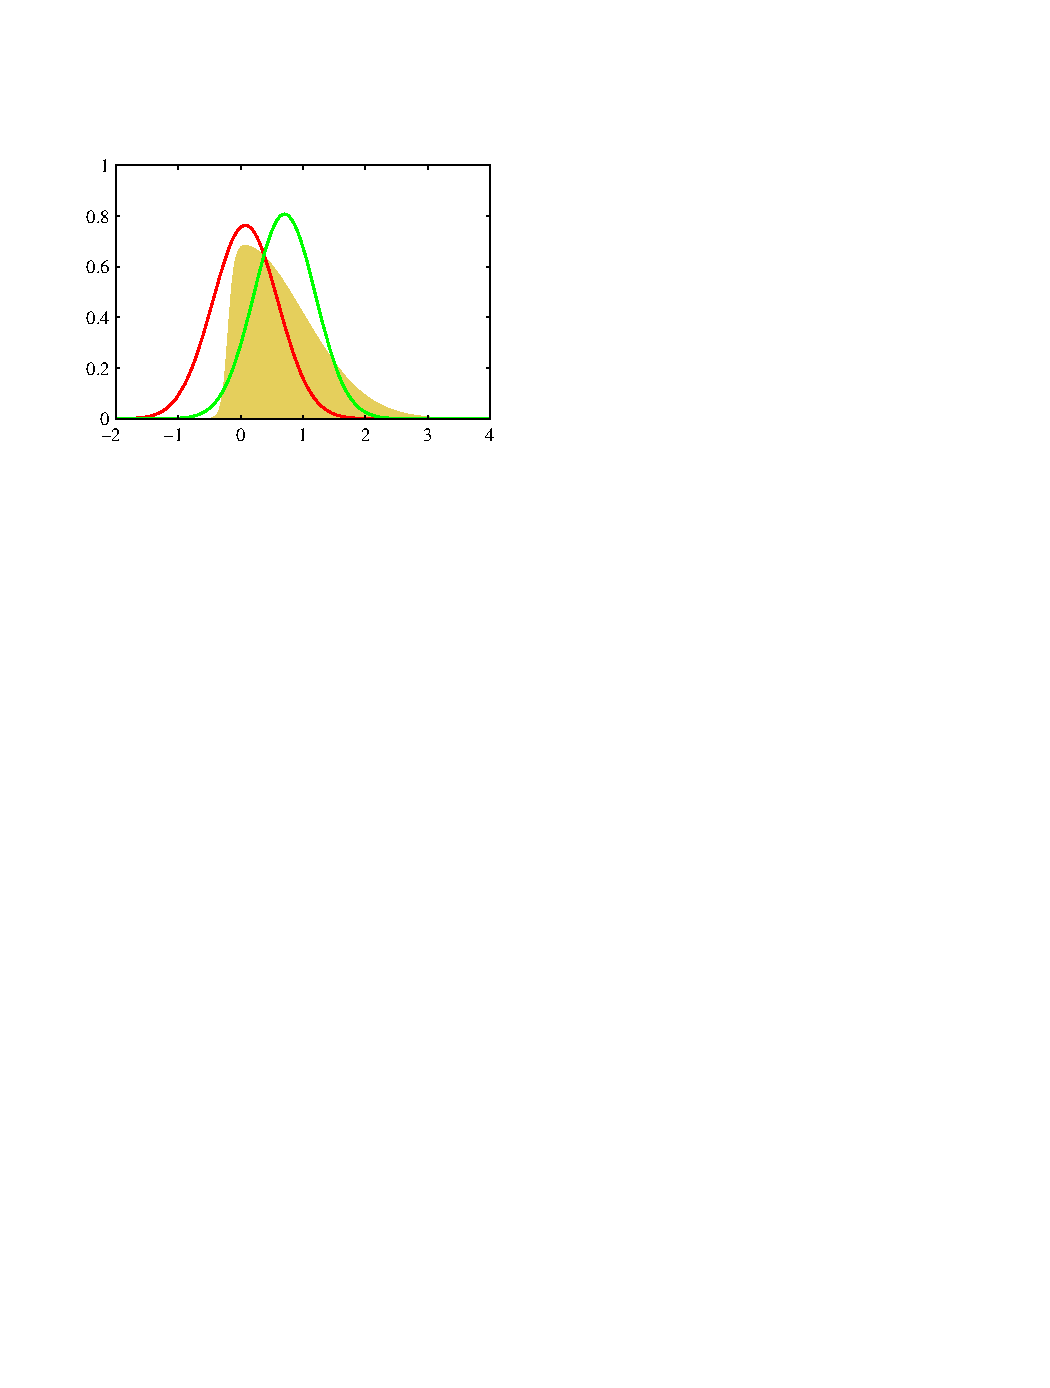
\includegraphics[width=0.45\textwidth]{img/bishop-fig-10-1.pdf}
\end{center}
\vspace*{-10pt}
\begin{itemize}
\item {\slshape solid yellow}: target; \ \ {\slshape red}: Laplace; \ \
  {\slshape green}: VB
\item \myemph{Laplace} located at posterior mode
\item \myemph{VB} located at approximate posterior mean
\end{itemize}
\vfill \hfill
{\footnotesize  --- Bishop (2006) {\slshape Pattern Recognition and Machine Learning}, fig.~10.1}


\sld{KL-Divergence Example}
%
\vspace*{-4pt}
\begin{center}
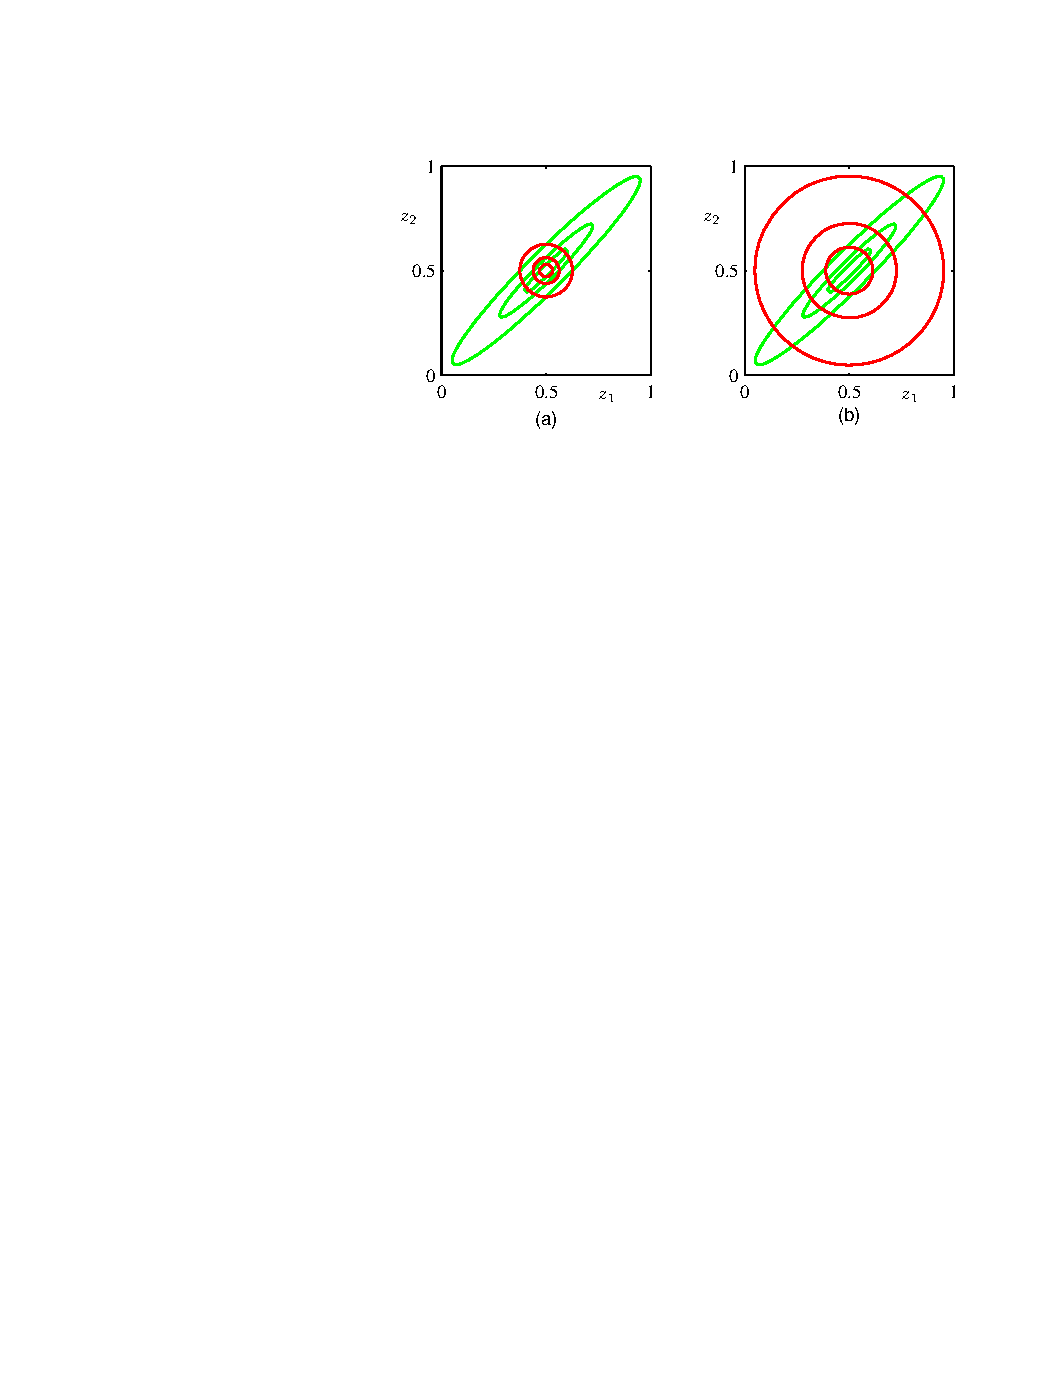
\includegraphics[width=0.6\textwidth]{img/bishop-fig-10-2.pdf}
\end{center}
\vspace*{-10pt}
\begin{subitemize}
\item \myemph{Green}: true distribution $p$; \ \ \myemph{Red}: best
  approximation $g$
\begin{subitemize}
\item[(a)] VB-like: $\mbox{KL}[g \, || \, p]$
\item[(b)] EP-like: $\mbox{KL}[p \, || \, g]$
\end{subitemize}
\item VB systematically \myemph{understimates posterior variance}
\end{subitemize}
\vfill \hfill
{\footnotesize  --- Bishop (2006) {\slshape Pattern Recognition and Machine Learning}, fig.~10.2}


\sld{Stan's ``Black-Box'' VB}
%
\begin{itemize}
\item Typically custom $g()$ per model
\begin{subitemize}
\item based on conjugacy and analytic updates
\end{subitemize}
\item Stan uses ``black-box VB'' with multivariate Gaussian $g$
\[
g(\theta|\phi) = \distro{MultiNormal}(\theta \, | \, \mu, \Sigma)
\]
for the \myemph{unconstrained posterior}
\begin{subitemize}
\item e.g., scales $\sigma$ log-transformed with Jacobian
\end{subitemize}
\item Stan provides two versions
\begin{subitemize}
\item Mean field: $\Sigma$ diagonal
\item General: $\Sigma$ dense
\end{subitemize}
\end{itemize}


\sld{Stan's VB: Computation}
%
\begin{itemize}
\item Use L-BFGS optimization to optimize $\theta$
\item Requires gradient of KL-divergence w.r.t. $\theta$ up to constant
\item Approximate KL-divergence and gradient via Monte Carlo
\begin{subitemize}
\item only need approximate gradient calculation for soundness of L-BFGS
\item KL divergence is an expectation w.r.t. approximation $g(\theta|\phi)$
\item Monte Carlo draws i.i.d.\ from approximating multi-normal
\item derivatives with respect to true model log density via reverse-mode autodiff
\item so only a few Monte Carlo iterations are enough
\end{subitemize}
\end{itemize}


\sld{Stan's VB: Computation (cont.)}
%
\begin{itemize}
\item To support compatible plug-in inference
\begin{subitemize}
\item draw Monte Carlo sample $\theta^{(1)}, \ldots, \theta^{(M)}$ with
\[
\theta^{(m)} \sim  \distro{MultiNormal}(\theta \, | \, \mu^{*}, \Sigma^{*})
\]
\item inverse transfrom from unconstrained to constrained scale
\item report to user in same way as MCMC draws
\vfill
\end{subitemize}
\item Future: reweight $\theta^{(m)}$ via importance sampling
\begin{subitemize}
\item with respect to true posterior
\item to improve expectation calculations
\end{subitemize}
\end{itemize}


\sld{Near Future: Stochastic VB}
%
\begin{itemize}
\item Data-streaming form of VB
\begin{subitemize}
\item Scales to billions of observations
\item {\footnotesize Hoffman et al. (2013) Stochastic variational inference. {\slshape JMLR} 14.}
\end{subitemize}
\item Mashup of stochastic gradient (Robbins and Monro 1951) and VB
\begin{subitemize}
\item subsample data (e.g., stream in minibatches)
\item upweight each minibatch to full data set size
\item use to make unbiased estimate of true gradient
\item take gradient step to minimimize KL-divergence
\end{subitemize}
\vfill
\item Prototype code complete
\end{itemize}


\sld{``Black Box'' EP}
%
\begin{itemize}
\item Fast, approximate inference (like VB)
\begin{subitemize}
\item VB and EP minimize divergence in opposite directions
\item especially useful for Gaussian processes
\end{subitemize}
%
\item Asynchronous, data-parallel \myemph{expectation propagation}
  (EP)
\item Cavity distributions control subsample variance
%
\vfill
%
\item Prototypte stage
\item {\small collaborating with Seth Flaxman, Aki Vehtari, Pasi
    Jyl\"anki, John Cunningham, Nicholas Chopin, Christian Robert}
\end{itemize}

\sld{The Cavity Distribution}
%
\vspace*{-6pt}
\begin{center}

\includegraphics[width=0.25\textwidth]{img/ep-cavity.pdf}
\end{center}
\vspace*{-8pt}
\begin{subitemize}
\item Two parameters, with data split into $y_1, \ldots, y_5$
\item Contours of likelihood $p(y_k | \theta)$ for $k \in 1{:}5$
\item $g_{-k}(\theta)$ is \myemph{cavity distribution} (current
  approx. without $y_k$)
\item Separately computing for $y_k$ reqs each partition to cover its area
\item Combining likelihood with cavity \myemph{focuses on overlap}
\end{subitemize}


\mypart{}{Modeling and Computing\\[8pt]Challenges}


\sld{Discrete Parameters}
%
\begin{itemize}
\item e.g., simple mixture models, survival models, HMMs,
  discrete measurement error models, missing data
\item \myemph{Marginalize out} discrete parameters
\item Efficient sampling due to \myemph{Rao-Blackwellization}
\item Inference straightforward with expectations
  \vspace*{12pt}
\item Too \myemph{difficult} for many of our users
  \\
  {\small (exploring encapsulation options)}
\end{itemize}


\sld{Models with Missing Data}
%
\begin{itemize}
\item In principle, missing data just \myemph{additional parameters}
\item In practice, how to declare?
  \begin{itemize}
  \item \myemph{observed} data as data variables
  \item \myemph{missing} data as parameters
  \item combine into single vector
    \\ {\footnotesize (in transformed parameters or local in model)}
  \end{itemize}
\end{itemize}


\sld{Position-Dependent Curvature}
%
\begin{itemize}
\item Mass matrix does \myemph{global} adaptation for
\begin{subitemize}
\item parameter scale (diagonal) and rotation (dense)
\end{subitemize}
%
\item Dense mass matrices hard to estimate ($\bigoh{N^2}$ estimands)
\item \myemph{Problem}: Position-dependent curvature
\begin{subitemize}
\item Example: banana-shaped densities
\begin{subsubitemize}
\item arise when parameter is product of other parameters
\end{subsubitemize}
\item Example: hierarchical models
\begin{subsubitemize}
\item hierarhcical variance controls lower-level parameters
\end{subsubitemize}
\end{subitemize}
\item Mitigate by reducing stepsize
\begin{subsubitemize}
\item initial (\code{stepsize}) and target acceptance (\code{adapt\_delta})
\end{subsubitemize}
\end{itemize}


\mypart{}{The End}


\mypart{}{Questions?}


\end{document}